\documentclass[twoside]{book}

% Packages required by doxygen
\usepackage{fixltx2e}
\usepackage{calc}
\usepackage{doxygen}
\usepackage[export]{adjustbox} % also loads graphicx
\usepackage{graphicx}
\usepackage[utf8]{inputenc}
\usepackage{makeidx}
\usepackage{multicol}
\usepackage{multirow}
\PassOptionsToPackage{warn}{textcomp}
\usepackage{textcomp}
\usepackage[nointegrals]{wasysym}
\usepackage[table]{xcolor}

% Font selection
\usepackage[T1]{fontenc}
\usepackage[scaled=.90]{helvet}
\usepackage{courier}
\usepackage{amssymb}
\usepackage{sectsty}
\renewcommand{\familydefault}{\sfdefault}
\allsectionsfont{%
  \fontseries{bc}\selectfont%
  \color{darkgray}%
}
\renewcommand{\DoxyLabelFont}{%
  \fontseries{bc}\selectfont%
  \color{darkgray}%
}
\newcommand{\+}{\discretionary{\mbox{\scriptsize$\hookleftarrow$}}{}{}}

% Page & text layout
\usepackage{geometry}
\geometry{%
  letterpaper,%
  top=2.5cm,%
  bottom=2.5cm,%
  left=2.5cm,%
  right=2.5cm%
}
\tolerance=750
\hfuzz=15pt
\hbadness=750
\setlength{\emergencystretch}{15pt}
\setlength{\parindent}{0cm}
\setlength{\parskip}{3ex plus 2ex minus 2ex}
\makeatletter
\renewcommand{\paragraph}{%
  \@startsection{paragraph}{4}{0ex}{-1.0ex}{1.0ex}{%
    \normalfont\normalsize\bfseries\SS@parafont%
  }%
}
\renewcommand{\subparagraph}{%
  \@startsection{subparagraph}{5}{0ex}{-1.0ex}{1.0ex}{%
    \normalfont\normalsize\bfseries\SS@subparafont%
  }%
}
\makeatother

% Headers & footers
\usepackage{fancyhdr}
\pagestyle{fancyplain}
\fancyhead[LE]{\fancyplain{}{\bfseries\thepage}}
\fancyhead[CE]{\fancyplain{}{}}
\fancyhead[RE]{\fancyplain{}{\bfseries\leftmark}}
\fancyhead[LO]{\fancyplain{}{\bfseries\rightmark}}
\fancyhead[CO]{\fancyplain{}{}}
\fancyhead[RO]{\fancyplain{}{\bfseries\thepage}}
\fancyfoot[LE]{\fancyplain{}{}}
\fancyfoot[CE]{\fancyplain{}{}}
\fancyfoot[RE]{\fancyplain{}{\bfseries\scriptsize Generated by Doxygen }}
\fancyfoot[LO]{\fancyplain{}{\bfseries\scriptsize Generated by Doxygen }}
\fancyfoot[CO]{\fancyplain{}{}}
\fancyfoot[RO]{\fancyplain{}{}}
\renewcommand{\footrulewidth}{0.4pt}
\renewcommand{\chaptermark}[1]{%
  \markboth{#1}{}%
}
\renewcommand{\sectionmark}[1]{%
  \markright{\thesection\ #1}%
}

% Indices & bibliography
\usepackage{natbib}
\usepackage[titles]{tocloft}
\setcounter{tocdepth}{3}
\setcounter{secnumdepth}{5}
\makeindex

% Hyperlinks (required, but should be loaded last)
\usepackage{ifpdf}
\ifpdf
  \usepackage[pdftex,pagebackref=true]{hyperref}
\else
  \usepackage[ps2pdf,pagebackref=true]{hyperref}
\fi
\hypersetup{%
  colorlinks=true,%
  linkcolor=blue,%
  citecolor=blue,%
  unicode%
}

% Custom commands
\newcommand{\clearemptydoublepage}{%
  \newpage{\pagestyle{empty}\cleardoublepage}%
}

\usepackage{caption}
\captionsetup{labelsep=space,justification=centering,font={bf},singlelinecheck=off,skip=4pt,position=top}

%===== C O N T E N T S =====

\begin{document}

% Titlepage & ToC
\hypersetup{pageanchor=false,
             bookmarksnumbered=true,
             pdfencoding=unicode
            }
\pagenumbering{roman}
\begin{titlepage}
\vspace*{7cm}
\begin{center}%
{\Large M\+PX Thunder Krakens \\[1ex]\large R2 }\\
\vspace*{1cm}
{\large Generated by Doxygen 1.8.11}\\
\end{center}
\end{titlepage}
\clearemptydoublepage
\tableofcontents
\clearemptydoublepage
\pagenumbering{arabic}
\hypersetup{pageanchor=true}

%--- Begin generated contents ---
\chapter{Main Page}
\label{index}\hypertarget{index}{}Welcome to the Programmer’s manual for the Thunder Kracken’s M\+PX Operating system. This document catalogues all of the information one may need to know regarding the use and modification of this Operating system and its contents. Included is a complete A\+PI of every method created for the operating system which includes all inputs and outputs as well as a brief summary of the purpose of each method. This will give you a more in depth look at all of the ordinary user commands as well as the internal commands used to perform functions that normal users cannot access. Most likely these commands will be the most important for making new programs on the operating system. This document also lists the documentation for the files files in the operating system. This includes all of the variables and methods used in each file. These will help direct you as to where certain functions are defined. For general usage tips, please refer to the user manual. We hope you find working with the Thunder Kracken’s M\+PX Operating System as enjoyable as we do and we thank you for using our product. 
\chapter{Data Structure Index}
\section{Class List}
Here are the classes, structs, unions and interfaces with brief descriptions\+:\begin{DoxyCompactList}
\item\contentsline{section}{\hyperlink{structfunction__name}{function\+\_\+name} }{\pageref{structfunction__name}}{}
\end{DoxyCompactList}

\chapter{File Index}
\section{File List}
Here is a list of all files with brief descriptions\+:\begin{DoxyCompactList}
\item\contentsline{section}{include/\hyperlink{string_8h}{string.\+h} \\*Many usefull functions that used for handling string }{\pageref{string_8h}}{}
\item\contentsline{section}{include/core/\hyperlink{serial_8h}{serial.\+h} \\*Serial -\/ Header }{\pageref{serial_8h}}{}
\item\contentsline{section}{lib/\hyperlink{string_8c}{string.\+c} \\*Many usefull functions that used for handling string }{\pageref{string_8c}}{}
\item\contentsline{section}{modules/\hyperlink{errno_8h}{errno.\+h} \\*This file contains the type of errors. The error can be from invalid paramter passed to a function, or invalid input format }{\pageref{errno_8h}}{}
\item\contentsline{section}{modules/r1/\hyperlink{r1_8c}{r1.\+c} \\*The commandhander and functions associations for Module R1 }{\pageref{r1_8c}}{}
\item\contentsline{section}{modules/r1/\hyperlink{r1_8h}{r1.\+h} \\*The commandhander and functions associations for Module R1 }{\pageref{r1_8h}}{}
\item\contentsline{section}{modules/r1/\hyperlink{sys__clock_8c}{sys\+\_\+clock.\+c} \\*The main file that manipulates and controls the system\textquotesingle{}s clock }{\pageref{sys__clock_8c}}{}
\item\contentsline{section}{modules/r1/\hyperlink{sys__clock_8h}{sys\+\_\+clock.\+h} \\*The main file that manipulates and controls the system\textquotesingle{}s clock }{\pageref{sys__clock_8h}}{}
\item\contentsline{section}{modules/r2/\hyperlink{pcb_8c}{pcb.\+c} \\*The Process Control Block }{\pageref{pcb_8c}}{}
\item\contentsline{section}{modules/r2/\hyperlink{pcb_8h}{pcb.\+h} \\*The Process Control Block }{\pageref{pcb_8h}}{}
\item\contentsline{section}{modules/r2/\hyperlink{pcb__comm_8c}{pcb\+\_\+comm.\+c} \\*The main functions that manipulate the P\+CB }{\pageref{pcb__comm_8c}}{}
\item\contentsline{section}{modules/r2/\hyperlink{pcb__comm_8h}{pcb\+\_\+comm.\+h} \\*The main functions that manipulate the P\+CB }{\pageref{pcb__comm_8h}}{}
\end{DoxyCompactList}

\chapter{Data Structure Documentation}
\hypertarget{structfunction__name}{}\section{function\+\_\+name Struct Reference}
\label{structfunction__name}\index{function\+\_\+name@{function\+\_\+name}}
\subsection*{Public Attributes}
\begin{DoxyCompactItemize}
\item 
char $\ast$ {\bfseries name\+Str}\hypertarget{structfunction__name_a7a94f7f31542a15b63160b6b213e0bcb}{}\label{structfunction__name_a7a94f7f31542a15b63160b6b213e0bcb}

\item 
int($\ast$ {\bfseries function} )(int argc, char $\ast$$\ast$argv)\hypertarget{structfunction__name_ad80214b3eea6c438c13ff5461c5350ab}{}\label{structfunction__name_ad80214b3eea6c438c13ff5461c5350ab}

\item 
char $\ast$ {\bfseries usage}\hypertarget{structfunction__name_a30f593e52febda0cc9d9703b9015fb0f}{}\label{structfunction__name_a30f593e52febda0cc9d9703b9015fb0f}

\item 
char $\ast$ {\bfseries help}\hypertarget{structfunction__name_ac0f73e570d7d03a9f378a70e6d4d5632}{}\label{structfunction__name_ac0f73e570d7d03a9f378a70e6d4d5632}

\end{DoxyCompactItemize}


The documentation for this struct was generated from the following file\+:\begin{DoxyCompactItemize}
\item 
modules/r1/\hyperlink{r1_8h}{r1.\+h}\end{DoxyCompactItemize}

\hypertarget{structpcb__queue}{}\section{pcb\+\_\+queue Struct Reference}
\label{structpcb__queue}\index{pcb\+\_\+queue@{pcb\+\_\+queue}}


Queue structure that will store P\+C\+Bs.  




{\ttfamily \#include $<$pcb.\+h$>$}



Collaboration diagram for pcb\+\_\+queue\+:\nopagebreak
\begin{figure}[H]
\begin{center}
\leavevmode
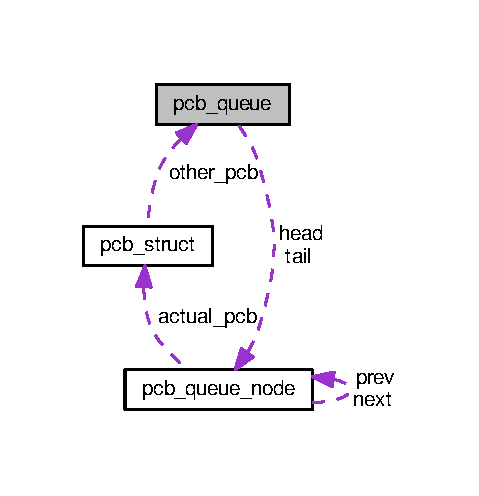
\includegraphics[width=230pt]{structpcb__queue__coll__graph}
\end{center}
\end{figure}
\subsection*{Data Fields}
\begin{DoxyCompactItemize}
\item 
int \hyperlink{structpcb__queue_a04e6c9d91e324b1f6cbc8bfd771bafb1}{count}
\begin{DoxyCompactList}\small\item\em The length of the queue. \end{DoxyCompactList}\item 
struct \hyperlink{structpcb__queue__node}{pcb\+\_\+queue\+\_\+node} $\ast$ \hyperlink{structpcb__queue_a183818f26c833aa30aefac583db68388}{head}
\begin{DoxyCompactList}\small\item\em Pointer to the start/head of the queue. \end{DoxyCompactList}\item 
struct \hyperlink{structpcb__queue__node}{pcb\+\_\+queue\+\_\+node} $\ast$ \hyperlink{structpcb__queue_a54ed164636944248130e7032b7786cb3}{tail}
\begin{DoxyCompactList}\small\item\em Pointer to the end/tail of the queue. \end{DoxyCompactList}\end{DoxyCompactItemize}


\subsection{Detailed Description}
Queue structure that will store P\+C\+Bs. 

\subsection{Field Documentation}
\index{pcb\+\_\+queue@{pcb\+\_\+queue}!count@{count}}
\index{count@{count}!pcb\+\_\+queue@{pcb\+\_\+queue}}
\subsubsection[{\texorpdfstring{count}{count}}]{\setlength{\rightskip}{0pt plus 5cm}int pcb\+\_\+queue\+::count}\hypertarget{structpcb__queue_a04e6c9d91e324b1f6cbc8bfd771bafb1}{}\label{structpcb__queue_a04e6c9d91e324b1f6cbc8bfd771bafb1}


The length of the queue. 

\index{pcb\+\_\+queue@{pcb\+\_\+queue}!head@{head}}
\index{head@{head}!pcb\+\_\+queue@{pcb\+\_\+queue}}
\subsubsection[{\texorpdfstring{head}{head}}]{\setlength{\rightskip}{0pt plus 5cm}struct {\bf pcb\+\_\+queue\+\_\+node}$\ast$ pcb\+\_\+queue\+::head}\hypertarget{structpcb__queue_a183818f26c833aa30aefac583db68388}{}\label{structpcb__queue_a183818f26c833aa30aefac583db68388}


Pointer to the start/head of the queue. 

\index{pcb\+\_\+queue@{pcb\+\_\+queue}!tail@{tail}}
\index{tail@{tail}!pcb\+\_\+queue@{pcb\+\_\+queue}}
\subsubsection[{\texorpdfstring{tail}{tail}}]{\setlength{\rightskip}{0pt plus 5cm}struct {\bf pcb\+\_\+queue\+\_\+node}$\ast$ pcb\+\_\+queue\+::tail}\hypertarget{structpcb__queue_a54ed164636944248130e7032b7786cb3}{}\label{structpcb__queue_a54ed164636944248130e7032b7786cb3}


Pointer to the end/tail of the queue. 



The documentation for this struct was generated from the following file\+:\begin{DoxyCompactItemize}
\item 
modules/r2/\hyperlink{pcb_8h}{pcb.\+h}\end{DoxyCompactItemize}

\hypertarget{structpcb__queue__node}{}\section{pcb\+\_\+queue\+\_\+node Struct Reference}
\label{structpcb__queue__node}\index{pcb\+\_\+queue\+\_\+node@{pcb\+\_\+queue\+\_\+node}}


The P\+CB queue node will represent the P\+CB within \hyperlink{structpcb__queue}{pcb\+\_\+queue} and point to previous/next P\+CB nodes.  




{\ttfamily \#include $<$pcb.\+h$>$}



Collaboration diagram for pcb\+\_\+queue\+\_\+node\+:\nopagebreak
\begin{figure}[H]
\begin{center}
\leavevmode
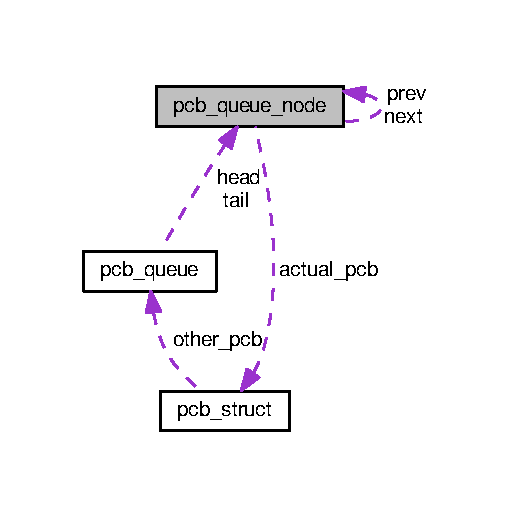
\includegraphics[width=245pt]{structpcb__queue__node__coll__graph}
\end{center}
\end{figure}
\subsection*{Data Fields}
\begin{DoxyCompactItemize}
\item 
struct \hyperlink{structpcb__queue__node}{pcb\+\_\+queue\+\_\+node} $\ast$ \hyperlink{structpcb__queue__node_aff49de430038d879a5a58105aa1544d5}{prev}
\begin{DoxyCompactList}\small\item\em Pointer to the previous P\+CB in the queue. \end{DoxyCompactList}\item 
struct \hyperlink{structpcb__struct}{pcb\+\_\+struct} \hyperlink{structpcb__queue__node_aec85184e42b89d83290f46d292a9c2df}{actual\+\_\+pcb}
\begin{DoxyCompactList}\small\item\em Pointer to the P\+CB process. \end{DoxyCompactList}\item 
struct \hyperlink{structpcb__queue__node}{pcb\+\_\+queue\+\_\+node} $\ast$ \hyperlink{structpcb__queue__node_a6634871cb99f4f53fed51e9b51f6852c}{next}
\begin{DoxyCompactList}\small\item\em Pointer to the next P\+CB in the queue. \end{DoxyCompactList}\end{DoxyCompactItemize}


\subsection{Detailed Description}
The P\+CB queue node will represent the P\+CB within \hyperlink{structpcb__queue}{pcb\+\_\+queue} and point to previous/next P\+CB nodes. 

This structure is a doubly linked list. 

\subsection{Field Documentation}
\index{pcb\+\_\+queue\+\_\+node@{pcb\+\_\+queue\+\_\+node}!actual\+\_\+pcb@{actual\+\_\+pcb}}
\index{actual\+\_\+pcb@{actual\+\_\+pcb}!pcb\+\_\+queue\+\_\+node@{pcb\+\_\+queue\+\_\+node}}
\subsubsection[{\texorpdfstring{actual\+\_\+pcb}{actual_pcb}}]{\setlength{\rightskip}{0pt plus 5cm}struct {\bf pcb\+\_\+struct} pcb\+\_\+queue\+\_\+node\+::actual\+\_\+pcb}\hypertarget{structpcb__queue__node_aec85184e42b89d83290f46d292a9c2df}{}\label{structpcb__queue__node_aec85184e42b89d83290f46d292a9c2df}


Pointer to the P\+CB process. 

\index{pcb\+\_\+queue\+\_\+node@{pcb\+\_\+queue\+\_\+node}!next@{next}}
\index{next@{next}!pcb\+\_\+queue\+\_\+node@{pcb\+\_\+queue\+\_\+node}}
\subsubsection[{\texorpdfstring{next}{next}}]{\setlength{\rightskip}{0pt plus 5cm}struct {\bf pcb\+\_\+queue\+\_\+node}$\ast$ pcb\+\_\+queue\+\_\+node\+::next}\hypertarget{structpcb__queue__node_a6634871cb99f4f53fed51e9b51f6852c}{}\label{structpcb__queue__node_a6634871cb99f4f53fed51e9b51f6852c}


Pointer to the next P\+CB in the queue. 

\index{pcb\+\_\+queue\+\_\+node@{pcb\+\_\+queue\+\_\+node}!prev@{prev}}
\index{prev@{prev}!pcb\+\_\+queue\+\_\+node@{pcb\+\_\+queue\+\_\+node}}
\subsubsection[{\texorpdfstring{prev}{prev}}]{\setlength{\rightskip}{0pt plus 5cm}struct {\bf pcb\+\_\+queue\+\_\+node}$\ast$ pcb\+\_\+queue\+\_\+node\+::prev}\hypertarget{structpcb__queue__node_aff49de430038d879a5a58105aa1544d5}{}\label{structpcb__queue__node_aff49de430038d879a5a58105aa1544d5}


Pointer to the previous P\+CB in the queue. 



The documentation for this struct was generated from the following file\+:\begin{DoxyCompactItemize}
\item 
modules/r2/\hyperlink{pcb_8h}{pcb.\+h}\end{DoxyCompactItemize}

\hypertarget{structpcb__struct}{}\section{pcb\+\_\+struct Struct Reference}
\label{structpcb__struct}\index{pcb\+\_\+struct@{pcb\+\_\+struct}}


Struct that will describe P\+CB Processes.  




{\ttfamily \#include $<$pcb.\+h$>$}



Collaboration diagram for pcb\+\_\+struct\+:\nopagebreak
\begin{figure}[H]
\begin{center}
\leavevmode
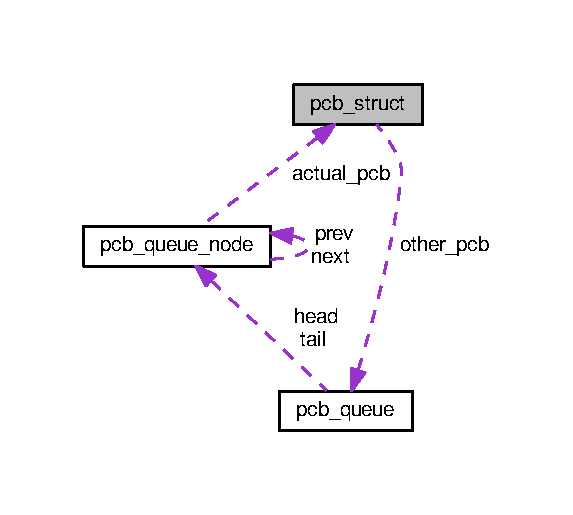
\includegraphics[width=275pt]{structpcb__struct__coll__graph}
\end{center}
\end{figure}
\subsection*{Data Fields}
\begin{DoxyCompactItemize}
\item 
char \hyperlink{structpcb__struct_a2bd5a2bbfc9b13812cec1c884077930e}{name} \mbox{[}10\mbox{]}
\begin{DoxyCompactList}\small\item\em P\+CB\textquotesingle{}s name. \end{DoxyCompactList}\item 
enum \hyperlink{pcb_8h_aefe309d62b55b4d0be96f1a97fcbbadd}{process\+\_\+class} \hyperlink{structpcb__struct_a3957f5586930529631c9a428a30b7325}{class}
\begin{DoxyCompactList}\small\item\em P\+CB\textquotesingle{}s class is an application or system process. \end{DoxyCompactList}\item 
unsigned char \hyperlink{structpcb__struct_aff2a92397b2ef3d680c09934ecd5f032}{priority}
\begin{DoxyCompactList}\small\item\em P\+CB\textquotesingle{}s priority an integer between 0 and 9. \end{DoxyCompactList}\item 
enum \hyperlink{pcb_8h_a4e1a76273cf189daed25256e3ba34aef}{process\+\_\+state} \hyperlink{structpcb__struct_a374d522318eb94188698cbb5bd85009d}{running\+\_\+state}
\begin{DoxyCompactList}\small\item\em P\+CB\textquotesingle{}s states are ready, running, or blocked. \end{DoxyCompactList}\item 
enum \hyperlink{pcb_8h_ac80b09976226d1f179d0911462a93034}{process\+\_\+suspended} \hyperlink{structpcb__struct_aefb20b3b3c88e40e18ed2b505262d788}{is\+\_\+suspended}
\begin{DoxyCompactList}\small\item\em P\+CB process is either suspended or not suspended. \end{DoxyCompactList}\item 
unsigned char $\ast$ \hyperlink{structpcb__struct_a277e7babba5b14dc71ffc08bf69f54c3}{stack\+\_\+top}
\begin{DoxyCompactList}\small\item\em Pointer to top of the stack. \end{DoxyCompactList}\item 
unsigned char $\ast$ \hyperlink{structpcb__struct_a8365cb3b483002fecc259df14301f30f}{stack\+\_\+base}
\begin{DoxyCompactList}\small\item\em Pointer to base of the stack. \end{DoxyCompactList}\item 
struct \hyperlink{structpcb__queue}{pcb\+\_\+queue} $\ast$ \hyperlink{structpcb__struct_aba9f99ef03e34c9f9ef79053a255ba27}{other\+\_\+pcb}
\begin{DoxyCompactList}\small\item\em Pointer to other P\+C\+Bs. \end{DoxyCompactList}\end{DoxyCompactItemize}


\subsection{Detailed Description}
Struct that will describe P\+CB Processes. 

\subsection{Field Documentation}
\index{pcb\+\_\+struct@{pcb\+\_\+struct}!class@{class}}
\index{class@{class}!pcb\+\_\+struct@{pcb\+\_\+struct}}
\subsubsection[{\texorpdfstring{class}{class}}]{\setlength{\rightskip}{0pt plus 5cm}enum {\bf process\+\_\+class} pcb\+\_\+struct\+::class}\hypertarget{structpcb__struct_a3957f5586930529631c9a428a30b7325}{}\label{structpcb__struct_a3957f5586930529631c9a428a30b7325}


P\+CB\textquotesingle{}s class is an application or system process. 

\index{pcb\+\_\+struct@{pcb\+\_\+struct}!is\+\_\+suspended@{is\+\_\+suspended}}
\index{is\+\_\+suspended@{is\+\_\+suspended}!pcb\+\_\+struct@{pcb\+\_\+struct}}
\subsubsection[{\texorpdfstring{is\+\_\+suspended}{is_suspended}}]{\setlength{\rightskip}{0pt plus 5cm}enum {\bf process\+\_\+suspended} pcb\+\_\+struct\+::is\+\_\+suspended}\hypertarget{structpcb__struct_aefb20b3b3c88e40e18ed2b505262d788}{}\label{structpcb__struct_aefb20b3b3c88e40e18ed2b505262d788}


P\+CB process is either suspended or not suspended. 

\index{pcb\+\_\+struct@{pcb\+\_\+struct}!name@{name}}
\index{name@{name}!pcb\+\_\+struct@{pcb\+\_\+struct}}
\subsubsection[{\texorpdfstring{name}{name}}]{\setlength{\rightskip}{0pt plus 5cm}char pcb\+\_\+struct\+::name\mbox{[}10\mbox{]}}\hypertarget{structpcb__struct_a2bd5a2bbfc9b13812cec1c884077930e}{}\label{structpcb__struct_a2bd5a2bbfc9b13812cec1c884077930e}


P\+CB\textquotesingle{}s name. 

\index{pcb\+\_\+struct@{pcb\+\_\+struct}!other\+\_\+pcb@{other\+\_\+pcb}}
\index{other\+\_\+pcb@{other\+\_\+pcb}!pcb\+\_\+struct@{pcb\+\_\+struct}}
\subsubsection[{\texorpdfstring{other\+\_\+pcb}{other_pcb}}]{\setlength{\rightskip}{0pt plus 5cm}struct {\bf pcb\+\_\+queue}$\ast$ pcb\+\_\+struct\+::other\+\_\+pcb}\hypertarget{structpcb__struct_aba9f99ef03e34c9f9ef79053a255ba27}{}\label{structpcb__struct_aba9f99ef03e34c9f9ef79053a255ba27}


Pointer to other P\+C\+Bs. 

\index{pcb\+\_\+struct@{pcb\+\_\+struct}!priority@{priority}}
\index{priority@{priority}!pcb\+\_\+struct@{pcb\+\_\+struct}}
\subsubsection[{\texorpdfstring{priority}{priority}}]{\setlength{\rightskip}{0pt plus 5cm}unsigned char pcb\+\_\+struct\+::priority}\hypertarget{structpcb__struct_aff2a92397b2ef3d680c09934ecd5f032}{}\label{structpcb__struct_aff2a92397b2ef3d680c09934ecd5f032}


P\+CB\textquotesingle{}s priority an integer between 0 and 9. 

Processes with higher priority values execute before lower priority processes. \index{pcb\+\_\+struct@{pcb\+\_\+struct}!running\+\_\+state@{running\+\_\+state}}
\index{running\+\_\+state@{running\+\_\+state}!pcb\+\_\+struct@{pcb\+\_\+struct}}
\subsubsection[{\texorpdfstring{running\+\_\+state}{running_state}}]{\setlength{\rightskip}{0pt plus 5cm}enum {\bf process\+\_\+state} pcb\+\_\+struct\+::running\+\_\+state}\hypertarget{structpcb__struct_a374d522318eb94188698cbb5bd85009d}{}\label{structpcb__struct_a374d522318eb94188698cbb5bd85009d}


P\+CB\textquotesingle{}s states are ready, running, or blocked. 

\index{pcb\+\_\+struct@{pcb\+\_\+struct}!stack\+\_\+base@{stack\+\_\+base}}
\index{stack\+\_\+base@{stack\+\_\+base}!pcb\+\_\+struct@{pcb\+\_\+struct}}
\subsubsection[{\texorpdfstring{stack\+\_\+base}{stack_base}}]{\setlength{\rightskip}{0pt plus 5cm}unsigned char$\ast$ pcb\+\_\+struct\+::stack\+\_\+base}\hypertarget{structpcb__struct_a8365cb3b483002fecc259df14301f30f}{}\label{structpcb__struct_a8365cb3b483002fecc259df14301f30f}


Pointer to base of the stack. 

\index{pcb\+\_\+struct@{pcb\+\_\+struct}!stack\+\_\+top@{stack\+\_\+top}}
\index{stack\+\_\+top@{stack\+\_\+top}!pcb\+\_\+struct@{pcb\+\_\+struct}}
\subsubsection[{\texorpdfstring{stack\+\_\+top}{stack_top}}]{\setlength{\rightskip}{0pt plus 5cm}unsigned char$\ast$ pcb\+\_\+struct\+::stack\+\_\+top}\hypertarget{structpcb__struct_a277e7babba5b14dc71ffc08bf69f54c3}{}\label{structpcb__struct_a277e7babba5b14dc71ffc08bf69f54c3}


Pointer to top of the stack. 



The documentation for this struct was generated from the following file\+:\begin{DoxyCompactItemize}
\item 
modules/r2/\hyperlink{pcb_8h}{pcb.\+h}\end{DoxyCompactItemize}

\chapter{File Documentation}
\hypertarget{mainpage_8dox}{}\section{documentation/mainpage.dox File Reference}
\label{mainpage_8dox}\index{documentation/mainpage.\+dox@{documentation/mainpage.\+dox}}

\hypertarget{serial_8h}{}\section{include/core/serial.h File Reference}
\label{serial_8h}\index{include/core/serial.\+h@{include/core/serial.\+h}}


Serial -\/ Header.  


\subsection*{Macros}
\begin{DoxyCompactItemize}
\item 
\#define {\bfseries C\+O\+M1}~0x3f8\hypertarget{serial_8h_a00dbb3ab1c59e14699be9393693e2248}{}\label{serial_8h_a00dbb3ab1c59e14699be9393693e2248}

\item 
\#define {\bfseries C\+O\+M2}~0x2f8\hypertarget{serial_8h_a435e02f194c24c9b0e00d7cd27a1704e}{}\label{serial_8h_a435e02f194c24c9b0e00d7cd27a1704e}

\item 
\#define {\bfseries C\+O\+M3}~0x3e8\hypertarget{serial_8h_abbed02672431595364c5dd35809303a6}{}\label{serial_8h_abbed02672431595364c5dd35809303a6}

\item 
\#define {\bfseries C\+O\+M4}~0x2e8\hypertarget{serial_8h_a595cabb01568ba641574d24546d99c6b}{}\label{serial_8h_a595cabb01568ba641574d24546d99c6b}

\item 
\#define {\bfseries Without\+Echo}~0\hypertarget{serial_8h_a99c15aced355f0ca133b05cf46a7ff28}{}\label{serial_8h_a99c15aced355f0ca133b05cf46a7ff28}

\item 
\#define {\bfseries With\+Echo}~1\hypertarget{serial_8h_afddb5e7f7cc4e3632a18609dabf32628}{}\label{serial_8h_afddb5e7f7cc4e3632a18609dabf32628}

\end{DoxyCompactItemize}
\subsection*{Functions}
\begin{DoxyCompactItemize}
\item 
int {\bfseries init\+\_\+serial} (int device)\hypertarget{serial_8h_a7078c07ff8b2c48780558549a8f7cf90}{}\label{serial_8h_a7078c07ff8b2c48780558549a8f7cf90}

\item 
int {\bfseries serial\+\_\+println} (const char $\ast$msg)\hypertarget{serial_8h_a3514f7abff236a4e00a6c46021ce5e22}{}\label{serial_8h_a3514f7abff236a4e00a6c46021ce5e22}

\item 
int {\bfseries serial\+\_\+print} (const char $\ast$msg)\hypertarget{serial_8h_a995827efcd4dcfb780c9fbb9645410a4}{}\label{serial_8h_a995827efcd4dcfb780c9fbb9645410a4}

\item 
int {\bfseries set\+\_\+serial\+\_\+out} (int device)\hypertarget{serial_8h_ae97b87ee1f57c687e7fca6f9958e03ef}{}\label{serial_8h_ae97b87ee1f57c687e7fca6f9958e03ef}

\item 
int {\bfseries set\+\_\+serial\+\_\+in} (int device)\hypertarget{serial_8h_a3f4008da5feabfb7e086f6673a81104b}{}\label{serial_8h_a3f4008da5feabfb7e086f6673a81104b}

\item 
void \hyperlink{serial_8h_aca81fe61abc40b171257825521578e6c}{get\+\_\+input\+\_\+line} (char $\ast$buffer, const int buffer\+\_\+size, const int b\+With\+Echo)
\begin{DoxyCompactList}\small\item\em get\+\_\+input\+\_\+line. \end{DoxyCompactList}\end{DoxyCompactItemize}


\subsection{Detailed Description}
Serial -\/ Header. 

\begin{DoxyAuthor}{Author}
Thunder Krakens 
\end{DoxyAuthor}
\begin{DoxyDate}{Date}
February 2nd, 2016 
\end{DoxyDate}
\begin{DoxyVersion}{Version}
R1 
\end{DoxyVersion}


\subsection{Function Documentation}
\index{serial.\+h@{serial.\+h}!get\+\_\+input\+\_\+line@{get\+\_\+input\+\_\+line}}
\index{get\+\_\+input\+\_\+line@{get\+\_\+input\+\_\+line}!serial.\+h@{serial.\+h}}
\subsubsection[{\texorpdfstring{get\+\_\+input\+\_\+line(char $\ast$buffer, const int buffer\+\_\+size, const int b\+With\+Echo)}{get_input_line(char *buffer, const int buffer_size, const int bWithEcho)}}]{\setlength{\rightskip}{0pt plus 5cm}void get\+\_\+input\+\_\+line (
\begin{DoxyParamCaption}
\item[{char $\ast$}]{buffer, }
\item[{const int}]{buffer\+\_\+size, }
\item[{const int}]{b\+With\+Echo}
\end{DoxyParamCaption}
)}\hypertarget{serial_8h_aca81fe61abc40b171257825521578e6c}{}\label{serial_8h_aca81fe61abc40b171257825521578e6c}


get\+\_\+input\+\_\+line. 

Description\+: Get user\textquotesingle{}s input from keyborad. 
\begin{DoxyParams}{Parameters}
{\em buffer} & -\/ The pointer to the buffer where store the user\textquotesingle{}s input. \\
\hline
{\em buffer\+\_\+size} & -\/ The size of that buffer. \\
\hline
{\em b\+With\+Echo} & -\/ With echo or not \\
\hline
\end{DoxyParams}
\begin{DoxyReturn}{Returns}
V\+O\+ID 
\end{DoxyReturn}

\hypertarget{string_8h}{}\section{include/string.h File Reference}
\label{string_8h}\index{include/string.\+h@{include/string.\+h}}


Many usefull functions that used for handling string.  


{\ttfamily \#include $<$system.\+h$>$}\\*
Include dependency graph for string.\+h\+:
\nopagebreak
\begin{figure}[H]
\begin{center}
\leavevmode
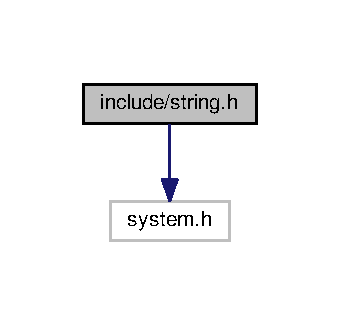
\includegraphics[width=163pt]{string_8h__incl}
\end{center}
\end{figure}
This graph shows which files directly or indirectly include this file\+:
\nopagebreak
\begin{figure}[H]
\begin{center}
\leavevmode
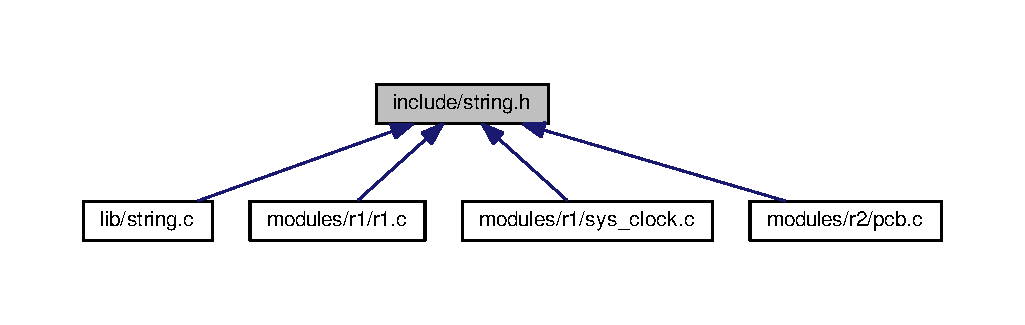
\includegraphics[width=350pt]{string_8h__dep__incl}
\end{center}
\end{figure}
\subsection*{Functions}
\begin{Indent}{\bf isspace.}\par
{\em Identifies if its space


\begin{DoxyParams}{Parameters}
{\em A} & constant character\\
\hline
\end{DoxyParams}
\begin{DoxyReturn}{Returns}
1 if it is space, otherwise return 0. 
\end{DoxyReturn}
}\begin{DoxyCompactItemize}
\item 
int {\bfseries isspace} (const char $\ast$c)\hypertarget{string_8h_a0f3d37d605e9e6d4fc1853ff9d4b91bf}{}\label{string_8h_a0f3d37d605e9e6d4fc1853ff9d4b91bf}

\end{DoxyCompactItemize}
\end{Indent}
\begin{Indent}{\bf memset.}\par
{\em Sets region of memory


\begin{DoxyParams}{Parameters}
{\em s} & destination \\
\hline
{\em c} & byte to write \\
\hline
{\em n} & count \\
\hline
\end{DoxyParams}
\begin{DoxyReturn}{Returns}
the pointer to the memory space. 
\end{DoxyReturn}
}\begin{DoxyCompactItemize}
\item 
void $\ast$ {\bfseries memset} (void $\ast$s, int c, size\+\_\+t n)\hypertarget{string_8h_ace6ee45c30e71865e6eb635200379db9}{}\label{string_8h_ace6ee45c30e71865e6eb635200379db9}

\end{DoxyCompactItemize}
\end{Indent}
\begin{Indent}{\bf \+: strcpy.}\par
{\em Copies one string to another.


\begin{DoxyParams}{Parameters}
{\em s1} & Destination string \\
\hline
{\em s2} & Source string\\
\hline
\end{DoxyParams}
\begin{DoxyReturn}{Returns}
pointer to the destination String 
\end{DoxyReturn}
}\begin{DoxyCompactItemize}
\item 
char $\ast$ {\bfseries strcpy} (char $\ast$s1, const char $\ast$s2)\hypertarget{string_8h_a1eb9cae61e6a6282c28dbc298ef7297e}{}\label{string_8h_a1eb9cae61e6a6282c28dbc298ef7297e}

\end{DoxyCompactItemize}
\end{Indent}
\begin{Indent}{\bf strcat.}\par
{\em Concatenate the contents of one string onto another.


\begin{DoxyParams}{Parameters}
{\em s1} & Destination string \\
\hline
{\em s2} & Source string \\
\hline
\end{DoxyParams}
\begin{DoxyReturn}{Returns}
pointer to destination String 
\end{DoxyReturn}
}\begin{DoxyCompactItemize}
\item 
char $\ast$ {\bfseries strcat} (char $\ast$s1, const char $\ast$s2)\hypertarget{string_8h_a8908188ae9fc2f05d993257ef001d553}{}\label{string_8h_a8908188ae9fc2f05d993257ef001d553}

\end{DoxyCompactItemize}
\end{Indent}
\begin{Indent}{\bf \+: strlen.}\par
{\em Returns the length of a string.


\begin{DoxyParams}{Parameters}
{\em s} & String input.\\
\hline
\end{DoxyParams}
\begin{DoxyReturn}{Returns}
count Length of the String 
\end{DoxyReturn}
}\begin{DoxyCompactItemize}
\item 
int {\bfseries strlen} (const char $\ast$s)\hypertarget{string_8h_a2dee044e4e667b5b789b493abd21cfa4}{}\label{string_8h_a2dee044e4e667b5b789b493abd21cfa4}

\end{DoxyCompactItemize}
\end{Indent}
\begin{Indent}{\bf \+: strcmp.}\par
{\em String comparison.


\begin{DoxyParams}{Parameters}
{\em s1} & First string to use for the compare. \\
\hline
{\em s2} & Second string to use for the compare.\\
\hline
\end{DoxyParams}
\begin{DoxyReturn}{Returns}
whether they are the same or not. 
\end{DoxyReturn}
}\begin{DoxyCompactItemize}
\item 
int {\bfseries strcmp} (const char $\ast$s1, const char $\ast$s2)\hypertarget{string_8h_a11bd144d7d44914099a3aeddf1c8567d}{}\label{string_8h_a11bd144d7d44914099a3aeddf1c8567d}

\end{DoxyCompactItemize}
\end{Indent}
\begin{Indent}{\bf strtok.}\par
{\em Split string into tokens.


\begin{DoxyParams}{Parameters}
{\em s1} & String \\
\hline
{\em s2} & Delimiter \\
\hline
\end{DoxyParams}
\begin{DoxyReturn}{Returns}
the pointer to the token. 
\end{DoxyReturn}
}\begin{DoxyCompactItemize}
\item 
char $\ast$ {\bfseries strtok} (char $\ast$s1, const char $\ast$s2)\hypertarget{string_8h_af1a867dcea42fc1215d0eddf19283ef3}{}\label{string_8h_af1a867dcea42fc1215d0eddf19283ef3}

\end{DoxyCompactItemize}
\end{Indent}
\begin{Indent}{\bf \+: atoi.}\par
{\em Convert an A\+S\+C\+II string to an integer.


\begin{DoxyParams}{Parameters}
{\em s} & String.\\
\hline
\end{DoxyParams}
\begin{DoxyReturn}{Returns}
The converted integer. 
\end{DoxyReturn}
}\begin{DoxyCompactItemize}
\item 
int {\bfseries atoi} (const char $\ast$s)\hypertarget{string_8h_a30670a60464f77af17dfb353353d6df8}{}\label{string_8h_a30670a60464f77af17dfb353353d6df8}

\end{DoxyCompactItemize}
\end{Indent}
\begin{Indent}{\bf \+: sprintf.}\par
{\em Generate a formatted string.

\%\mbox{[}-\/x\mbox{]}c output a character, \textquotesingle{}-\/\textquotesingle{} -\/ align right, x -\/ the output width

\%\mbox{[}-\/x\mbox{]}s output a string, \textquotesingle{}-\/\textquotesingle{} -\/ align right, x -\/ the output width

\%\mbox{[}\{-\/,+\}x\mbox{]}d output a character, \textquotesingle{}-\/\textquotesingle{} -\/ align right, \textquotesingle{}+\textquotesingle{} -\/ align right and display \textquotesingle{}+\textquotesingle{} sign, x -\/ the output width

\%\mbox{[}-\/x\mbox{]}X (capital \textquotesingle{}X\textquotesingle{}) output a hexadecimal number, \textquotesingle{}-\/\textquotesingle{} -\/ align right, x -\/ the output width

note\+: Output width will be ignored if width is smaller than actual length.


\begin{DoxyParams}{Parameters}
{\em str} & -\/ Output string. \\
\hline
{\em format} & -\/ The format of the string. \\
\hline
{\em ...} & -\/ All of the additional parameters. \\
\hline
\end{DoxyParams}
\begin{DoxyReturn}{Returns}
vsprintf(str, format, ap) -\/ Return the string with its format and pointer. 
\end{DoxyReturn}
}\begin{DoxyCompactItemize}
\item 
int {\bfseries sprintf} (char $\ast$str, const char $\ast$format,...)\hypertarget{string_8h_a3082155ec11e7229f7a20439b31a169e}{}\label{string_8h_a3082155ec11e7229f7a20439b31a169e}

\end{DoxyCompactItemize}
\end{Indent}
\begin{Indent}{\bf printf.}\par
{\em Print out a formatted string.

\%\mbox{[}-\/x\mbox{]}c output a character, \textquotesingle{}-\/\textquotesingle{} -\/ align right, x -\/ the output width

\%\mbox{[}-\/x\mbox{]}s output a string, \textquotesingle{}-\/\textquotesingle{} -\/ align right, x -\/ the output width

\%\mbox{[}\{-\/,+\}x\mbox{]}d output a character, \textquotesingle{}-\/\textquotesingle{} -\/ align right, \textquotesingle{}+\textquotesingle{} -\/ align right and display \textquotesingle{}+\textquotesingle{} sign, x -\/ the output width

\%\mbox{[}-\/x\mbox{]}X (capital \textquotesingle{}X\textquotesingle{}) output a hexadecimal number, \textquotesingle{}-\/\textquotesingle{} -\/ align right, x -\/ the output width

note\+: Output width will be ignored if width is smaller than actual length.


\begin{DoxyParams}{Parameters}
{\em str} & -\/ Output string. \\
\hline
{\em format} & -\/ The format of the string. \\
\hline
{\em ...} & -\/ All of the additional parameters. \\
\hline
\end{DoxyParams}
\begin{DoxyReturn}{Returns}
vsprintf(str, format, ap) -\/ Return the string with its format and pointer. 
\end{DoxyReturn}
}\begin{DoxyCompactItemize}
\item 
int {\bfseries printf} (const char $\ast$format,...)\hypertarget{string_8h_a98631211a4a8aee62f572375d5b637be}{}\label{string_8h_a98631211a4a8aee62f572375d5b637be}

\end{DoxyCompactItemize}
\end{Indent}


\subsection{Detailed Description}
Many usefull functions that used for handling string. 

\begin{DoxyAuthor}{Author}
Thunder Krakens 
\end{DoxyAuthor}
\begin{DoxyDate}{Date}
February 2nd, 2016 
\end{DoxyDate}
\begin{DoxyVersion}{Version}
R1 
\end{DoxyVersion}

\hypertarget{string_8c}{}\section{lib/string.c File Reference}
\label{string_8c}\index{lib/string.\+c@{lib/string.\+c}}


Many usefull functions that used for handling string.  


{\ttfamily \#include $<$system.\+h$>$}\\*
{\ttfamily \#include $<$core/serial.\+h$>$}\\*
{\ttfamily \#include $<$string.\+h$>$}\\*
Include dependency graph for string.\+c\+:\nopagebreak
\begin{figure}[H]
\begin{center}
\leavevmode
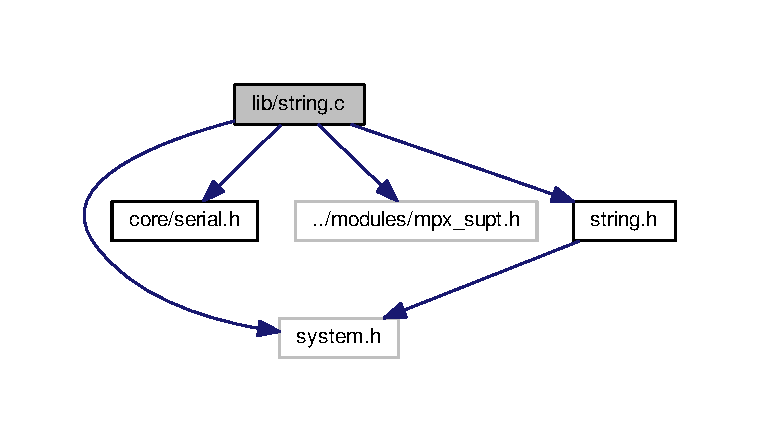
\includegraphics[width=229pt]{string_8c__incl}
\end{center}
\end{figure}
\subsection*{Functions}
\begin{Indent}{\bf strlen.}\par
{\em Returns the length of a string.


\begin{DoxyParams}{Parameters}
{\em s} & String input.\\
\hline
\end{DoxyParams}
\begin{DoxyReturn}{Returns}
count Length of the String 
\end{DoxyReturn}
}\begin{DoxyCompactItemize}
\item 
int \hyperlink{string_8c_a2dee044e4e667b5b789b493abd21cfa4}{strlen} (const char $\ast$s)
\end{DoxyCompactItemize}
\end{Indent}
\begin{Indent}{\bf strcpy.}\par
{\em Copies one string to another.


\begin{DoxyParams}{Parameters}
{\em s1} & Destination string \\
\hline
{\em s2} & Source string\\
\hline
\end{DoxyParams}
\begin{DoxyReturn}{Returns}
pointer to the destination String 
\end{DoxyReturn}
}\begin{DoxyCompactItemize}
\item 
char $\ast$ \hyperlink{string_8c_a1eb9cae61e6a6282c28dbc298ef7297e}{strcpy} (char $\ast$s1, const char $\ast$s2)
\end{DoxyCompactItemize}
\end{Indent}
\begin{Indent}{\bf atoi.}\par
{\em Convert an A\+S\+C\+II string to an integer.


\begin{DoxyParams}{Parameters}
{\em s} & String.\\
\hline
\end{DoxyParams}
\begin{DoxyReturn}{Returns}
The converted integer. 
\end{DoxyReturn}
}\begin{DoxyCompactItemize}
\item 
int \hyperlink{string_8c_a30670a60464f77af17dfb353353d6df8}{atoi} (const char $\ast$s)
\end{DoxyCompactItemize}
\end{Indent}
\begin{Indent}{\bf strcmp.}\par
{\em String comparison.


\begin{DoxyParams}{Parameters}
{\em s1} & First string to use for the compare. \\
\hline
{\em s2} & Second string to use for the compare.\\
\hline
\end{DoxyParams}
\begin{DoxyReturn}{Returns}
whether they are the same or not. 
\end{DoxyReturn}
}\begin{DoxyCompactItemize}
\item 
int \hyperlink{string_8c_a11bd144d7d44914099a3aeddf1c8567d}{strcmp} (const char $\ast$s1, const char $\ast$s2)
\end{DoxyCompactItemize}
\end{Indent}
\begin{Indent}{\bf Parse\+Padding.}\par
{\em Parse the number for padding.

(static -\/ Only can be access within this file).


\begin{DoxyParams}{Parameters}
{\em str} & Paddling String \\
\hline
{\em width} & Paddling Width \\
\hline
{\em Dec\+Width} & Width of decimal part. \\
\hline
{\em b\+Is\+Right} & Is align right. \\
\hline
{\em b\+Has\+Sign} & Has + / -\/.\\
\hline
\end{DoxyParams}
\begin{DoxyReturn}{Returns}
b\+Is\+Valid Returns the validity. 
\end{DoxyReturn}
}\end{Indent}
\begin{Indent}{\bf Add\+Pad.}\par
{\em Add a certain number of paddings (static -\/ Only can be access within this file).


\begin{DoxyParams}{Parameters}
{\em str} & In string. \\
\hline
{\em count} & Number of whitespace.\\
\hline
\end{DoxyParams}
\begin{DoxyReturn}{Returns}
V\+O\+ID 
\end{DoxyReturn}
}\end{Indent}
\begin{Indent}{\bf Nibble\+To\+Char}\par
{\em convert a nibble into a single hexadecimal (static -\/ Only can be access within this file)


\begin{DoxyParams}{Parameters}
{\em value} & The value of the nibble\\
\hline
\end{DoxyParams}
\begin{DoxyReturn}{Returns}
the character of the Hexadecimal number if valid, otherwise, return \textquotesingle{}$\ast$\textquotesingle{}. 
\end{DoxyReturn}
}\end{Indent}
\begin{Indent}{\bf bytes\+To\+Hex\+String.}\par
{\em Convert bytes into a hexadecimal string (static -\/ Only can be access within this file).


\begin{DoxyParams}{Parameters}
{\em Out\+Str} & Output string. \\
\hline
{\em Value} & The value of bytes.\\
\hline
\end{DoxyParams}
\begin{DoxyReturn}{Returns}
V\+O\+ID 
\end{DoxyReturn}
}\end{Indent}
\begin{Indent}{\bf vsprintf.}\par
{\em The actual function that perform the \char`\"{}printf\char`\"{} and \char`\"{}sprintf\char`\"{} function (static -\/ Only can be access within this file).


\begin{DoxyParams}{Parameters}
{\em str} & Output string. \\
\hline
{\em format} & The format of the string. \\
\hline
{\em ap} & the pointer of the first additional parameter.\\
\hline
\end{DoxyParams}
\begin{DoxyReturn}{Returns}
0 
\end{DoxyReturn}
}\end{Indent}
\begin{Indent}{\bf sprintf.}\par
{\em Generate a formatted string.

\%\mbox{[}-\/x\mbox{]}c output a character, \textquotesingle{}-\/\textquotesingle{} -\/ align right, x -\/ the output width

\%\mbox{[}-\/x\mbox{]}s output a string, \textquotesingle{}-\/\textquotesingle{} -\/ align right, x -\/ the output width

\%\mbox{[}\{-\/,+\}x\mbox{]}d output a character, \textquotesingle{}-\/\textquotesingle{} -\/ align right, \textquotesingle{}+\textquotesingle{} -\/ align right and display \textquotesingle{}+\textquotesingle{} sign, x -\/ the output width

\%\mbox{[}-\/x\mbox{]}X (capital \textquotesingle{}X\textquotesingle{}) output a hexadecimal number, \textquotesingle{}-\/\textquotesingle{} -\/ align right, x -\/ the output width

note\+: Output width will be ignored if width is smaller than actual length.


\begin{DoxyParams}{Parameters}
{\em str} & -\/ Output string. \\
\hline
{\em format} & -\/ The format of the string. \\
\hline
{\em ...} & -\/ All of the additional parameters. \\
\hline
\end{DoxyParams}
\begin{DoxyReturn}{Returns}
vsprintf(str, format, ap) -\/ Return the string with its format and pointer. 
\end{DoxyReturn}
}\begin{DoxyCompactItemize}
\item 
int \hyperlink{string_8c_a3082155ec11e7229f7a20439b31a169e}{sprintf} (char $\ast$str, const char $\ast$format,...)
\end{DoxyCompactItemize}
\end{Indent}
\begin{Indent}{\bf printf.}\par
{\em Print out a formatted string.

\%\mbox{[}-\/x\mbox{]}c output a character, \textquotesingle{}-\/\textquotesingle{} -\/ align right, x -\/ the output width

\%\mbox{[}-\/x\mbox{]}s output a string, \textquotesingle{}-\/\textquotesingle{} -\/ align right, x -\/ the output width

\%\mbox{[}\{-\/,+\}x\mbox{]}d output a character, \textquotesingle{}-\/\textquotesingle{} -\/ align right, \textquotesingle{}+\textquotesingle{} -\/ align right and display \textquotesingle{}+\textquotesingle{} sign, x -\/ the output width

\%\mbox{[}-\/x\mbox{]}X (capital \textquotesingle{}X\textquotesingle{}) output a hexadecimal number, \textquotesingle{}-\/\textquotesingle{} -\/ align right, x -\/ the output width

note\+: Output width will be ignored if width is smaller than actual length.


\begin{DoxyParams}{Parameters}
{\em str} & -\/ Output string. \\
\hline
{\em format} & -\/ The format of the string. \\
\hline
{\em ...} & -\/ All of the additional parameters. \\
\hline
\end{DoxyParams}
\begin{DoxyReturn}{Returns}
vsprintf(str, format, ap) -\/ Return the string with its format and pointer. 
\end{DoxyReturn}
}\begin{DoxyCompactItemize}
\item 
int \hyperlink{string_8c_a98631211a4a8aee62f572375d5b637be}{printf} (const char $\ast$format,...)
\item 
char $\ast$ \hyperlink{string_8c_a8908188ae9fc2f05d993257ef001d553}{strcat} (char $\ast$s1, const char $\ast$s2)
\item 
int \hyperlink{string_8c_a0f3d37d605e9e6d4fc1853ff9d4b91bf}{isspace} (const char $\ast$c)
\item 
void $\ast$ \hyperlink{string_8c_ace6ee45c30e71865e6eb635200379db9}{memset} (void $\ast$s, int c, size\+\_\+t n)
\item 
char $\ast$ \hyperlink{string_8c_af1a867dcea42fc1215d0eddf19283ef3}{strtok} (char $\ast$s1, const char $\ast$s2)
\end{DoxyCompactItemize}
\end{Indent}


\subsection{Detailed Description}
Many usefull functions that used for handling string. 

\begin{DoxyAuthor}{Author}
Thunder Krakens 
\end{DoxyAuthor}
\begin{DoxyDate}{Date}
February 2nd, 2016 
\end{DoxyDate}
\begin{DoxyVersion}{Version}
R1 
\end{DoxyVersion}


\subsection{Function Documentation}
\index{string.\+c@{string.\+c}!atoi@{atoi}}
\index{atoi@{atoi}!string.\+c@{string.\+c}}
\subsubsection[{\texorpdfstring{atoi(const char $\ast$s)}{atoi(const char *s)}}]{\setlength{\rightskip}{0pt plus 5cm}int atoi (
\begin{DoxyParamCaption}
\item[{const char $\ast$}]{s}
\end{DoxyParamCaption}
)}\hypertarget{string_8c_a30670a60464f77af17dfb353353d6df8}{}\label{string_8c_a30670a60464f77af17dfb353353d6df8}


Here is the call graph for this function\+:\nopagebreak
\begin{figure}[H]
\begin{center}
\leavevmode
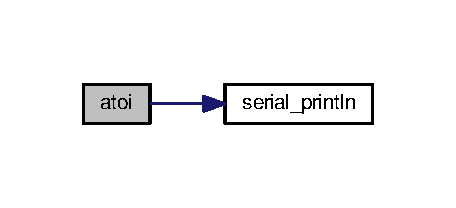
\includegraphics[width=219pt]{string_8c_a30670a60464f77af17dfb353353d6df8_cgraph}
\end{center}
\end{figure}




Here is the caller graph for this function\+:
\nopagebreak
\begin{figure}[H]
\begin{center}
\leavevmode
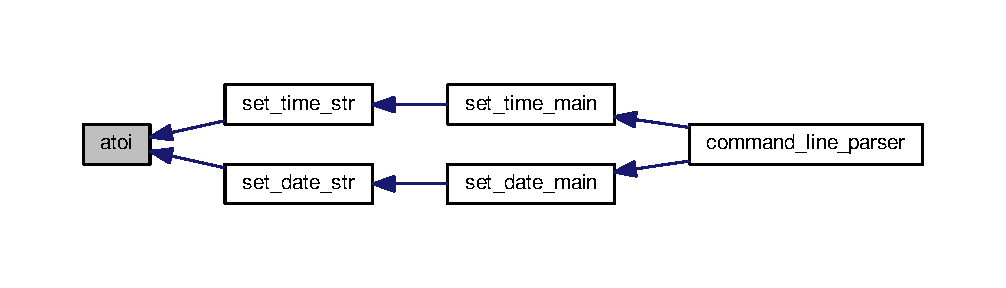
\includegraphics[width=350pt]{string_8c_a30670a60464f77af17dfb353353d6df8_icgraph}
\end{center}
\end{figure}


\index{string.\+c@{string.\+c}!isspace@{isspace}}
\index{isspace@{isspace}!string.\+c@{string.\+c}}
\subsubsection[{\texorpdfstring{isspace(const char $\ast$c)}{isspace(const char *c)}}]{\setlength{\rightskip}{0pt plus 5cm}int isspace (
\begin{DoxyParamCaption}
\item[{const char $\ast$}]{c}
\end{DoxyParamCaption}
)}\hypertarget{string_8c_a0f3d37d605e9e6d4fc1853ff9d4b91bf}{}\label{string_8c_a0f3d37d605e9e6d4fc1853ff9d4b91bf}
\index{string.\+c@{string.\+c}!memset@{memset}}
\index{memset@{memset}!string.\+c@{string.\+c}}
\subsubsection[{\texorpdfstring{memset(void $\ast$s, int c, size\+\_\+t n)}{memset(void *s, int c, size_t n)}}]{\setlength{\rightskip}{0pt plus 5cm}void$\ast$ memset (
\begin{DoxyParamCaption}
\item[{void $\ast$}]{s, }
\item[{int}]{c, }
\item[{size\+\_\+t}]{n}
\end{DoxyParamCaption}
)}\hypertarget{string_8c_ace6ee45c30e71865e6eb635200379db9}{}\label{string_8c_ace6ee45c30e71865e6eb635200379db9}


Here is the caller graph for this function\+:
\nopagebreak
\begin{figure}[H]
\begin{center}
\leavevmode
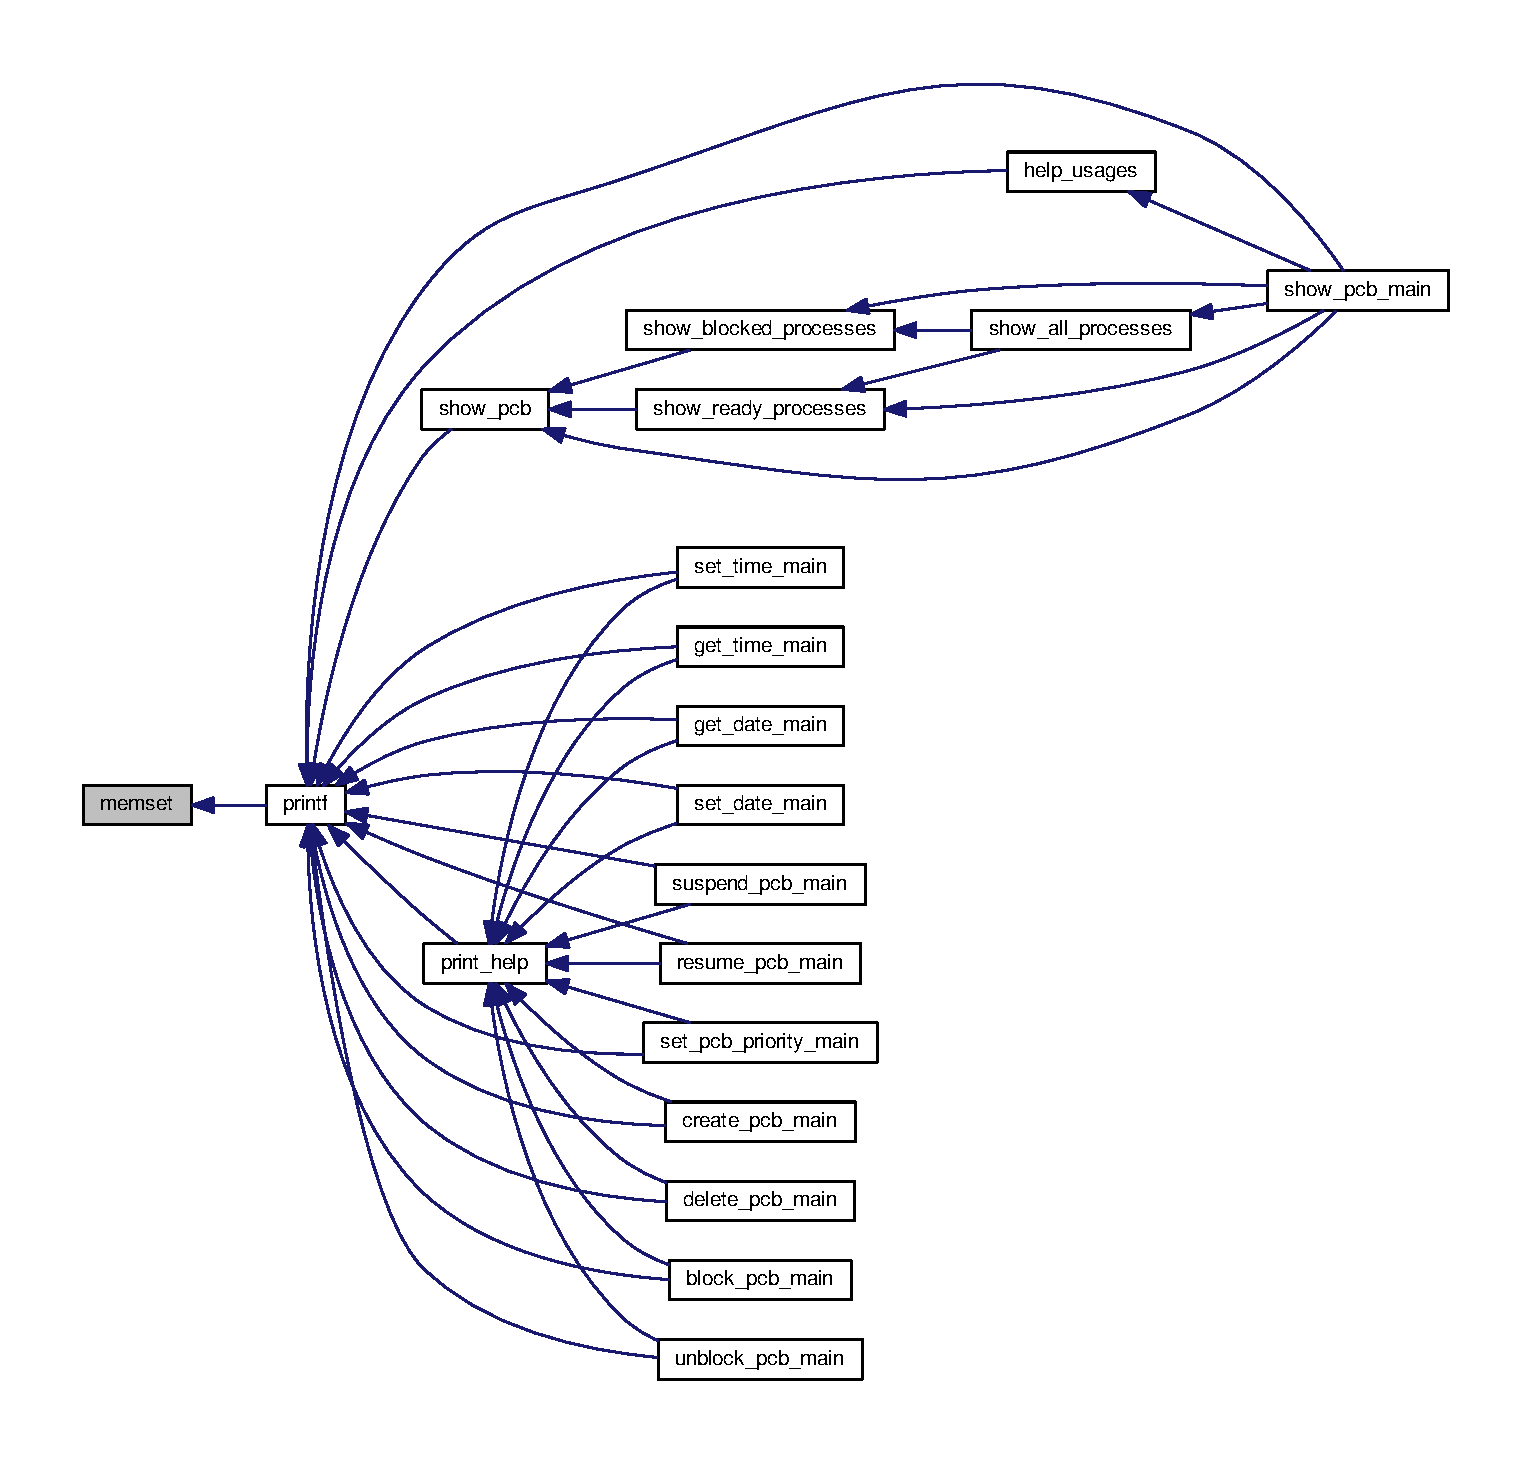
\includegraphics[width=350pt]{string_8c_ace6ee45c30e71865e6eb635200379db9_icgraph}
\end{center}
\end{figure}


\index{string.\+c@{string.\+c}!printf@{printf}}
\index{printf@{printf}!string.\+c@{string.\+c}}
\subsubsection[{\texorpdfstring{printf(const char $\ast$format,...)}{printf(const char *format,...)}}]{\setlength{\rightskip}{0pt plus 5cm}int printf (
\begin{DoxyParamCaption}
\item[{const char $\ast$}]{format, }
\item[{}]{...}
\end{DoxyParamCaption}
)}\hypertarget{string_8c_a98631211a4a8aee62f572375d5b637be}{}\label{string_8c_a98631211a4a8aee62f572375d5b637be}


Here is the call graph for this function\+:\nopagebreak
\begin{figure}[H]
\begin{center}
\leavevmode
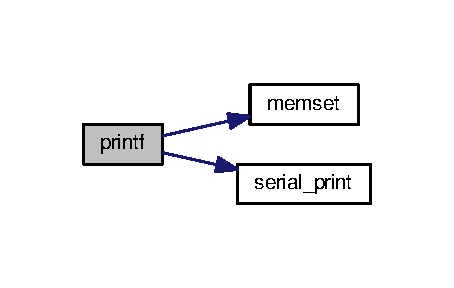
\includegraphics[width=218pt]{string_8c_a98631211a4a8aee62f572375d5b637be_cgraph}
\end{center}
\end{figure}




Here is the caller graph for this function\+:
\nopagebreak
\begin{figure}[H]
\begin{center}
\leavevmode
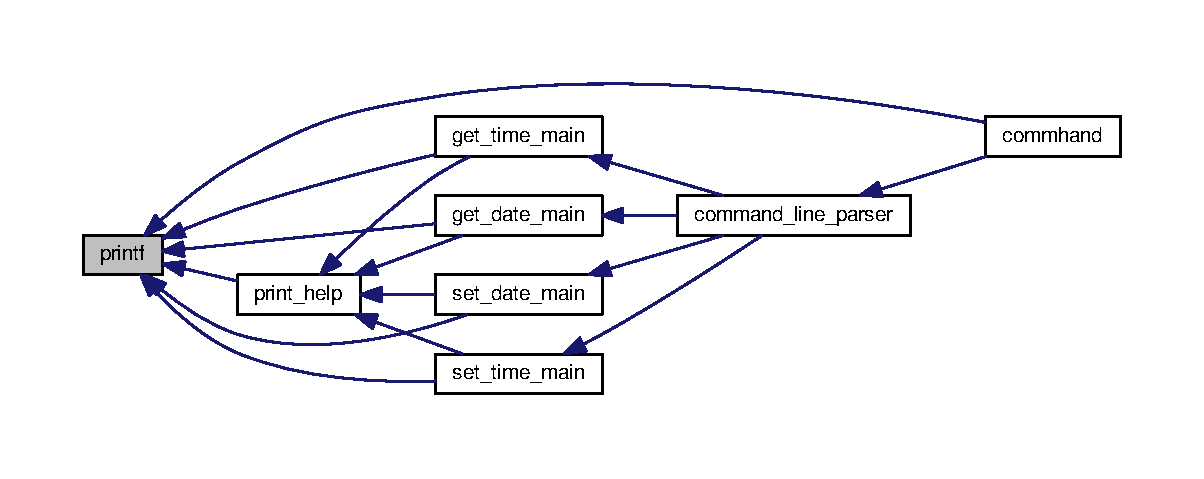
\includegraphics[width=350pt]{string_8c_a98631211a4a8aee62f572375d5b637be_icgraph}
\end{center}
\end{figure}


\index{string.\+c@{string.\+c}!sprintf@{sprintf}}
\index{sprintf@{sprintf}!string.\+c@{string.\+c}}
\subsubsection[{\texorpdfstring{sprintf(char $\ast$str, const char $\ast$format,...)}{sprintf(char *str, const char *format,...)}}]{\setlength{\rightskip}{0pt plus 5cm}int sprintf (
\begin{DoxyParamCaption}
\item[{char $\ast$}]{str, }
\item[{const char $\ast$}]{format, }
\item[{}]{...}
\end{DoxyParamCaption}
)}\hypertarget{string_8c_a3082155ec11e7229f7a20439b31a169e}{}\label{string_8c_a3082155ec11e7229f7a20439b31a169e}
\index{string.\+c@{string.\+c}!strcat@{strcat}}
\index{strcat@{strcat}!string.\+c@{string.\+c}}
\subsubsection[{\texorpdfstring{strcat(char $\ast$s1, const char $\ast$s2)}{strcat(char *s1, const char *s2)}}]{\setlength{\rightskip}{0pt plus 5cm}char$\ast$ strcat (
\begin{DoxyParamCaption}
\item[{char $\ast$}]{s1, }
\item[{const char $\ast$}]{s2}
\end{DoxyParamCaption}
)}\hypertarget{string_8c_a8908188ae9fc2f05d993257ef001d553}{}\label{string_8c_a8908188ae9fc2f05d993257ef001d553}


Here is the caller graph for this function\+:
\nopagebreak
\begin{figure}[H]
\begin{center}
\leavevmode
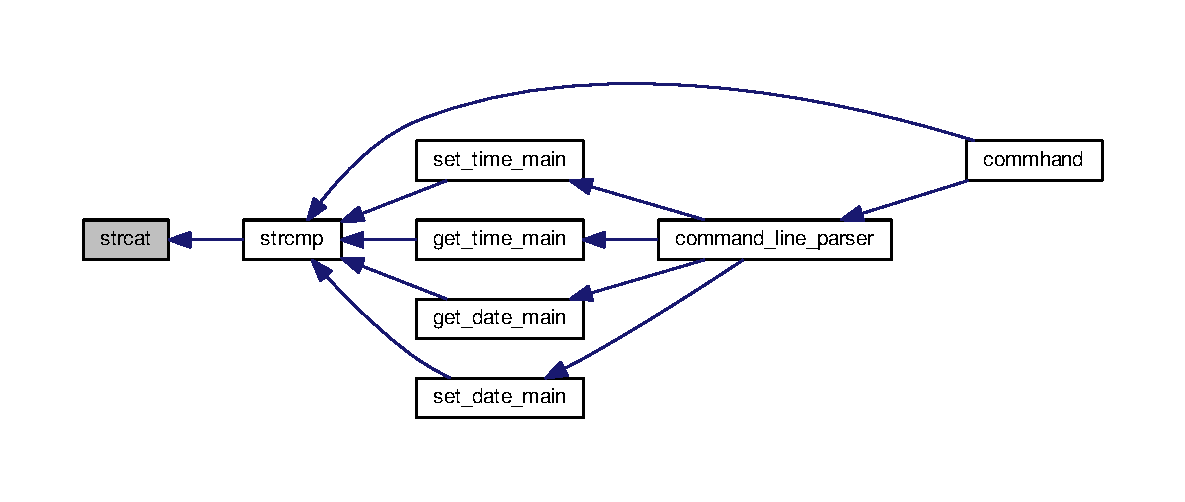
\includegraphics[width=350pt]{string_8c_a8908188ae9fc2f05d993257ef001d553_icgraph}
\end{center}
\end{figure}


\index{string.\+c@{string.\+c}!strcmp@{strcmp}}
\index{strcmp@{strcmp}!string.\+c@{string.\+c}}
\subsubsection[{\texorpdfstring{strcmp(const char $\ast$s1, const char $\ast$s2)}{strcmp(const char *s1, const char *s2)}}]{\setlength{\rightskip}{0pt plus 5cm}int strcmp (
\begin{DoxyParamCaption}
\item[{const char $\ast$}]{s1, }
\item[{const char $\ast$}]{s2}
\end{DoxyParamCaption}
)}\hypertarget{string_8c_a11bd144d7d44914099a3aeddf1c8567d}{}\label{string_8c_a11bd144d7d44914099a3aeddf1c8567d}


Here is the call graph for this function\+:\nopagebreak
\begin{figure}[H]
\begin{center}
\leavevmode
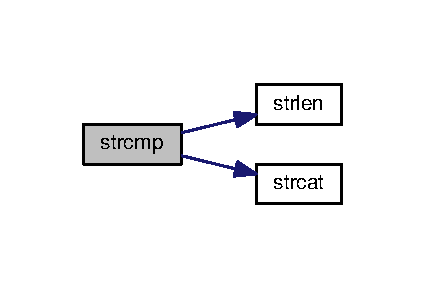
\includegraphics[width=204pt]{string_8c_a11bd144d7d44914099a3aeddf1c8567d_cgraph}
\end{center}
\end{figure}




Here is the caller graph for this function\+:
\nopagebreak
\begin{figure}[H]
\begin{center}
\leavevmode
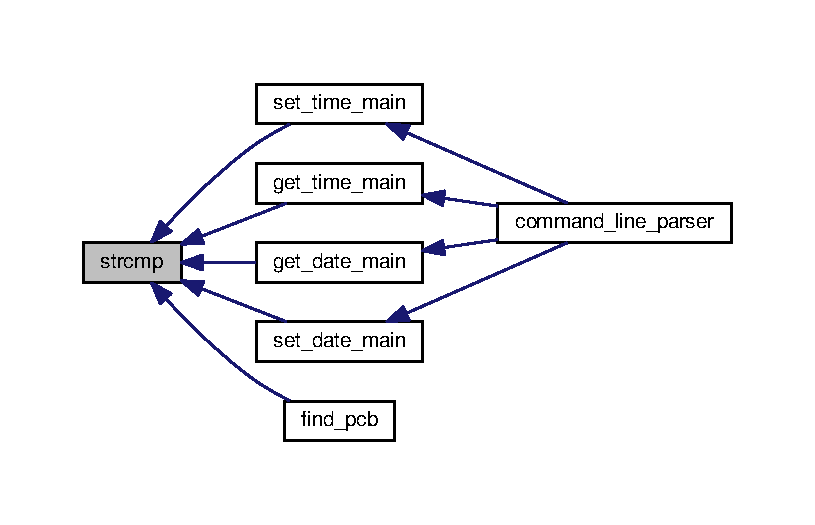
\includegraphics[width=350pt]{string_8c_a11bd144d7d44914099a3aeddf1c8567d_icgraph}
\end{center}
\end{figure}


\index{string.\+c@{string.\+c}!strcpy@{strcpy}}
\index{strcpy@{strcpy}!string.\+c@{string.\+c}}
\subsubsection[{\texorpdfstring{strcpy(char $\ast$s1, const char $\ast$s2)}{strcpy(char *s1, const char *s2)}}]{\setlength{\rightskip}{0pt plus 5cm}char$\ast$ strcpy (
\begin{DoxyParamCaption}
\item[{char $\ast$}]{s1, }
\item[{const char $\ast$}]{s2}
\end{DoxyParamCaption}
)}\hypertarget{string_8c_a1eb9cae61e6a6282c28dbc298ef7297e}{}\label{string_8c_a1eb9cae61e6a6282c28dbc298ef7297e}


Here is the caller graph for this function\+:
\nopagebreak
\begin{figure}[H]
\begin{center}
\leavevmode
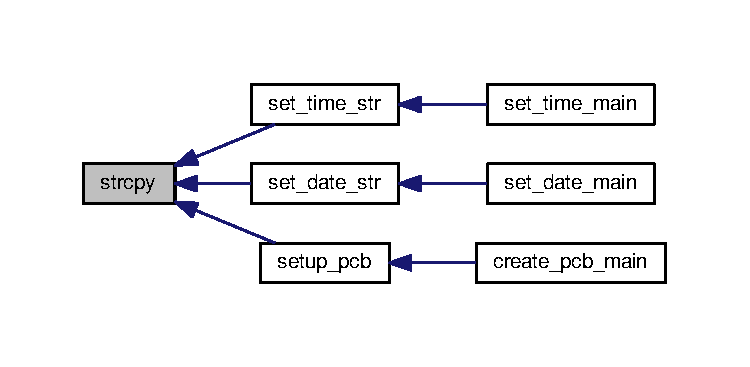
\includegraphics[width=350pt]{string_8c_a1eb9cae61e6a6282c28dbc298ef7297e_icgraph}
\end{center}
\end{figure}


\index{string.\+c@{string.\+c}!strlen@{strlen}}
\index{strlen@{strlen}!string.\+c@{string.\+c}}
\subsubsection[{\texorpdfstring{strlen(const char $\ast$s)}{strlen(const char *s)}}]{\setlength{\rightskip}{0pt plus 5cm}int strlen (
\begin{DoxyParamCaption}
\item[{const char $\ast$}]{s}
\end{DoxyParamCaption}
)}\hypertarget{string_8c_a2dee044e4e667b5b789b493abd21cfa4}{}\label{string_8c_a2dee044e4e667b5b789b493abd21cfa4}


Here is the caller graph for this function\+:
\nopagebreak
\begin{figure}[H]
\begin{center}
\leavevmode
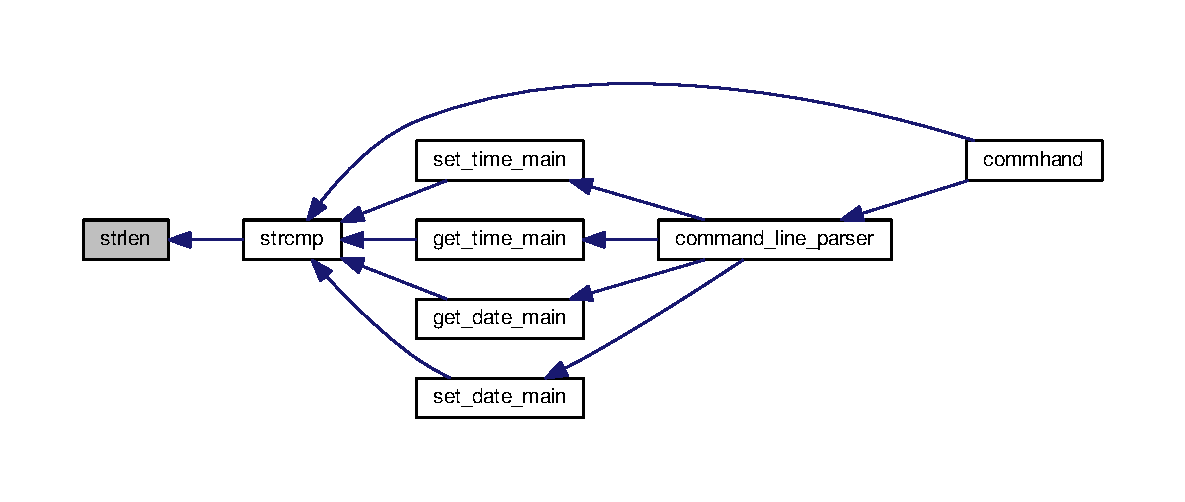
\includegraphics[width=350pt]{string_8c_a2dee044e4e667b5b789b493abd21cfa4_icgraph}
\end{center}
\end{figure}


\index{string.\+c@{string.\+c}!strtok@{strtok}}
\index{strtok@{strtok}!string.\+c@{string.\+c}}
\subsubsection[{\texorpdfstring{strtok(char $\ast$s1, const char $\ast$s2)}{strtok(char *s1, const char *s2)}}]{\setlength{\rightskip}{0pt plus 5cm}char$\ast$ strtok (
\begin{DoxyParamCaption}
\item[{char $\ast$}]{s1, }
\item[{const char $\ast$}]{s2}
\end{DoxyParamCaption}
)}\hypertarget{string_8c_af1a867dcea42fc1215d0eddf19283ef3}{}\label{string_8c_af1a867dcea42fc1215d0eddf19283ef3}


Here is the caller graph for this function\+:
\nopagebreak
\begin{figure}[H]
\begin{center}
\leavevmode
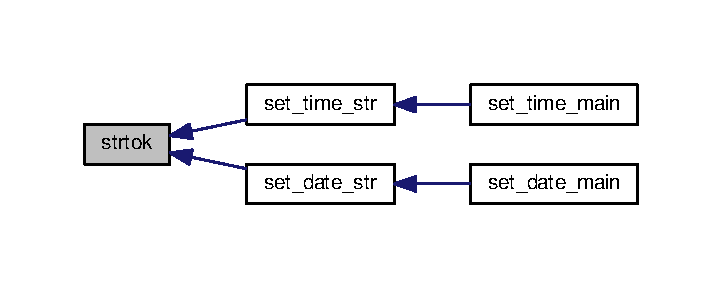
\includegraphics[width=350pt]{string_8c_af1a867dcea42fc1215d0eddf19283ef3_icgraph}
\end{center}
\end{figure}



\hypertarget{errno_8h}{\section{modules/errno.h File Reference}
\label{errno_8h}\index{modules/errno.\-h@{modules/errno.\-h}}
}


This file contains the type of errors. The error can be from invalid paramter passed to a function, or invalid input format.  


This graph shows which files directly or indirectly include this file\-:\nopagebreak
\begin{figure}[H]
\begin{center}
\leavevmode
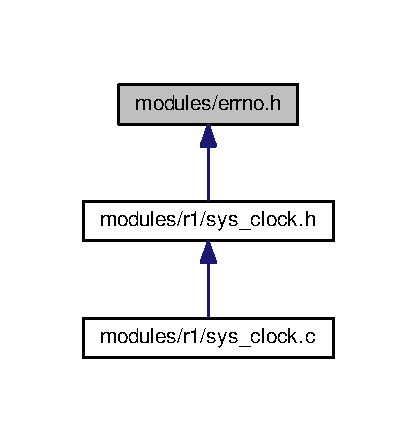
\includegraphics[width=350pt]{errno_8h__dep__incl}
\end{center}
\end{figure}
\subsection*{Macros}
\begin{DoxyCompactItemize}
\item 
\#define \hyperlink{errno_8h_a910656a3ce04eecb0e4479fd35d343fb}{E\-\_\-\-N\-O\-E\-R\-R\-O\-R}~0
\item 
\#define \hyperlink{errno_8h_ad38311f7eadb9042f7c98dd31ffc69c3}{E\-\_\-\-I\-N\-V\-P\-A\-R\-A}~1
\item 
\#define \hyperlink{errno_8h_a17ad8897d139d58bb84714b2e7861ba2}{E\-\_\-\-I\-N\-V\-S\-T\-R\-F}~2
\item 
\#define \hyperlink{errno_8h_a5273e7742dd7c18937e5191b8070f08f}{E\-\_\-\-I\-N\-V\-U\-S\-R\-I}~3
\item 
\#define \hyperlink{errno_8h_a7fcfdab3c40ca9d8eb249d636908c3fd}{E\-\_\-\-F\-R\-E\-E\-M\-E\-M}~4
\begin{DoxyCompactList}\small\item\em Error we cannot actually free the memory space since the student\-\_\-free had not been implemented before R5. \end{DoxyCompactList}\item 
\#define \hyperlink{errno_8h_a97fcdfde06438bcf94181400389bd7b9}{E\-\_\-\-N\-U\-L\-L\-\_\-\-P\-T\-R}~5
\begin{DoxyCompactList}\small\item\em A N\-U\-L\-L Pointer Error. \end{DoxyCompactList}\item 
\#define \hyperlink{errno_8h_af40255ba5e6a1e879803d699b4393cac}{E\-\_\-\-P\-R\-O\-G\-E\-R\-R}~99
\end{DoxyCompactItemize}
\subsection*{Typedefs}
\begin{Indent}{\bf error\-\_\-t.}\par
{\em The datetype that holds the error code. }\begin{DoxyCompactItemize}
\item 
typedef unsigned int \hyperlink{errno_8h_aafbeb34410283829794b35fedafeb369}{error\-\_\-t}
\end{DoxyCompactItemize}
\end{Indent}


\subsection{Detailed Description}
This file contains the type of errors. The error can be from invalid paramter passed to a function, or invalid input format. \begin{DoxyAuthor}{Author}
Thunder Krakens 
\end{DoxyAuthor}
\begin{DoxyDate}{Date}
February 7nd, 2016 
\end{DoxyDate}
\begin{DoxyVersion}{Version}
R2 
\end{DoxyVersion}


\subsection{Macro Definition Documentation}
\hypertarget{errno_8h_a7fcfdab3c40ca9d8eb249d636908c3fd}{\index{errno.\-h@{errno.\-h}!E\-\_\-\-F\-R\-E\-E\-M\-E\-M@{E\-\_\-\-F\-R\-E\-E\-M\-E\-M}}
\index{E\-\_\-\-F\-R\-E\-E\-M\-E\-M@{E\-\_\-\-F\-R\-E\-E\-M\-E\-M}!errno.h@{errno.\-h}}
\subsubsection[{E\-\_\-\-F\-R\-E\-E\-M\-E\-M}]{\setlength{\rightskip}{0pt plus 5cm}\#define E\-\_\-\-F\-R\-E\-E\-M\-E\-M~4}}\label{errno_8h_a7fcfdab3c40ca9d8eb249d636908c3fd}


Error we cannot actually free the memory space since the student\-\_\-free had not been implemented before R5. 

\hypertarget{errno_8h_ad38311f7eadb9042f7c98dd31ffc69c3}{\index{errno.\-h@{errno.\-h}!E\-\_\-\-I\-N\-V\-P\-A\-R\-A@{E\-\_\-\-I\-N\-V\-P\-A\-R\-A}}
\index{E\-\_\-\-I\-N\-V\-P\-A\-R\-A@{E\-\_\-\-I\-N\-V\-P\-A\-R\-A}!errno.h@{errno.\-h}}
\subsubsection[{E\-\_\-\-I\-N\-V\-P\-A\-R\-A}]{\setlength{\rightskip}{0pt plus 5cm}\#define E\-\_\-\-I\-N\-V\-P\-A\-R\-A~1}}\label{errno_8h_ad38311f7eadb9042f7c98dd31ffc69c3}
\hypertarget{errno_8h_a17ad8897d139d58bb84714b2e7861ba2}{\index{errno.\-h@{errno.\-h}!E\-\_\-\-I\-N\-V\-S\-T\-R\-F@{E\-\_\-\-I\-N\-V\-S\-T\-R\-F}}
\index{E\-\_\-\-I\-N\-V\-S\-T\-R\-F@{E\-\_\-\-I\-N\-V\-S\-T\-R\-F}!errno.h@{errno.\-h}}
\subsubsection[{E\-\_\-\-I\-N\-V\-S\-T\-R\-F}]{\setlength{\rightskip}{0pt plus 5cm}\#define E\-\_\-\-I\-N\-V\-S\-T\-R\-F~2}}\label{errno_8h_a17ad8897d139d58bb84714b2e7861ba2}
\hypertarget{errno_8h_a5273e7742dd7c18937e5191b8070f08f}{\index{errno.\-h@{errno.\-h}!E\-\_\-\-I\-N\-V\-U\-S\-R\-I@{E\-\_\-\-I\-N\-V\-U\-S\-R\-I}}
\index{E\-\_\-\-I\-N\-V\-U\-S\-R\-I@{E\-\_\-\-I\-N\-V\-U\-S\-R\-I}!errno.h@{errno.\-h}}
\subsubsection[{E\-\_\-\-I\-N\-V\-U\-S\-R\-I}]{\setlength{\rightskip}{0pt plus 5cm}\#define E\-\_\-\-I\-N\-V\-U\-S\-R\-I~3}}\label{errno_8h_a5273e7742dd7c18937e5191b8070f08f}
\hypertarget{errno_8h_a910656a3ce04eecb0e4479fd35d343fb}{\index{errno.\-h@{errno.\-h}!E\-\_\-\-N\-O\-E\-R\-R\-O\-R@{E\-\_\-\-N\-O\-E\-R\-R\-O\-R}}
\index{E\-\_\-\-N\-O\-E\-R\-R\-O\-R@{E\-\_\-\-N\-O\-E\-R\-R\-O\-R}!errno.h@{errno.\-h}}
\subsubsection[{E\-\_\-\-N\-O\-E\-R\-R\-O\-R}]{\setlength{\rightskip}{0pt plus 5cm}\#define E\-\_\-\-N\-O\-E\-R\-R\-O\-R~0}}\label{errno_8h_a910656a3ce04eecb0e4479fd35d343fb}
\hypertarget{errno_8h_a97fcdfde06438bcf94181400389bd7b9}{\index{errno.\-h@{errno.\-h}!E\-\_\-\-N\-U\-L\-L\-\_\-\-P\-T\-R@{E\-\_\-\-N\-U\-L\-L\-\_\-\-P\-T\-R}}
\index{E\-\_\-\-N\-U\-L\-L\-\_\-\-P\-T\-R@{E\-\_\-\-N\-U\-L\-L\-\_\-\-P\-T\-R}!errno.h@{errno.\-h}}
\subsubsection[{E\-\_\-\-N\-U\-L\-L\-\_\-\-P\-T\-R}]{\setlength{\rightskip}{0pt plus 5cm}\#define E\-\_\-\-N\-U\-L\-L\-\_\-\-P\-T\-R~5}}\label{errno_8h_a97fcdfde06438bcf94181400389bd7b9}


A N\-U\-L\-L Pointer Error. 

\hypertarget{errno_8h_af40255ba5e6a1e879803d699b4393cac}{\index{errno.\-h@{errno.\-h}!E\-\_\-\-P\-R\-O\-G\-E\-R\-R@{E\-\_\-\-P\-R\-O\-G\-E\-R\-R}}
\index{E\-\_\-\-P\-R\-O\-G\-E\-R\-R@{E\-\_\-\-P\-R\-O\-G\-E\-R\-R}!errno.h@{errno.\-h}}
\subsubsection[{E\-\_\-\-P\-R\-O\-G\-E\-R\-R}]{\setlength{\rightskip}{0pt plus 5cm}\#define E\-\_\-\-P\-R\-O\-G\-E\-R\-R~99}}\label{errno_8h_af40255ba5e6a1e879803d699b4393cac}


\subsection{Typedef Documentation}
\hypertarget{errno_8h_aafbeb34410283829794b35fedafeb369}{\index{errno.\-h@{errno.\-h}!error\-\_\-t@{error\-\_\-t}}
\index{error\-\_\-t@{error\-\_\-t}!errno.h@{errno.\-h}}
\subsubsection[{error\-\_\-t}]{\setlength{\rightskip}{0pt plus 5cm}typedef unsigned int {\bf error\-\_\-t}}}\label{errno_8h_aafbeb34410283829794b35fedafeb369}

\hypertarget{r1_8c}{}\section{modules/r1/r1.c File Reference}
\label{r1_8c}\index{modules/r1/r1.\+c@{modules/r1/r1.\+c}}


The main code file for Module R1.  


{\ttfamily \#include \char`\"{}r1.\+h\char`\"{}}\\*
{\ttfamily \#include \char`\"{}../mpx\+\_\+supt.\+h\char`\"{}}\\*
{\ttfamily \#include \char`\"{}sys\+\_\+clock.\+h\char`\"{}}\\*
{\ttfamily \#include $<$string.\+h$>$}\\*
{\ttfamily \#include $<$core/serial.\+h$>$}\\*
{\ttfamily \#include $<$core/io.\+h$>$}\\*
\subsection*{Macros}
\begin{DoxyCompactItemize}
\item 
\#define {\bfseries U\+S\+E\+R\+\_\+\+I\+N\+P\+U\+T\+\_\+\+B\+U\+F\+F\+E\+R\+\_\+\+S\+I\+ZE}~1000\hypertarget{r1_8c_abcc7a443a9849435cd308e774dd0c8de}{}\label{r1_8c_abcc7a443a9849435cd308e774dd0c8de}

\item 
\#define {\bfseries M\+A\+X\+\_\+\+A\+R\+GC}~50\hypertarget{r1_8c_ae1da50c0d24fa0390a6c287d6cb4befe}{}\label{r1_8c_ae1da50c0d24fa0390a6c287d6cb4befe}

\item 
\#define {\bfseries M\+O\+D\+\_\+\+V\+E\+R\+S\+I\+ON}~\char`\"{}R1\char`\"{}\hypertarget{r1_8c_a88a929d879ebd5f0d64773050f62aef5}{}\label{r1_8c_a88a929d879ebd5f0d64773050f62aef5}

\item 
\#define {\bfseries C\+O\+M\+P\+L\+E\+T\+I\+ON}~\char`\"{}02/05/2016\char`\"{}\hypertarget{r1_8c_afc29c35952a1ce914016dbfa4b91c2aa}{}\label{r1_8c_afc29c35952a1ce914016dbfa4b91c2aa}

\end{DoxyCompactItemize}
\subsection*{Enumerations}
\begin{DoxyCompactItemize}
\item 
enum \hyperlink{r1_8c_abb950b1df1e3f5562228a4eae8ebb925}{Command\+Paser\+Stat} \{ {\bfseries Not\+Writing}, 
{\bfseries Normal\+Writing}, 
{\bfseries Double\+Quote\+Writing}, 
{\bfseries Single\+Quote\+Writing}
 \}\begin{DoxyCompactList}\small\item\em Name\+: Command\+Parser\+Stat. \end{DoxyCompactList}
\end{DoxyCompactItemize}
\subsection*{Functions}
\begin{DoxyCompactItemize}
\item 
int \hyperlink{r1_8c_a14d85617242501c323a203ee196d3efa}{commhand} ()
\begin{DoxyCompactList}\small\item\em Name\+: commhand. \end{DoxyCompactList}\item 
void \hyperlink{r1_8c_adb6b307c73bca25d17aa7683e14fea16}{command\+\_\+line\+\_\+parser} (const char $\ast$Cmd\+Str, int $\ast$argc, char $\ast$$\ast$argv, const int Max\+Arg\+Num, const int Max\+Str\+Len)
\begin{DoxyCompactList}\small\item\em Name\+: command\+\_\+line\+\_\+parser. \end{DoxyCompactList}\end{DoxyCompactItemize}


\subsection{Detailed Description}
The main code file for Module R1. 

\begin{DoxyAuthor}{Author}
Thunder Krakens 
\end{DoxyAuthor}
\begin{DoxyDate}{Date}
February 2nd, 2016 
\end{DoxyDate}
\begin{DoxyVersion}{Version}
R1
\end{DoxyVersion}
This file contains setdate, getdate, settime, gettime, help functions, commandhander and command line parser 

\subsection{Enumeration Type Documentation}
\index{r1.\+c@{r1.\+c}!Command\+Paser\+Stat@{Command\+Paser\+Stat}}
\index{Command\+Paser\+Stat@{Command\+Paser\+Stat}!r1.\+c@{r1.\+c}}
\subsubsection[{\texorpdfstring{Command\+Paser\+Stat}{CommandPaserStat}}]{\setlength{\rightskip}{0pt plus 5cm}enum {\bf Command\+Paser\+Stat}}\hypertarget{r1_8c_abb950b1df1e3f5562228a4eae8ebb925}{}\label{r1_8c_abb950b1df1e3f5562228a4eae8ebb925}


Name\+: Command\+Parser\+Stat. 

Description\+: The stats of the command parser 

\subsection{Function Documentation}
\index{r1.\+c@{r1.\+c}!command\+\_\+line\+\_\+parser@{command\+\_\+line\+\_\+parser}}
\index{command\+\_\+line\+\_\+parser@{command\+\_\+line\+\_\+parser}!r1.\+c@{r1.\+c}}
\subsubsection[{\texorpdfstring{command\+\_\+line\+\_\+parser(const char $\ast$\+Cmd\+Str, int $\ast$argc, char $\ast$$\ast$argv, const int Max\+Arg\+Num, const int Max\+Str\+Len)}{command_line_parser(const char *CmdStr, int *argc, char **argv, const int MaxArgNum, const int MaxStrLen)}}]{\setlength{\rightskip}{0pt plus 5cm}void command\+\_\+line\+\_\+parser (
\begin{DoxyParamCaption}
\item[{const char $\ast$}]{Cmd\+Str, }
\item[{int $\ast$}]{argc, }
\item[{char $\ast$$\ast$}]{argv, }
\item[{const int}]{Max\+Arg\+Num, }
\item[{const int}]{Max\+Str\+Len}
\end{DoxyParamCaption}
)}\hypertarget{r1_8c_adb6b307c73bca25d17aa7683e14fea16}{}\label{r1_8c_adb6b307c73bca25d17aa7683e14fea16}


Name\+: command\+\_\+line\+\_\+parser. 

Description\+: Splits the complete command line into tokens by space, single quote, or double quote.


\begin{DoxyParams}{Parameters}
{\em Cmd\+Str} & -\/ The complete input command. \\
\hline
{\em argc} & -\/ The number of tokens found. \\
\hline
{\em argv} & -\/ The array of tokens. \\
\hline
{\em Max\+Arg\+Num} & -\/ The maximum number of tokens that array can hold. \\
\hline
{\em Max\+Str\+Len} & -\/ The maximum length of each token that string can hold.\\
\hline
\end{DoxyParams}
\begin{DoxyReturn}{Returns}
void 
\end{DoxyReturn}
\index{r1.\+c@{r1.\+c}!commhand@{commhand}}
\index{commhand@{commhand}!r1.\+c@{r1.\+c}}
\subsubsection[{\texorpdfstring{commhand()}{commhand()}}]{\setlength{\rightskip}{0pt plus 5cm}int commhand (
\begin{DoxyParamCaption}
{}
\end{DoxyParamCaption}
)}\hypertarget{r1_8c_a14d85617242501c323a203ee196d3efa}{}\label{r1_8c_a14d85617242501c323a203ee196d3efa}


Name\+: commhand. 

Description\+: Accepts and handles commands from the user. 
\begin{DoxyParams}{Parameters}
{\em User} & input \\
\hline
\end{DoxyParams}
\begin{DoxyReturn}{Returns}
0 
\end{DoxyReturn}

\hypertarget{r1_8h}{}\section{modules/r1/r1.h File Reference}
\label{r1_8h}\index{modules/r1/r1.\+h@{modules/r1/r1.\+h}}


The commandhander and functions associations for Module R1.  


This graph shows which files directly or indirectly include this file\+:\nopagebreak
\begin{figure}[H]
\begin{center}
\leavevmode
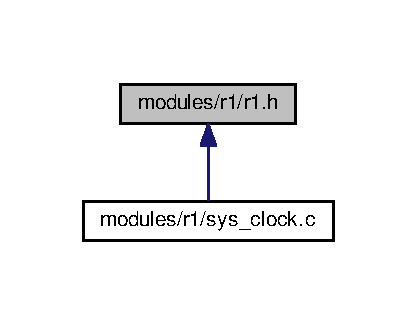
\includegraphics[width=302pt]{r1_8h__dep__incl}
\end{center}
\end{figure}
\subsection*{Macros}
\begin{DoxyCompactItemize}
\item 
\#define \hyperlink{r1_8h_ae8a798ec5e0449028e485688e8241b5e}{H\+E\+LP}~0
\item 
\#define \hyperlink{r1_8h_a1c6d5de492ac61ad29aec7aa9a436bbf}{V\+E\+R\+S\+I\+ON}~1
\item 
\#define \hyperlink{r1_8h_ab1586d6a1539e7921374aeea8b907805}{G\+E\+T\+T\+I\+ME}~2
\item 
\#define \hyperlink{r1_8h_a27a942da2560b15dc5291c8f386c426a}{S\+E\+T\+T\+I\+ME}~3
\item 
\#define \hyperlink{r1_8h_a6ec5835e6ff9d5af0a3a1996746ee5b9}{G\+E\+T\+D\+A\+TE}~4
\item 
\#define \hyperlink{r1_8h_ac1f0ac55b810f16f95393b27e9780bf3}{S\+E\+T\+D\+A\+TE}~5
\item 
\#define \hyperlink{r1_8h_a3b61478edd7c1b25c8facd2907cf6c33}{S\+H\+U\+T\+D\+O\+WN}~6
\item 
\#define \hyperlink{r1_8h_a8e8928373d15397e25be8ecb76c727da}{N\+U\+M\+\_\+\+O\+F\+\_\+\+F\+U\+N\+C\+T\+I\+O\+NS}~7
\end{DoxyCompactItemize}
\subsection*{Functions}
\begin{Indent}{\bf commhand}\par
{\em Accepts and handles commands from the user.

\begin{DoxyReturn}{Returns}
0 
\end{DoxyReturn}
}\begin{DoxyCompactItemize}
\item 
int \hyperlink{r1_8h_a14d85617242501c323a203ee196d3efa}{commhand} ()
\end{DoxyCompactItemize}
\end{Indent}
\begin{Indent}{\bf command\+\_\+line\+\_\+parser}\par
{\em Splits the complete command line into tokens by space, single quote, or double quote.


\begin{DoxyParams}{Parameters}
{\em Cmd\+Str} & The complete input command. \\
\hline
{\em argc} & The number of tokens found. \\
\hline
{\em argv} & The array of tokens. \\
\hline
{\em Max\+Arg\+Num} & The maximum number of tokens that array can hold. \\
\hline
{\em Max\+Str\+Len} & The maximum length of each token that string can hold.\\
\hline
\end{DoxyParams}
\begin{DoxyReturn}{Returns}
void 
\end{DoxyReturn}
}\begin{DoxyCompactItemize}
\item 
void \hyperlink{r1_8h_adb6b307c73bca25d17aa7683e14fea16}{command\+\_\+line\+\_\+parser} (const char $\ast$Cmd\+Str, int $\ast$argc, char $\ast$$\ast$argv, const int Max\+Arg\+Num, const int Max\+Str\+Len)
\end{DoxyCompactItemize}
\end{Indent}
\begin{Indent}{\bf print\+\_\+help}\par
{\em prints the help message of a certain function that specified by the index number


\begin{DoxyParams}{Parameters}
{\em function\+\_\+index} & The index number of that function.\\
\hline
\end{DoxyParams}
\begin{DoxyReturn}{Returns}
void 
\end{DoxyReturn}
}\begin{DoxyCompactItemize}
\item 
void \hyperlink{r1_8h_ab5b36414d84437d45b388232a0dfa366}{print\+\_\+help} (const int function\+\_\+index)
\end{DoxyCompactItemize}
\end{Indent}


\subsection{Detailed Description}
The commandhander and functions associations for Module R1. 

\begin{DoxyAuthor}{Author}
Thunder Krakens 
\end{DoxyAuthor}
\begin{DoxyDate}{Date}
February 2nd, 2016 
\end{DoxyDate}
\begin{DoxyVersion}{Version}
R1 
\end{DoxyVersion}


\subsection{Macro Definition Documentation}
\index{r1.\+h@{r1.\+h}!G\+E\+T\+D\+A\+TE@{G\+E\+T\+D\+A\+TE}}
\index{G\+E\+T\+D\+A\+TE@{G\+E\+T\+D\+A\+TE}!r1.\+h@{r1.\+h}}
\subsubsection[{\texorpdfstring{G\+E\+T\+D\+A\+TE}{GETDATE}}]{\setlength{\rightskip}{0pt plus 5cm}\#define G\+E\+T\+D\+A\+TE~4}\hypertarget{r1_8h_a6ec5835e6ff9d5af0a3a1996746ee5b9}{}\label{r1_8h_a6ec5835e6ff9d5af0a3a1996746ee5b9}
\index{r1.\+h@{r1.\+h}!G\+E\+T\+T\+I\+ME@{G\+E\+T\+T\+I\+ME}}
\index{G\+E\+T\+T\+I\+ME@{G\+E\+T\+T\+I\+ME}!r1.\+h@{r1.\+h}}
\subsubsection[{\texorpdfstring{G\+E\+T\+T\+I\+ME}{GETTIME}}]{\setlength{\rightskip}{0pt plus 5cm}\#define G\+E\+T\+T\+I\+ME~2}\hypertarget{r1_8h_ab1586d6a1539e7921374aeea8b907805}{}\label{r1_8h_ab1586d6a1539e7921374aeea8b907805}
\index{r1.\+h@{r1.\+h}!H\+E\+LP@{H\+E\+LP}}
\index{H\+E\+LP@{H\+E\+LP}!r1.\+h@{r1.\+h}}
\subsubsection[{\texorpdfstring{H\+E\+LP}{HELP}}]{\setlength{\rightskip}{0pt plus 5cm}\#define H\+E\+LP~0}\hypertarget{r1_8h_ae8a798ec5e0449028e485688e8241b5e}{}\label{r1_8h_ae8a798ec5e0449028e485688e8241b5e}
\index{r1.\+h@{r1.\+h}!N\+U\+M\+\_\+\+O\+F\+\_\+\+F\+U\+N\+C\+T\+I\+O\+NS@{N\+U\+M\+\_\+\+O\+F\+\_\+\+F\+U\+N\+C\+T\+I\+O\+NS}}
\index{N\+U\+M\+\_\+\+O\+F\+\_\+\+F\+U\+N\+C\+T\+I\+O\+NS@{N\+U\+M\+\_\+\+O\+F\+\_\+\+F\+U\+N\+C\+T\+I\+O\+NS}!r1.\+h@{r1.\+h}}
\subsubsection[{\texorpdfstring{N\+U\+M\+\_\+\+O\+F\+\_\+\+F\+U\+N\+C\+T\+I\+O\+NS}{NUM_OF_FUNCTIONS}}]{\setlength{\rightskip}{0pt plus 5cm}\#define N\+U\+M\+\_\+\+O\+F\+\_\+\+F\+U\+N\+C\+T\+I\+O\+NS~7}\hypertarget{r1_8h_a8e8928373d15397e25be8ecb76c727da}{}\label{r1_8h_a8e8928373d15397e25be8ecb76c727da}
\index{r1.\+h@{r1.\+h}!S\+E\+T\+D\+A\+TE@{S\+E\+T\+D\+A\+TE}}
\index{S\+E\+T\+D\+A\+TE@{S\+E\+T\+D\+A\+TE}!r1.\+h@{r1.\+h}}
\subsubsection[{\texorpdfstring{S\+E\+T\+D\+A\+TE}{SETDATE}}]{\setlength{\rightskip}{0pt plus 5cm}\#define S\+E\+T\+D\+A\+TE~5}\hypertarget{r1_8h_ac1f0ac55b810f16f95393b27e9780bf3}{}\label{r1_8h_ac1f0ac55b810f16f95393b27e9780bf3}
\index{r1.\+h@{r1.\+h}!S\+E\+T\+T\+I\+ME@{S\+E\+T\+T\+I\+ME}}
\index{S\+E\+T\+T\+I\+ME@{S\+E\+T\+T\+I\+ME}!r1.\+h@{r1.\+h}}
\subsubsection[{\texorpdfstring{S\+E\+T\+T\+I\+ME}{SETTIME}}]{\setlength{\rightskip}{0pt plus 5cm}\#define S\+E\+T\+T\+I\+ME~3}\hypertarget{r1_8h_a27a942da2560b15dc5291c8f386c426a}{}\label{r1_8h_a27a942da2560b15dc5291c8f386c426a}
\index{r1.\+h@{r1.\+h}!S\+H\+U\+T\+D\+O\+WN@{S\+H\+U\+T\+D\+O\+WN}}
\index{S\+H\+U\+T\+D\+O\+WN@{S\+H\+U\+T\+D\+O\+WN}!r1.\+h@{r1.\+h}}
\subsubsection[{\texorpdfstring{S\+H\+U\+T\+D\+O\+WN}{SHUTDOWN}}]{\setlength{\rightskip}{0pt plus 5cm}\#define S\+H\+U\+T\+D\+O\+WN~6}\hypertarget{r1_8h_a3b61478edd7c1b25c8facd2907cf6c33}{}\label{r1_8h_a3b61478edd7c1b25c8facd2907cf6c33}
\index{r1.\+h@{r1.\+h}!V\+E\+R\+S\+I\+ON@{V\+E\+R\+S\+I\+ON}}
\index{V\+E\+R\+S\+I\+ON@{V\+E\+R\+S\+I\+ON}!r1.\+h@{r1.\+h}}
\subsubsection[{\texorpdfstring{V\+E\+R\+S\+I\+ON}{VERSION}}]{\setlength{\rightskip}{0pt plus 5cm}\#define V\+E\+R\+S\+I\+ON~1}\hypertarget{r1_8h_a1c6d5de492ac61ad29aec7aa9a436bbf}{}\label{r1_8h_a1c6d5de492ac61ad29aec7aa9a436bbf}


\subsection{Function Documentation}
\index{r1.\+h@{r1.\+h}!command\+\_\+line\+\_\+parser@{command\+\_\+line\+\_\+parser}}
\index{command\+\_\+line\+\_\+parser@{command\+\_\+line\+\_\+parser}!r1.\+h@{r1.\+h}}
\subsubsection[{\texorpdfstring{command\+\_\+line\+\_\+parser(const char $\ast$\+Cmd\+Str, int $\ast$argc, char $\ast$$\ast$argv, const int Max\+Arg\+Num, const int Max\+Str\+Len)}{command_line_parser(const char *CmdStr, int *argc, char **argv, const int MaxArgNum, const int MaxStrLen)}}]{\setlength{\rightskip}{0pt plus 5cm}void command\+\_\+line\+\_\+parser (
\begin{DoxyParamCaption}
\item[{const char $\ast$}]{Cmd\+Str, }
\item[{int $\ast$}]{argc, }
\item[{char $\ast$$\ast$}]{argv, }
\item[{const int}]{Max\+Arg\+Num, }
\item[{const int}]{Max\+Str\+Len}
\end{DoxyParamCaption}
)}\hypertarget{r1_8h_adb6b307c73bca25d17aa7683e14fea16}{}\label{r1_8h_adb6b307c73bca25d17aa7683e14fea16}


Here is the call graph for this function\+:\nopagebreak
\begin{figure}[H]
\begin{center}
\leavevmode
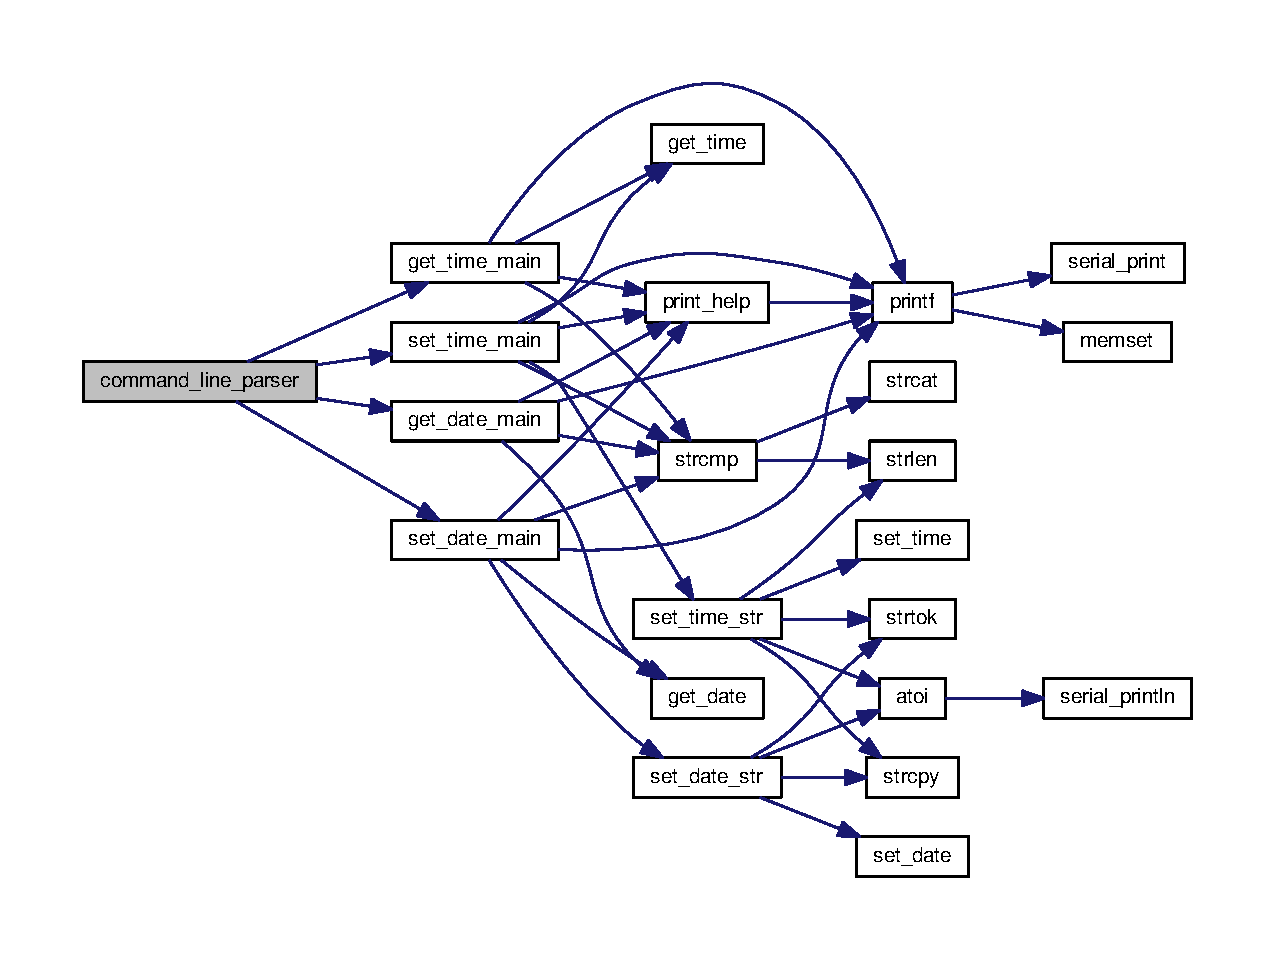
\includegraphics[width=350pt]{r1_8h_adb6b307c73bca25d17aa7683e14fea16_cgraph}
\end{center}
\end{figure}




Here is the caller graph for this function\+:\nopagebreak
\begin{figure}[H]
\begin{center}
\leavevmode
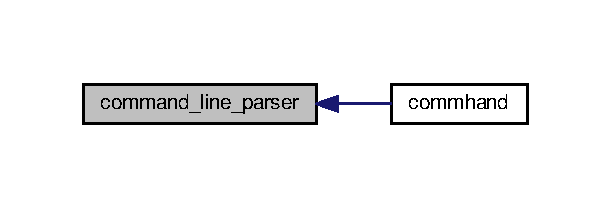
\includegraphics[width=293pt]{r1_8h_adb6b307c73bca25d17aa7683e14fea16_icgraph}
\end{center}
\end{figure}


\index{r1.\+h@{r1.\+h}!commhand@{commhand}}
\index{commhand@{commhand}!r1.\+h@{r1.\+h}}
\subsubsection[{\texorpdfstring{commhand()}{commhand()}}]{\setlength{\rightskip}{0pt plus 5cm}int commhand (
\begin{DoxyParamCaption}
{}
\end{DoxyParamCaption}
)}\hypertarget{r1_8h_a14d85617242501c323a203ee196d3efa}{}\label{r1_8h_a14d85617242501c323a203ee196d3efa}


Here is the call graph for this function\+:\nopagebreak
\begin{figure}[H]
\begin{center}
\leavevmode
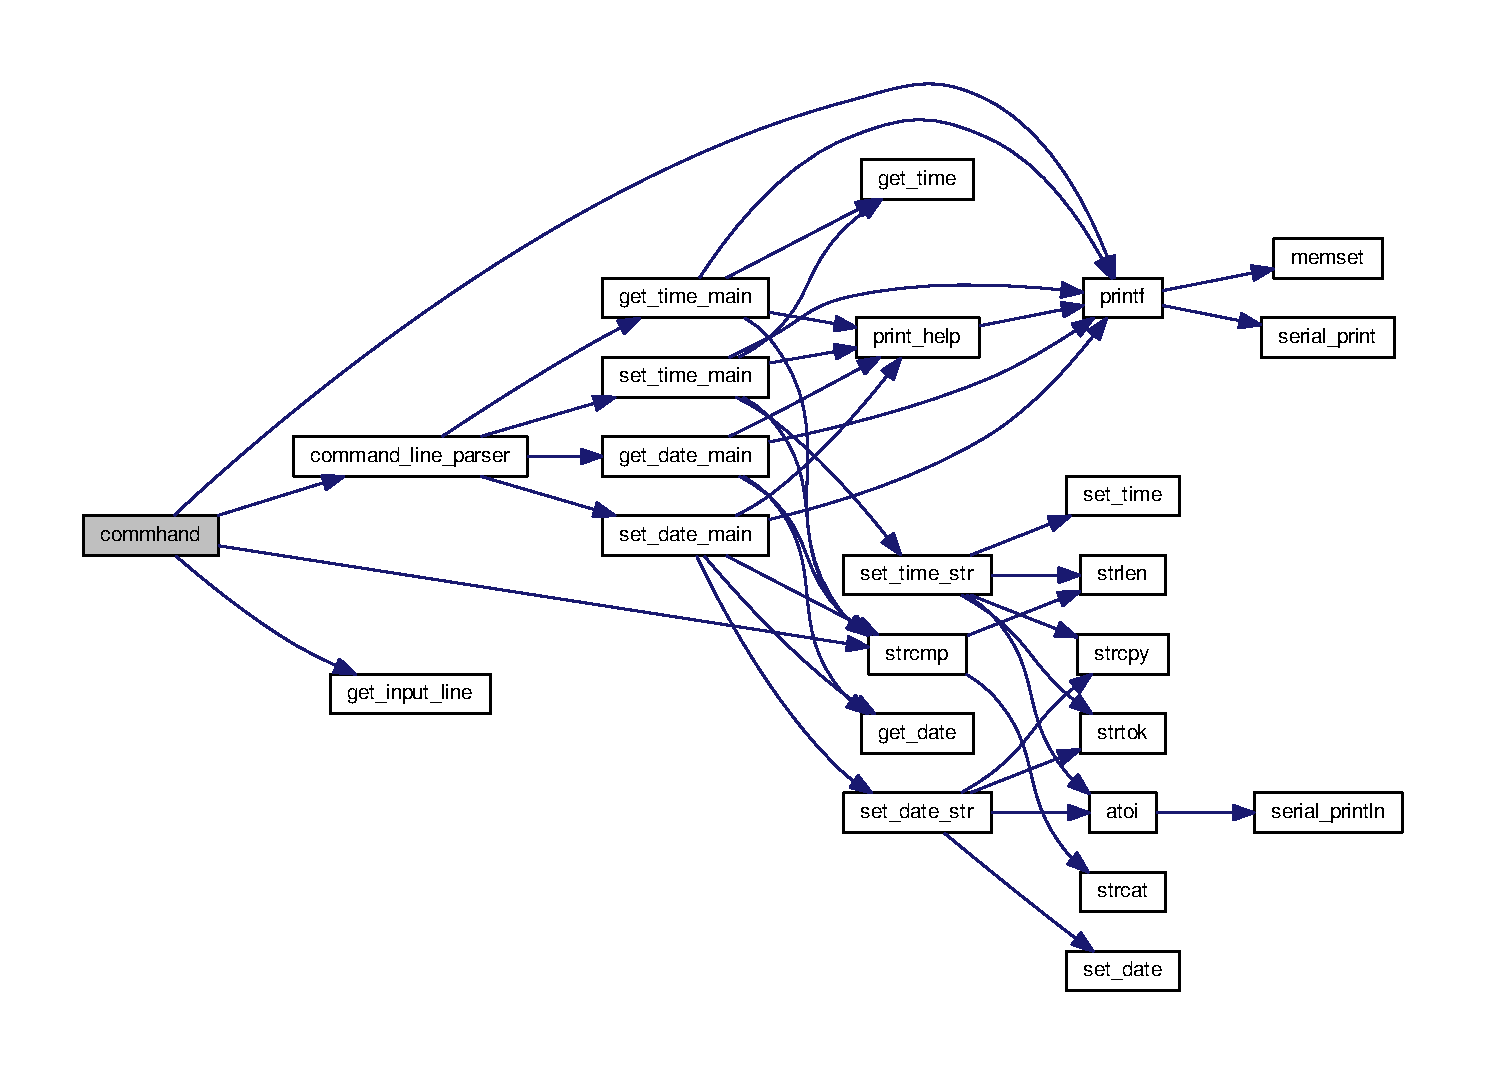
\includegraphics[width=350pt]{r1_8h_a14d85617242501c323a203ee196d3efa_cgraph}
\end{center}
\end{figure}


\index{r1.\+h@{r1.\+h}!print\+\_\+help@{print\+\_\+help}}
\index{print\+\_\+help@{print\+\_\+help}!r1.\+h@{r1.\+h}}
\subsubsection[{\texorpdfstring{print\+\_\+help(const int function\+\_\+index)}{print_help(const int function_index)}}]{\setlength{\rightskip}{0pt plus 5cm}void print\+\_\+help (
\begin{DoxyParamCaption}
\item[{const int}]{function\+\_\+index}
\end{DoxyParamCaption}
)}\hypertarget{r1_8h_ab5b36414d84437d45b388232a0dfa366}{}\label{r1_8h_ab5b36414d84437d45b388232a0dfa366}


Here is the call graph for this function\+:\nopagebreak
\begin{figure}[H]
\begin{center}
\leavevmode
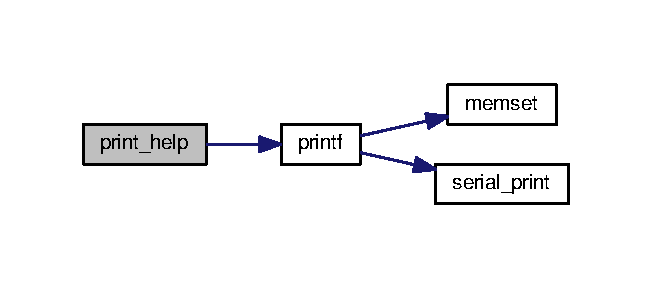
\includegraphics[width=313pt]{r1_8h_ab5b36414d84437d45b388232a0dfa366_cgraph}
\end{center}
\end{figure}




Here is the caller graph for this function\+:\nopagebreak
\begin{figure}[H]
\begin{center}
\leavevmode
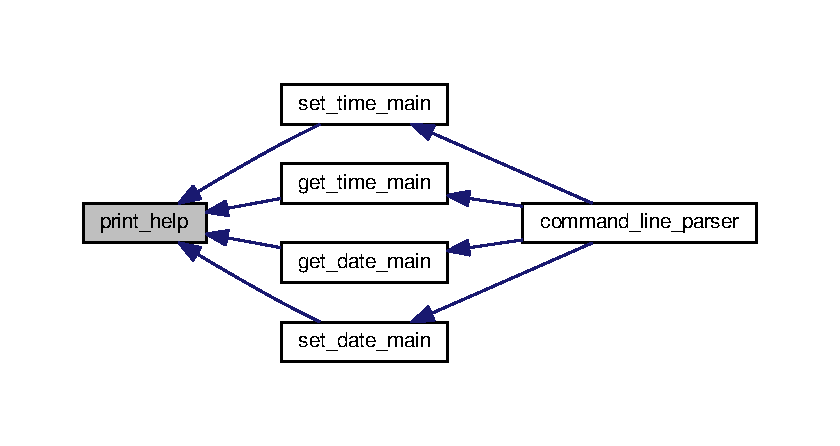
\includegraphics[width=350pt]{r1_8h_ab5b36414d84437d45b388232a0dfa366_icgraph}
\end{center}
\end{figure}



\hypertarget{sys__clock_8c}{}\section{modules/r1/sys\+\_\+clock.c File Reference}
\label{sys__clock_8c}\index{modules/r1/sys\+\_\+clock.\+c@{modules/r1/sys\+\_\+clock.\+c}}


The main file that manipulates and controls the system\textquotesingle{}s clock.  


{\ttfamily \#include \char`\"{}sys\+\_\+clock.\+h\char`\"{}}\\*
{\ttfamily \#include \char`\"{}r1.\+h\char`\"{}}\\*
{\ttfamily \#include $<$string.\+h$>$}\\*
{\ttfamily \#include $<$core/io.\+h$>$}\\*
\subsection*{Macros}
\begin{DoxyCompactItemize}
\item 
\#define {\bfseries R\+T\+C\+\_\+\+I\+N\+D\+E\+X\+\_\+\+S\+E\+C\+O\+ND}~0x00\hypertarget{sys__clock_8c_a4caca5127bfc14a5d2b8109573a7e650}{}\label{sys__clock_8c_a4caca5127bfc14a5d2b8109573a7e650}

\item 
\#define {\bfseries R\+T\+C\+\_\+\+I\+N\+D\+E\+X\+\_\+\+S\+E\+C\+O\+N\+D\+\_\+\+A\+L\+A\+RM}~0x01\hypertarget{sys__clock_8c_af180a80c181975cf0bf66868b689a72a}{}\label{sys__clock_8c_af180a80c181975cf0bf66868b689a72a}

\item 
\#define {\bfseries R\+T\+C\+\_\+\+I\+N\+D\+E\+X\+\_\+\+M\+I\+N\+U\+TE}~0x02\hypertarget{sys__clock_8c_a5f3ffb0e8042a3e0822291a9717a2b64}{}\label{sys__clock_8c_a5f3ffb0e8042a3e0822291a9717a2b64}

\item 
\#define {\bfseries R\+T\+C\+\_\+\+I\+N\+D\+E\+X\+\_\+\+M\+I\+N\+U\+T\+E\+\_\+\+A\+L\+A\+RM}~0x03\hypertarget{sys__clock_8c_ae3a9a93fc3485959b1aa57794ca17081}{}\label{sys__clock_8c_ae3a9a93fc3485959b1aa57794ca17081}

\item 
\#define {\bfseries R\+T\+C\+\_\+\+I\+N\+D\+E\+X\+\_\+\+H\+O\+UR}~0x04\hypertarget{sys__clock_8c_a14c92818941d0fc79172bf345c7d2da1}{}\label{sys__clock_8c_a14c92818941d0fc79172bf345c7d2da1}

\item 
\#define {\bfseries R\+T\+C\+\_\+\+I\+N\+D\+E\+X\+\_\+\+H\+O\+U\+R\+\_\+\+A\+L\+A\+RM}~0x05\hypertarget{sys__clock_8c_a698d910742dcdfcd400f416f682ffd0d}{}\label{sys__clock_8c_a698d910742dcdfcd400f416f682ffd0d}

\item 
\#define {\bfseries R\+T\+C\+\_\+\+I\+N\+D\+E\+X\+\_\+\+D\+A\+Y\+\_\+\+W\+E\+EK}~0x06\hypertarget{sys__clock_8c_ab605c9e34fb5f268a109de861f81fb64}{}\label{sys__clock_8c_ab605c9e34fb5f268a109de861f81fb64}

\item 
\#define {\bfseries R\+T\+C\+\_\+\+I\+N\+D\+E\+X\+\_\+\+D\+A\+Y\+\_\+\+M\+O\+N\+TH}~0x07\hypertarget{sys__clock_8c_a0bd4cec7882fb8084e54d5d137fb0b76}{}\label{sys__clock_8c_a0bd4cec7882fb8084e54d5d137fb0b76}

\item 
\#define {\bfseries R\+T\+C\+\_\+\+I\+N\+D\+E\+X\+\_\+\+M\+O\+N\+TH}~0x08\hypertarget{sys__clock_8c_af5ee5f7c5dbfcdf6df92fd558da7fc72}{}\label{sys__clock_8c_af5ee5f7c5dbfcdf6df92fd558da7fc72}

\item 
\#define {\bfseries R\+T\+C\+\_\+\+I\+N\+D\+E\+X\+\_\+\+Y\+E\+AR}~0x09\hypertarget{sys__clock_8c_a2f6fe8a8966f8fdabe2ddcf700786ce9}{}\label{sys__clock_8c_a2f6fe8a8966f8fdabe2ddcf700786ce9}

\end{DoxyCompactItemize}
\subsection*{Functions}
\begin{Indent}{\bf set\+\_\+time\+\_\+main.}\par
{\em Sets the time for the system.


\begin{DoxyParams}{Parameters}
{\em argc} & The number of tokens found. \\
\hline
{\em argv} & The array of tokens. \\
\hline
\end{DoxyParams}
\begin{DoxyReturn}{Returns}
0 
\end{DoxyReturn}
}\begin{DoxyCompactItemize}
\item 
int {\bfseries set\+\_\+time\+\_\+main} (int argc, char $\ast$$\ast$argv)\hypertarget{sys__clock_8c_a2afc871aeddaa550badc5e0c6bb65da5}{}\label{sys__clock_8c_a2afc871aeddaa550badc5e0c6bb65da5}

\end{DoxyCompactItemize}
\end{Indent}
\begin{Indent}{\bf get\+\_\+time\+\_\+main.}\par
{\em Retrieves system\textquotesingle{}s current time.


\begin{DoxyParams}{Parameters}
{\em argc} & The number of tokens found. \\
\hline
{\em argv} & The array of tokens. \\
\hline
\end{DoxyParams}
\begin{DoxyReturn}{Returns}
0 
\end{DoxyReturn}
}\begin{DoxyCompactItemize}
\item 
int {\bfseries get\+\_\+time\+\_\+main} (int argc, char $\ast$$\ast$argv)\hypertarget{sys__clock_8c_a323e417952cced55a3cf9acfe8691635}{}\label{sys__clock_8c_a323e417952cced55a3cf9acfe8691635}

\end{DoxyCompactItemize}
\end{Indent}
\begin{Indent}{\bf is\+\_\+digit}\par
{\em determines if a character represents a digit.


\begin{DoxyParams}{Parameters}
{\em ch} & The character\\
\hline
\end{DoxyParams}
\begin{DoxyReturn}{Returns}
1 if it is digit, otherwise returns 0. 
\end{DoxyReturn}
}\end{Indent}
\begin{Indent}{\bf set\+\_\+time\+\_\+str.}\par
{\em Sets the time for the system by string.


\begin{DoxyParams}{Parameters}
{\em time\+Str} & The string type of current Time. \\
\hline
\end{DoxyParams}
\begin{DoxyReturn}{Returns}
0 if there is no error, otherwise return a error code. 
\end{DoxyReturn}
}\begin{DoxyCompactItemize}
\item 
error\+\_\+t {\bfseries set\+\_\+time\+\_\+str} (const char $\ast$time\+Str)\hypertarget{sys__clock_8c_a2fa1ed5071047b72b357329da498b7aa}{}\label{sys__clock_8c_a2fa1ed5071047b72b357329da498b7aa}

\end{DoxyCompactItemize}
\end{Indent}
\begin{Indent}{\bf get\+\_\+time.}\par
{\em Retrieves system\textquotesingle{}s current time and date.


\begin{DoxyParams}{Parameters}
{\em date\+Time\+Values} & The value of current time and date \\
\hline
\end{DoxyParams}
\begin{DoxyReturn}{Returns}
V\+O\+ID 
\end{DoxyReturn}
}\begin{DoxyCompactItemize}
\item 
void {\bfseries get\+\_\+time} (date\+\_\+time $\ast$date\+Time\+Values)\hypertarget{sys__clock_8c_ac5f4cb4c73245c0bf8593116fa5580e9}{}\label{sys__clock_8c_ac5f4cb4c73245c0bf8593116fa5580e9}

\end{DoxyCompactItemize}
\end{Indent}
\begin{Indent}{\bf set\+\_\+time.}\par
{\em Sets the time for the system by date\+\_\+time struct.


\begin{DoxyParams}{Parameters}
{\em date\+Time\+Values} & The struct that holds the time values. \\
\hline
\end{DoxyParams}
\begin{DoxyReturn}{Returns}
0 if there is no error, otherwise return a error code. 
\end{DoxyReturn}
}\begin{DoxyCompactItemize}
\item 
error\+\_\+t {\bfseries set\+\_\+time} (const date\+\_\+time $\ast$date\+Time\+Values)\hypertarget{sys__clock_8c_a45d698fc822d2a31f93ee49057892800}{}\label{sys__clock_8c_a45d698fc822d2a31f93ee49057892800}

\end{DoxyCompactItemize}
\end{Indent}
\begin{Indent}{\bf get\+\_\+date.}\par
{\em Retrieves system\textquotesingle{}s current date.


\begin{DoxyParams}{Parameters}
{\em date\+Time\+Values} & The struct that holds the value of current date \\
\hline
\end{DoxyParams}
\begin{DoxyReturn}{Returns}
V\+O\+ID 
\end{DoxyReturn}
}\begin{DoxyCompactItemize}
\item 
void {\bfseries get\+\_\+date} (date\+\_\+time $\ast$date\+Time\+Values)\hypertarget{sys__clock_8c_acba98d47b98d09cf32f44e9383cad7ec}{}\label{sys__clock_8c_acba98d47b98d09cf32f44e9383cad7ec}

\end{DoxyCompactItemize}
\end{Indent}
\begin{Indent}{\bf \+: set\+\_\+date.}\par
{\em Sets the date of the system.


\begin{DoxyParams}{Parameters}
{\em date\+Time\+Values} & The struct that holds the value of date \\
\hline
\end{DoxyParams}
\begin{DoxyReturn}{Returns}
0 if there is no error, otherwise return a error code. 
\end{DoxyReturn}
}\begin{DoxyCompactItemize}
\item 
error\+\_\+t {\bfseries set\+\_\+date} (const date\+\_\+time $\ast$date\+Time\+Values)\hypertarget{sys__clock_8c_a5e0c140320ec0309fab102e2ad34d279}{}\label{sys__clock_8c_a5e0c140320ec0309fab102e2ad34d279}

\end{DoxyCompactItemize}
\end{Indent}
\begin{Indent}{\bf get\+\_\+date\+\_\+main.}\par
{\em Retrieves system\textquotesingle{}s current date.


\begin{DoxyParams}{Parameters}
{\em argc} & The number of tokens. \\
\hline
{\em argv} & The array of tokens. \\
\hline
\end{DoxyParams}
\begin{DoxyReturn}{Returns}
0 
\end{DoxyReturn}
}\begin{DoxyCompactItemize}
\item 
int {\bfseries get\+\_\+date\+\_\+main} (int argc, char $\ast$$\ast$argv)\hypertarget{sys__clock_8c_a1ef51abc1a538e8582ccfa61e356e8a9}{}\label{sys__clock_8c_a1ef51abc1a538e8582ccfa61e356e8a9}

\end{DoxyCompactItemize}
\end{Indent}
\begin{Indent}{\bf set\+\_\+date\+\_\+str.}\par
{\em Sets the date for the system by string.


\begin{DoxyParams}{Parameters}
{\em str} & The string type of current date. \\
\hline
\end{DoxyParams}
\begin{DoxyReturn}{Returns}
0 if there is no error, otherwise return a error code. 
\end{DoxyReturn}
}\begin{DoxyCompactItemize}
\item 
int {\bfseries set\+\_\+date\+\_\+str} (const char $\ast$str)\hypertarget{sys__clock_8c_ab80d04ed8d251aaea6a09fd01e68eb27}{}\label{sys__clock_8c_ab80d04ed8d251aaea6a09fd01e68eb27}

\end{DoxyCompactItemize}
\end{Indent}
\begin{Indent}{\bf set\+\_\+date\+\_\+main.}\par
{\em Sets system\textquotesingle{}s date.


\begin{DoxyParams}{Parameters}
{\em argc} & The number of tokens. \\
\hline
{\em argv} & The array of tokens. \\
\hline
\end{DoxyParams}
\begin{DoxyReturn}{Returns}
0 
\end{DoxyReturn}
}\begin{DoxyCompactItemize}
\item 
int {\bfseries set\+\_\+date\+\_\+main} (int argc, char $\ast$$\ast$argv)\hypertarget{sys__clock_8c_a626404928f9803307b300e6c60df3afb}{}\label{sys__clock_8c_a626404928f9803307b300e6c60df3afb}

\end{DoxyCompactItemize}
\end{Indent}


\subsection{Detailed Description}
The main file that manipulates and controls the system\textquotesingle{}s clock. 

\begin{DoxyAuthor}{Author}
Thunder Krakens 
\end{DoxyAuthor}
\begin{DoxyDate}{Date}
February 2nd, 2016 
\end{DoxyDate}
\begin{DoxyVersion}{Version}
R1 
\end{DoxyVersion}

\hypertarget{sys__clock_8h}{}\section{modules/r1/sys\+\_\+clock.h File Reference}
\label{sys__clock_8h}\index{modules/r1/sys\+\_\+clock.\+h@{modules/r1/sys\+\_\+clock.\+h}}


The main file that manipulates and controls the system\textquotesingle{}s clock.  


{\ttfamily \#include $<$system.\+h$>$}\\*
{\ttfamily \#include \char`\"{}../errno.\+h\char`\"{}}\\*
\subsection*{Functions}
\begin{Indent}{\bf set\+\_\+time\+\_\+main.}\par
{\em Sets the time for the system.


\begin{DoxyParams}{Parameters}
{\em argc} & The number of tokens found. \\
\hline
{\em argv} & The array of tokens. \\
\hline
\end{DoxyParams}
\begin{DoxyReturn}{Returns}
0 
\end{DoxyReturn}
}\begin{DoxyCompactItemize}
\item 
int {\bfseries set\+\_\+time\+\_\+main} (int argc, char $\ast$$\ast$argv)\hypertarget{sys__clock_8h_a2afc871aeddaa550badc5e0c6bb65da5}{}\label{sys__clock_8h_a2afc871aeddaa550badc5e0c6bb65da5}

\end{DoxyCompactItemize}
\end{Indent}
\begin{Indent}{\bf get\+\_\+time\+\_\+main.}\par
{\em Retrieves system\textquotesingle{}s current time.


\begin{DoxyParams}{Parameters}
{\em argc} & The number of tokens found. \\
\hline
{\em argv} & The array of tokens. \\
\hline
\end{DoxyParams}
\begin{DoxyReturn}{Returns}
0 
\end{DoxyReturn}
}\begin{DoxyCompactItemize}
\item 
int {\bfseries get\+\_\+time\+\_\+main} (int argc, char $\ast$$\ast$argv)\hypertarget{sys__clock_8h_a323e417952cced55a3cf9acfe8691635}{}\label{sys__clock_8h_a323e417952cced55a3cf9acfe8691635}

\end{DoxyCompactItemize}
\end{Indent}
\begin{Indent}{\bf set\+\_\+time\+\_\+str.}\par
{\em Sets the time for the system by string.


\begin{DoxyParams}{Parameters}
{\em time\+Str} & The string type of current Time. \\
\hline
\end{DoxyParams}
\begin{DoxyReturn}{Returns}
0 if there is no error, otherwise return a error code. 
\end{DoxyReturn}
}\begin{DoxyCompactItemize}
\item 
error\+\_\+t {\bfseries set\+\_\+time\+\_\+str} (const char $\ast$time\+Str)\hypertarget{sys__clock_8h_a2fa1ed5071047b72b357329da498b7aa}{}\label{sys__clock_8h_a2fa1ed5071047b72b357329da498b7aa}

\end{DoxyCompactItemize}
\end{Indent}
\begin{Indent}{\bf get\+\_\+time.}\par
{\em Retrieves system\textquotesingle{}s current time and date.


\begin{DoxyParams}{Parameters}
{\em date\+Time\+Values} & The value of current time and date \\
\hline
\end{DoxyParams}
\begin{DoxyReturn}{Returns}
V\+O\+ID 
\end{DoxyReturn}
}\begin{DoxyCompactItemize}
\item 
void {\bfseries get\+\_\+time} (date\+\_\+time $\ast$date\+Time\+Values)\hypertarget{sys__clock_8h_ac5f4cb4c73245c0bf8593116fa5580e9}{}\label{sys__clock_8h_ac5f4cb4c73245c0bf8593116fa5580e9}

\end{DoxyCompactItemize}
\end{Indent}
\begin{Indent}{\bf set\+\_\+time.}\par
{\em Sets the time for the system by date\+\_\+time struct.


\begin{DoxyParams}{Parameters}
{\em date\+Time\+Values} & The struct that holds the time values. \\
\hline
\end{DoxyParams}
\begin{DoxyReturn}{Returns}
0 if there is no error, otherwise return a error code. 
\end{DoxyReturn}
}\begin{DoxyCompactItemize}
\item 
error\+\_\+t {\bfseries set\+\_\+time} (const date\+\_\+time $\ast$date\+Time\+Values)\hypertarget{sys__clock_8h_a45d698fc822d2a31f93ee49057892800}{}\label{sys__clock_8h_a45d698fc822d2a31f93ee49057892800}

\end{DoxyCompactItemize}
\end{Indent}
\begin{Indent}{\bf set\+\_\+date\+\_\+main.}\par
{\em Sets system\textquotesingle{}s date.


\begin{DoxyParams}{Parameters}
{\em argc} & The number of tokens. \\
\hline
{\em argv} & The array of tokens. \\
\hline
\end{DoxyParams}
\begin{DoxyReturn}{Returns}
0 
\end{DoxyReturn}
}\begin{DoxyCompactItemize}
\item 
int {\bfseries set\+\_\+date\+\_\+main} (int argc, char $\ast$$\ast$argv)\hypertarget{sys__clock_8h_a626404928f9803307b300e6c60df3afb}{}\label{sys__clock_8h_a626404928f9803307b300e6c60df3afb}

\end{DoxyCompactItemize}
\end{Indent}
\begin{Indent}{\bf get\+\_\+date\+\_\+main.}\par
{\em Retrieves system\textquotesingle{}s current date.


\begin{DoxyParams}{Parameters}
{\em argc} & The number of tokens. \\
\hline
{\em argv} & The array of tokens. \\
\hline
\end{DoxyParams}
\begin{DoxyReturn}{Returns}
0 
\end{DoxyReturn}
}\begin{DoxyCompactItemize}
\item 
int {\bfseries get\+\_\+date\+\_\+main} (int argc, char $\ast$$\ast$argv)\hypertarget{sys__clock_8h_a1ef51abc1a538e8582ccfa61e356e8a9}{}\label{sys__clock_8h_a1ef51abc1a538e8582ccfa61e356e8a9}

\end{DoxyCompactItemize}
\end{Indent}
\begin{Indent}{\bf get\+\_\+date.}\par
{\em Retrieves system\textquotesingle{}s current date.


\begin{DoxyParams}{Parameters}
{\em date\+Time\+Values} & The struct that holds the value of current date \\
\hline
\end{DoxyParams}
\begin{DoxyReturn}{Returns}
V\+O\+ID 
\end{DoxyReturn}
}\begin{DoxyCompactItemize}
\item 
void {\bfseries get\+\_\+date} (date\+\_\+time $\ast$date\+Time\+Values)\hypertarget{sys__clock_8h_acba98d47b98d09cf32f44e9383cad7ec}{}\label{sys__clock_8h_acba98d47b98d09cf32f44e9383cad7ec}

\end{DoxyCompactItemize}
\end{Indent}
\begin{Indent}{\bf set\+\_\+date\+\_\+str.}\par
{\em Sets the date for the system by string.


\begin{DoxyParams}{Parameters}
{\em str} & The string type of current date. \\
\hline
\end{DoxyParams}
\begin{DoxyReturn}{Returns}
0 if there is no error, otherwise return a error code. 
\end{DoxyReturn}
}\begin{DoxyCompactItemize}
\item 
int {\bfseries set\+\_\+date\+\_\+str} (const char $\ast$str)\hypertarget{sys__clock_8h_ab80d04ed8d251aaea6a09fd01e68eb27}{}\label{sys__clock_8h_ab80d04ed8d251aaea6a09fd01e68eb27}

\end{DoxyCompactItemize}
\end{Indent}
\begin{Indent}{\bf \+: set\+\_\+date.}\par
{\em Sets the date of the system.


\begin{DoxyParams}{Parameters}
{\em date\+Time\+Values} & The struct that holds the value of date \\
\hline
\end{DoxyParams}
\begin{DoxyReturn}{Returns}
0 if there is no error, otherwise return a error code. 
\end{DoxyReturn}
}\begin{DoxyCompactItemize}
\item 
error\+\_\+t {\bfseries set\+\_\+date} (const date\+\_\+time $\ast$date\+Time\+Values)\hypertarget{sys__clock_8h_a5e0c140320ec0309fab102e2ad34d279}{}\label{sys__clock_8h_a5e0c140320ec0309fab102e2ad34d279}

\end{DoxyCompactItemize}
\end{Indent}


\subsection{Detailed Description}
The main file that manipulates and controls the system\textquotesingle{}s clock. 

\begin{DoxyAuthor}{Author}
Thunder Krakens 
\end{DoxyAuthor}
\begin{DoxyDate}{Date}
February 2nd, 2016 
\end{DoxyDate}
\begin{DoxyVersion}{Version}
R1 
\end{DoxyVersion}

\hypertarget{pcb_8c}{\section{modules/r2/pcb.c File Reference}
\label{pcb_8c}\index{modules/r2/pcb.\-c@{modules/r2/pcb.\-c}}
}


The Process Control Block.  


{\ttfamily \#include \char`\"{}pcb.\-h\char`\"{}}\\*
{\ttfamily \#include $<$string.\-h$>$}\\*
{\ttfamily \#include \char`\"{}../mpx\-\_\-supt.\-h\char`\"{}}\\*
Include dependency graph for pcb.\-c\-:\nopagebreak
\begin{figure}[H]
\begin{center}
\leavevmode
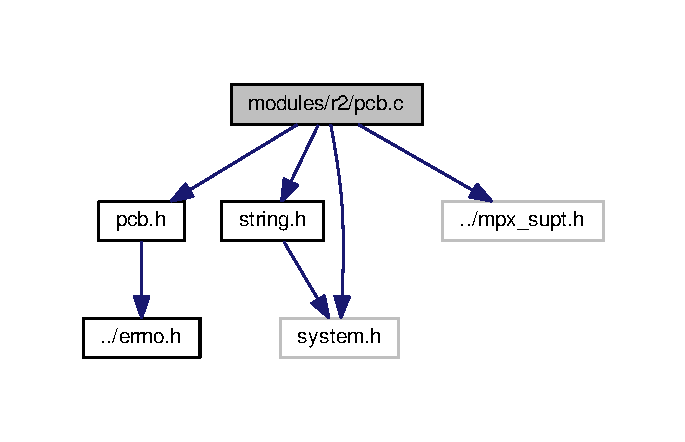
\includegraphics[width=329pt]{pcb_8c__incl}
\end{center}
\end{figure}
\subsection*{Data Structures}
\begin{DoxyCompactItemize}
\item 
struct \hyperlink{structpcb__struct}{pcb\-\_\-struct}
\begin{DoxyCompactList}\small\item\em Struct that will describe P\-C\-B Processes. \end{DoxyCompactList}\item 
struct \hyperlink{structpcb__queue}{pcb\-\_\-queue}
\begin{DoxyCompactList}\small\item\em Queue structure that will store P\-C\-Bs. \end{DoxyCompactList}\end{DoxyCompactItemize}
\subsection*{Enumerations}
\begin{DoxyCompactItemize}
\item 
enum \hyperlink{pcb_8c_a4e1a76273cf189daed25256e3ba34aef}{process\-\_\-state} 
\begin{DoxyCompactList}\small\item\em P\-C\-B process states/statuses. \end{DoxyCompactList}\item 
enum \hyperlink{pcb_8c_ac80b09976226d1f179d0911462a93034}{process\-\_\-suspended} 
\begin{DoxyCompactList}\small\item\em P\-C\-B process suspended or not suspended status. \end{DoxyCompactList}\end{DoxyCompactItemize}
\subsection*{Functions}
\begin{DoxyCompactItemize}
\item 
enum \hyperlink{pcb_8c_a4e1a76273cf189daed25256e3ba34aef}{process\-\_\-state} \hyperlink{pcb_8c_a8c731ad891b35b4876c5ce638d5c1b35}{\-\_\-\-\_\-attribute\-\_\-\-\_\-} ((packed))
\end{DoxyCompactItemize}
\begin{Indent}{\bf pcb\-\_\-init}\par
{\em Initiates the P\-C\-B queues}\begin{DoxyCompactItemize}
\item 
void \hyperlink{pcb_8c_a8d00fee50178510712d2ffeaeafae347}{pcb\-\_\-init} ()
\end{DoxyCompactItemize}
\end{Indent}
\begin{Indent}{\bf suspend\-\_\-pcb}\par
{\em Suspends the specific P\-C\-B.


\begin{DoxyParams}{Parameters}
{\em pcb\-\_\-ptr} & The pointer to the P\-C\-B\\
\hline
\end{DoxyParams}
\begin{DoxyReturn}{Returns}
The error code. Possible error code to be returned\-: E\-\_\-\-N\-O\-E\-R\-R\-O\-R No error. E\-\_\-\-N\-U\-L\-L\-\_\-\-P\-T\-R Null pointer error. 
\end{DoxyReturn}
}\begin{DoxyCompactItemize}
\item 
\hyperlink{errno_8h_aafbeb34410283829794b35fedafeb369}{error\-\_\-t} \hyperlink{pcb_8c_acb4a05dff84e0ad1777c1991f95be1e0}{suspend\-\_\-pcb} (struct \hyperlink{structpcb__struct}{pcb\-\_\-struct} $\ast$pcb\-\_\-ptr)
\end{DoxyCompactItemize}
\end{Indent}
\begin{Indent}{\bf resume\-\_\-pcb}\par
{\em Resumes the specific P\-C\-B.


\begin{DoxyParams}{Parameters}
{\em pcb\-\_\-ptr} & The pointer to the P\-C\-B\\
\hline
\end{DoxyParams}
\begin{DoxyReturn}{Returns}
The error code. Possible error code to be returned\-: E\-\_\-\-N\-O\-E\-R\-R\-O\-R No error. E\-\_\-\-N\-U\-L\-L\-\_\-\-P\-T\-R Null pointer error. 
\end{DoxyReturn}
}\begin{DoxyCompactItemize}
\item 
\hyperlink{errno_8h_aafbeb34410283829794b35fedafeb369}{error\-\_\-t} \hyperlink{pcb_8c_a24a874ae323c9ef0583c2f179b44fe74}{resume\-\_\-pcb} (struct \hyperlink{structpcb__struct}{pcb\-\_\-struct} $\ast$pcb\-\_\-ptr)
\end{DoxyCompactItemize}
\end{Indent}
\begin{Indent}{\bf allocate\-\_\-pcb}\par
{\em allocate a space for the P\-C\-B structure.

\begin{DoxyReturn}{Returns}
The pointer that point to the P\-C\-B structure. 
\end{DoxyReturn}
}\begin{DoxyCompactItemize}
\item 
struct \hyperlink{structpcb__struct}{pcb\-\_\-struct} $\ast$ \hyperlink{pcb_8c_a8fd9eebd60b5c6838b055b6dab7065e1}{allocate\-\_\-pcb} ()
\end{DoxyCompactItemize}
\end{Indent}
\begin{Indent}{\bf setup\-\_\-pcb}\par
{\em allocate a space for the P\-C\-B structure, setup the properties of the P\-C\-B.

N\-O\-T\-E\-: p\-Name must less than 10 character, p\-Class should be either \char`\"{}application\char`\"{} or \char`\"{}system\char`\"{} , and p\-Priority must within the range of \mbox{[}0, 9\mbox{]}.


\begin{DoxyParams}{Parameters}
{\em p\-Name} & Process Name (length $<$ 10). \\
\hline
{\em p\-Class} & Process class (system or application). \\
\hline
{\em p\-Priority} & Process priority (0 $\sim$ 9).\\
\hline
\end{DoxyParams}
\begin{DoxyReturn}{Returns}
N\-U\-L\-L if error occured, otherwise, the pointer that point to the P\-C\-B structure. 
\end{DoxyReturn}
}\begin{DoxyCompactItemize}
\item 
struct \hyperlink{structpcb__struct}{pcb\-\_\-struct} $\ast$ \hyperlink{pcb_8c_aa8ef2e50138f1b01310c83d261c2efa9}{setup\-\_\-pcb} (const char $\ast$p\-Name, const enum \hyperlink{pcb_8h_aefe309d62b55b4d0be96f1a97fcbbadd}{process\-\_\-class} p\-Class, const unsigned char p\-Priority)
\end{DoxyCompactItemize}
\end{Indent}
\begin{Indent}{\bf free\-\_\-pcb}\par
{\em Frees all memory associated with given P\-C\-B, including the P\-C\-B itself, the stack, etc, with sys\-\_\-free\-\_\-mem()


\begin{DoxyParams}{Parameters}
{\em pcb\-\_\-ptr} & The pointer to the P\-C\-B\\
\hline
\end{DoxyParams}
\begin{DoxyReturn}{Returns}
The error code. Possible error code to be returned\-: E\-\_\-\-N\-O\-E\-R\-R\-O\-R No error. E\-\_\-\-I\-N\-V\-P\-A\-R\-A The P\-C\-B probably had not been removed from queue before free it. E\-\_\-\-F\-R\-E\-E\-M\-E\-M The memory space cannot be actually free, since the student\-\_\-free had not been implemented yet. 
\end{DoxyReturn}
}\begin{DoxyCompactItemize}
\item 
\hyperlink{errno_8h_aafbeb34410283829794b35fedafeb369}{error\-\_\-t} \hyperlink{pcb_8c_a31e603695448c5bd7bccacce5988eaf2}{free\-\_\-pcb} (struct \hyperlink{structpcb__struct}{pcb\-\_\-struct} $\ast$pcb\-\_\-ptr)
\end{DoxyCompactItemize}
\end{Indent}
\begin{Indent}{\bf find\-\_\-pcb}\par
{\em Will search all queues for a process named p\-Name


\begin{DoxyParams}{Parameters}
{\em p\-Name} & The char pointer to the desired searched name\\
\hline
\end{DoxyParams}
\begin{DoxyReturn}{Returns}
P\-C\-B pointer if found, N\-U\-L\-L if P\-C\-B is not found 
\end{DoxyReturn}
}\begin{DoxyCompactItemize}
\item 
struct \hyperlink{structpcb__struct}{pcb\-\_\-struct} $\ast$ \hyperlink{pcb_8c_acfbb91c24a4b3cdc22d9a27df468013d}{find\-\_\-pcb} (const char $\ast$p\-Name)
\end{DoxyCompactItemize}
\end{Indent}
\begin{Indent}{\bf insert\-\_\-pcb}\par
{\em Inserts P\-C\-B into the appropriate queue.


\begin{DoxyParams}{Parameters}
{\em pcb\-\_\-ptr} & The pointer to the P\-C\-B\\
\hline
\end{DoxyParams}
\begin{DoxyReturn}{Returns}
The error code. Possible error code to be returned\-: E\-\_\-\-N\-O\-E\-R\-R\-O\-R No error. E\-\_\-\-N\-U\-L\-L\-\_\-\-P\-T\-R Null pointer error. E\-\_\-\-I\-N\-V\-P\-A\-R\-A The given P\-C\-B has running status or abnormal data members. 
\end{DoxyReturn}
}\begin{DoxyCompactItemize}
\item 
\hyperlink{errno_8h_aafbeb34410283829794b35fedafeb369}{error\-\_\-t} \hyperlink{pcb_8c_ae8f8cca202f2232d4396a48db14b7d35}{insert\-\_\-pcb} (struct \hyperlink{structpcb__struct}{pcb\-\_\-struct} $\ast$pcb\-\_\-ptr)
\end{DoxyCompactItemize}
\end{Indent}
\begin{Indent}{\bf remove\-\_\-pcb}\par
{\em Removes P\-C\-B from the queue it is currently in.


\begin{DoxyParams}{Parameters}
{\em pcb\-\_\-ptr} & The pointer to the P\-C\-B\\
\hline
\end{DoxyParams}
\begin{DoxyReturn}{Returns}
The error code. Possible error code to be returned\-: E\-\_\-\-N\-O\-E\-R\-R\-O\-R No error. E\-\_\-\-N\-U\-L\-L\-\_\-\-P\-T\-R Null pointer error. E\-\_\-\-I\-N\-V\-P\-A\-R\-A The given P\-C\-B has abnormal data members. 
\end{DoxyReturn}
}\begin{DoxyCompactItemize}
\item 
\hyperlink{errno_8h_aafbeb34410283829794b35fedafeb369}{error\-\_\-t} \hyperlink{pcb_8c_a52620da5c66ed459beea65538169547a}{remove\-\_\-pcb} (struct \hyperlink{structpcb__struct}{pcb\-\_\-struct} $\ast$pcb\-\_\-ptr)
\end{DoxyCompactItemize}
\end{Indent}
\begin{Indent}{\bf show\-\_\-pcb}\par
{\em Displays the name, class, state, suspend status, and priority of a P\-C\-B.


\begin{DoxyParams}{Parameters}
{\em p\-Name} & The P\-C\-B pointer. \\
\hline
\end{DoxyParams}
\begin{DoxyReturn}{Returns}
The error code. Possible error code to be returned\-: E\-\_\-\-N\-O\-E\-R\-R\-O\-R No error. E\-\_\-\-N\-U\-L\-L\-\_\-\-P\-T\-R Null pointer error. 
\end{DoxyReturn}
}\begin{DoxyCompactItemize}
\item 
\hyperlink{errno_8h_aafbeb34410283829794b35fedafeb369}{error\-\_\-t} \hyperlink{pcb_8c_af08c093fa9ecf34738d5e295520a032a}{show\-\_\-pcb} (struct \hyperlink{structpcb__struct}{pcb\-\_\-struct} $\ast$pcb\-\_\-ptr)
\end{DoxyCompactItemize}
\end{Indent}
\begin{Indent}{\bf show\-\_\-blocked\-\_\-processes}\par
{\em displays all blocked processes and their attributes

\begin{DoxyReturn}{Returns}
V\-O\-I\-D. 
\end{DoxyReturn}
}\begin{DoxyCompactItemize}
\item 
void \hyperlink{pcb_8c_a918cbc9698ab932896ec81c482fee9f1}{show\-\_\-blocked\-\_\-processes} ()
\end{DoxyCompactItemize}
\end{Indent}
\begin{Indent}{\bf show\-\_\-ready\-\_\-processes}\par
{\em Displays all of the ready processes and their attributes.

\begin{DoxyReturn}{Returns}
V\-O\-I\-D. 
\end{DoxyReturn}
}\begin{DoxyCompactItemize}
\item 
void \hyperlink{pcb_8c_a542627a44f5cbaf08ceaab05a419acee}{show\-\_\-ready\-\_\-processes} ()
\end{DoxyCompactItemize}
\end{Indent}
\begin{Indent}{\bf show\-\_\-all\-\_\-processes}\par
{\em Displays all of the processes and their attributes.

\begin{DoxyReturn}{Returns}
V\-O\-I\-D. 
\end{DoxyReturn}
}\begin{DoxyCompactItemize}
\item 
void \hyperlink{pcb_8c_a094b4bf39d7297266e9b1336a233841e}{show\-\_\-all\-\_\-processes} ()
\end{DoxyCompactItemize}
\end{Indent}
\begin{Indent}{\bf block\-\_\-pcb}\par
{\em puts the given pcb into the blocked state and places it into the correct queue


\begin{DoxyParams}{Parameters}
{\em pcb\-\_\-ptr} & The pointer to the P\-C\-B\\
\hline
\end{DoxyParams}
\begin{DoxyReturn}{Returns}
The error code. Possible error code to be returned\-: E\-\_\-\-N\-O\-E\-R\-R\-O\-R No error. E\-\_\-\-N\-U\-L\-L\-\_\-\-P\-T\-R Null pointer error. E\-\_\-\-I\-N\-V\-P\-A\-R\-A The given P\-C\-B has abnormal data members (By \char`\"{}remove\-\_\-pcb\char`\"{} or \char`\"{}insert\-\_\-pcb\char`\"{}). 
\end{DoxyReturn}
}\begin{DoxyCompactItemize}
\item 
\hyperlink{errno_8h_aafbeb34410283829794b35fedafeb369}{error\-\_\-t} \hyperlink{pcb_8c_aa5aad077eb0c15c0c76fc4522b11a410}{block\-\_\-pcb} (struct \hyperlink{structpcb__struct}{pcb\-\_\-struct} $\ast$pcb\-\_\-ptr)
\end{DoxyCompactItemize}
\end{Indent}
\begin{Indent}{\bf unblock\-\_\-pcb}\par
{\em puts the given pcb into the unblocked state and places it into the correct queue


\begin{DoxyParams}{Parameters}
{\em pcb\-\_\-ptr} & The pointer to the P\-C\-B\\
\hline
\end{DoxyParams}
\begin{DoxyReturn}{Returns}
The error code. Possible error code to be returned\-: E\-\_\-\-N\-O\-E\-R\-R\-O\-R No error. E\-\_\-\-N\-U\-L\-L\-\_\-\-P\-T\-R Null pointer error. E\-\_\-\-I\-N\-V\-P\-A\-R\-A The given P\-C\-B has abnormal data members (By \char`\"{}remove\-\_\-pcb\char`\"{} or \char`\"{}insert\-\_\-pcb\char`\"{}). 
\end{DoxyReturn}
}\begin{DoxyCompactItemize}
\item 
\hyperlink{errno_8h_aafbeb34410283829794b35fedafeb369}{error\-\_\-t} \hyperlink{pcb_8c_a0526b69c22b1961dad32f21f9b380f4b}{unblock\-\_\-pcb} (struct \hyperlink{structpcb__struct}{pcb\-\_\-struct} $\ast$pcb\-\_\-ptr)
\end{DoxyCompactItemize}
\end{Indent}
\begin{Indent}{\bf set\-\_\-pcb\-\_\-priority}\par
{\em Sets the priority of the selected P\-C\-B


\begin{DoxyParams}{Parameters}
{\em pcb\-\_\-ptr} & The P\-C\-B pointer. \\
\hline
{\em p\-Priorty} & The assigned priorirty \\
\hline
\end{DoxyParams}
\begin{DoxyReturn}{Returns}
The error code. Possible error code to be returned\-: E\-\_\-\-N\-O\-E\-R\-R\-O\-R No error. E\-\_\-\-N\-U\-L\-L\-\_\-\-P\-T\-R Null pointer error. E\-\_\-\-I\-N\-V\-P\-A\-R\-A The p\-Priority is out of range. Or, the given P\-C\-B has abnormal data members (By \char`\"{}remove\-\_\-pcb\char`\"{} or \char`\"{}insert\-\_\-pcb\char`\"{}). 
\end{DoxyReturn}
}\begin{DoxyCompactItemize}
\item 
\hyperlink{errno_8h_aafbeb34410283829794b35fedafeb369}{error\-\_\-t} \hyperlink{pcb_8c_a863d9b3d5113d72ebc7b64e01937fc97}{set\-\_\-pcb\-\_\-priority} (struct \hyperlink{structpcb__struct}{pcb\-\_\-struct} $\ast$pcb\-\_\-ptr, const unsigned char p\-Priority)
\end{DoxyCompactItemize}
\end{Indent}
\subsection*{Variables}
\begin{DoxyCompactItemize}
\item 
\hyperlink{pcb_8c_a1a015fe02c9cea18a5cf62656e257c97}{running}
\begin{DoxyCompactList}\small\item\em P\-C\-B in the running state. \end{DoxyCompactList}\item 
\hyperlink{pcb_8c_ab0db378e6ced1decdb42263d4cb2789a}{ready}
\begin{DoxyCompactList}\small\item\em P\-C\-B in the ready state. \end{DoxyCompactList}\item 
\hyperlink{pcb_8c_a1faaaae288fc8ca4ed1751049aa2f84f}{blocked}
\begin{DoxyCompactList}\small\item\em $<$ P\-C\-B in the blocked state. \end{DoxyCompactList}\item 
\hyperlink{pcb_8c_a1a24fc2eb8c1af6d06ac15bcec47f088}{true}
\begin{DoxyCompactList}\small\item\em P\-C\-B process is suspended. \end{DoxyCompactList}\item 
\hyperlink{pcb_8c_ae6c865df784842196d411c1466b01686}{false}
\begin{DoxyCompactList}\small\item\em $<$ P\-C\-B process is not suspended. \end{DoxyCompactList}\item 
struct \hyperlink{structpcb__struct}{pcb\-\_\-struct} \hyperlink{pcb_8c_a5e5a16f32884089aeed6b337440cf588}{\-\_\-\-\_\-attribute\-\_\-\-\_\-}
\end{DoxyCompactItemize}


\subsection{Detailed Description}
The Process Control Block. \begin{DoxyAuthor}{Author}
Thunder Krakens 
\end{DoxyAuthor}
\begin{DoxyDate}{Date}
February 7th, 2016 
\end{DoxyDate}
\begin{DoxyVersion}{Version}
R2 
\end{DoxyVersion}


\subsection{Enumeration Type Documentation}
\hypertarget{pcb_8c_a4e1a76273cf189daed25256e3ba34aef}{\index{pcb.\-c@{pcb.\-c}!process\-\_\-state@{process\-\_\-state}}
\index{process\-\_\-state@{process\-\_\-state}!pcb.c@{pcb.\-c}}
\subsubsection[{process\-\_\-state}]{\setlength{\rightskip}{0pt plus 5cm}enum {\bf process\-\_\-state}}}\label{pcb_8c_a4e1a76273cf189daed25256e3ba34aef}


P\-C\-B process states/statuses. 

\hypertarget{pcb_8c_ac80b09976226d1f179d0911462a93034}{\index{pcb.\-c@{pcb.\-c}!process\-\_\-suspended@{process\-\_\-suspended}}
\index{process\-\_\-suspended@{process\-\_\-suspended}!pcb.c@{pcb.\-c}}
\subsubsection[{process\-\_\-suspended}]{\setlength{\rightskip}{0pt plus 5cm}enum {\bf process\-\_\-suspended}}}\label{pcb_8c_ac80b09976226d1f179d0911462a93034}


P\-C\-B process suspended or not suspended status. 



\subsection{Function Documentation}
\hypertarget{pcb_8c_a8c731ad891b35b4876c5ce638d5c1b35}{\index{pcb.\-c@{pcb.\-c}!\-\_\-\-\_\-attribute\-\_\-\-\_\-@{\-\_\-\-\_\-attribute\-\_\-\-\_\-}}
\index{\-\_\-\-\_\-attribute\-\_\-\-\_\-@{\-\_\-\-\_\-attribute\-\_\-\-\_\-}!pcb.c@{pcb.\-c}}
\subsubsection[{\-\_\-\-\_\-attribute\-\_\-\-\_\-}]{\setlength{\rightskip}{0pt plus 5cm}enum {\bf process\-\_\-state} \-\_\-\-\_\-attribute\-\_\-\-\_\- (
\begin{DoxyParamCaption}
\item[{(packed)}]{}
\end{DoxyParamCaption}
)}}\label{pcb_8c_a8c731ad891b35b4876c5ce638d5c1b35}
\hypertarget{pcb_8c_a8fd9eebd60b5c6838b055b6dab7065e1}{\index{pcb.\-c@{pcb.\-c}!allocate\-\_\-pcb@{allocate\-\_\-pcb}}
\index{allocate\-\_\-pcb@{allocate\-\_\-pcb}!pcb.c@{pcb.\-c}}
\subsubsection[{allocate\-\_\-pcb}]{\setlength{\rightskip}{0pt plus 5cm}struct {\bf pcb\-\_\-struct}$\ast$ allocate\-\_\-pcb (
\begin{DoxyParamCaption}
{}
\end{DoxyParamCaption}
)}}\label{pcb_8c_a8fd9eebd60b5c6838b055b6dab7065e1}


Here is the caller graph for this function\-:\nopagebreak
\begin{figure}[H]
\begin{center}
\leavevmode
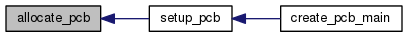
\includegraphics[width=350pt]{pcb_8c_a8fd9eebd60b5c6838b055b6dab7065e1_icgraph}
\end{center}
\end{figure}


\hypertarget{pcb_8c_aa5aad077eb0c15c0c76fc4522b11a410}{\index{pcb.\-c@{pcb.\-c}!block\-\_\-pcb@{block\-\_\-pcb}}
\index{block\-\_\-pcb@{block\-\_\-pcb}!pcb.c@{pcb.\-c}}
\subsubsection[{block\-\_\-pcb}]{\setlength{\rightskip}{0pt plus 5cm}{\bf error\-\_\-t} block\-\_\-pcb (
\begin{DoxyParamCaption}
\item[{struct {\bf pcb\-\_\-struct} $\ast$}]{pcb\-\_\-ptr}
\end{DoxyParamCaption}
)}}\label{pcb_8c_aa5aad077eb0c15c0c76fc4522b11a410}


Here is the call graph for this function\-:\nopagebreak
\begin{figure}[H]
\begin{center}
\leavevmode
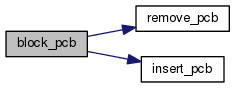
\includegraphics[width=248pt]{pcb_8c_aa5aad077eb0c15c0c76fc4522b11a410_cgraph}
\end{center}
\end{figure}




Here is the caller graph for this function\-:\nopagebreak
\begin{figure}[H]
\begin{center}
\leavevmode
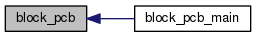
\includegraphics[width=266pt]{pcb_8c_aa5aad077eb0c15c0c76fc4522b11a410_icgraph}
\end{center}
\end{figure}


\hypertarget{pcb_8c_acfbb91c24a4b3cdc22d9a27df468013d}{\index{pcb.\-c@{pcb.\-c}!find\-\_\-pcb@{find\-\_\-pcb}}
\index{find\-\_\-pcb@{find\-\_\-pcb}!pcb.c@{pcb.\-c}}
\subsubsection[{find\-\_\-pcb}]{\setlength{\rightskip}{0pt plus 5cm}struct {\bf pcb\-\_\-struct}$\ast$ find\-\_\-pcb (
\begin{DoxyParamCaption}
\item[{const char $\ast$}]{p\-Name}
\end{DoxyParamCaption}
)}}\label{pcb_8c_acfbb91c24a4b3cdc22d9a27df468013d}


Here is the call graph for this function\-:\nopagebreak
\begin{figure}[H]
\begin{center}
\leavevmode
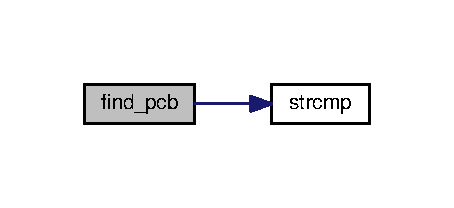
\includegraphics[width=218pt]{pcb_8c_acfbb91c24a4b3cdc22d9a27df468013d_cgraph}
\end{center}
\end{figure}




Here is the caller graph for this function\-:\nopagebreak
\begin{figure}[H]
\begin{center}
\leavevmode
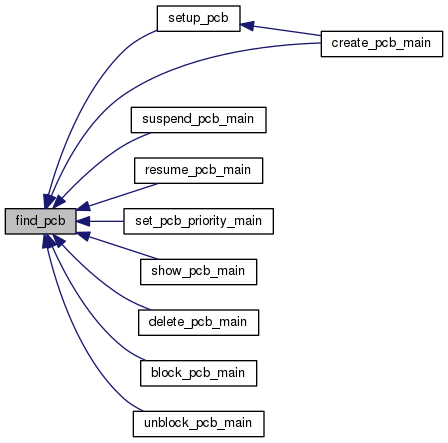
\includegraphics[width=350pt]{pcb_8c_acfbb91c24a4b3cdc22d9a27df468013d_icgraph}
\end{center}
\end{figure}


\hypertarget{pcb_8c_a31e603695448c5bd7bccacce5988eaf2}{\index{pcb.\-c@{pcb.\-c}!free\-\_\-pcb@{free\-\_\-pcb}}
\index{free\-\_\-pcb@{free\-\_\-pcb}!pcb.c@{pcb.\-c}}
\subsubsection[{free\-\_\-pcb}]{\setlength{\rightskip}{0pt plus 5cm}{\bf error\-\_\-t} free\-\_\-pcb (
\begin{DoxyParamCaption}
\item[{struct {\bf pcb\-\_\-struct} $\ast$}]{pcb\-\_\-ptr}
\end{DoxyParamCaption}
)}}\label{pcb_8c_a31e603695448c5bd7bccacce5988eaf2}


Here is the caller graph for this function\-:\nopagebreak
\begin{figure}[H]
\begin{center}
\leavevmode
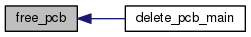
\includegraphics[width=260pt]{pcb_8c_a31e603695448c5bd7bccacce5988eaf2_icgraph}
\end{center}
\end{figure}


\hypertarget{pcb_8c_ae8f8cca202f2232d4396a48db14b7d35}{\index{pcb.\-c@{pcb.\-c}!insert\-\_\-pcb@{insert\-\_\-pcb}}
\index{insert\-\_\-pcb@{insert\-\_\-pcb}!pcb.c@{pcb.\-c}}
\subsubsection[{insert\-\_\-pcb}]{\setlength{\rightskip}{0pt plus 5cm}{\bf error\-\_\-t} insert\-\_\-pcb (
\begin{DoxyParamCaption}
\item[{struct {\bf pcb\-\_\-struct} $\ast$}]{pcb\-\_\-ptr}
\end{DoxyParamCaption}
)}}\label{pcb_8c_ae8f8cca202f2232d4396a48db14b7d35}


Here is the caller graph for this function\-:\nopagebreak
\begin{figure}[H]
\begin{center}
\leavevmode
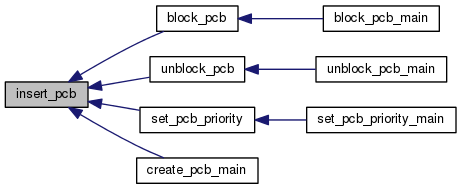
\includegraphics[width=350pt]{pcb_8c_ae8f8cca202f2232d4396a48db14b7d35_icgraph}
\end{center}
\end{figure}


\hypertarget{pcb_8c_a8d00fee50178510712d2ffeaeafae347}{\index{pcb.\-c@{pcb.\-c}!pcb\-\_\-init@{pcb\-\_\-init}}
\index{pcb\-\_\-init@{pcb\-\_\-init}!pcb.c@{pcb.\-c}}
\subsubsection[{pcb\-\_\-init}]{\setlength{\rightskip}{0pt plus 5cm}void pcb\-\_\-init (
\begin{DoxyParamCaption}
{}
\end{DoxyParamCaption}
)}}\label{pcb_8c_a8d00fee50178510712d2ffeaeafae347}
\hypertarget{pcb_8c_a52620da5c66ed459beea65538169547a}{\index{pcb.\-c@{pcb.\-c}!remove\-\_\-pcb@{remove\-\_\-pcb}}
\index{remove\-\_\-pcb@{remove\-\_\-pcb}!pcb.c@{pcb.\-c}}
\subsubsection[{remove\-\_\-pcb}]{\setlength{\rightskip}{0pt plus 5cm}{\bf error\-\_\-t} remove\-\_\-pcb (
\begin{DoxyParamCaption}
\item[{struct {\bf pcb\-\_\-struct} $\ast$}]{pcb\-\_\-ptr}
\end{DoxyParamCaption}
)}}\label{pcb_8c_a52620da5c66ed459beea65538169547a}


Here is the caller graph for this function\-:\nopagebreak
\begin{figure}[H]
\begin{center}
\leavevmode
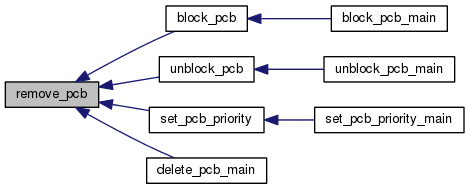
\includegraphics[width=350pt]{pcb_8c_a52620da5c66ed459beea65538169547a_icgraph}
\end{center}
\end{figure}


\hypertarget{pcb_8c_a24a874ae323c9ef0583c2f179b44fe74}{\index{pcb.\-c@{pcb.\-c}!resume\-\_\-pcb@{resume\-\_\-pcb}}
\index{resume\-\_\-pcb@{resume\-\_\-pcb}!pcb.c@{pcb.\-c}}
\subsubsection[{resume\-\_\-pcb}]{\setlength{\rightskip}{0pt plus 5cm}{\bf error\-\_\-t} resume\-\_\-pcb (
\begin{DoxyParamCaption}
\item[{struct {\bf pcb\-\_\-struct} $\ast$}]{pcb\-\_\-ptr}
\end{DoxyParamCaption}
)}}\label{pcb_8c_a24a874ae323c9ef0583c2f179b44fe74}


Here is the caller graph for this function\-:\nopagebreak
\begin{figure}[H]
\begin{center}
\leavevmode
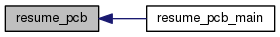
\includegraphics[width=282pt]{pcb_8c_a24a874ae323c9ef0583c2f179b44fe74_icgraph}
\end{center}
\end{figure}


\hypertarget{pcb_8c_a863d9b3d5113d72ebc7b64e01937fc97}{\index{pcb.\-c@{pcb.\-c}!set\-\_\-pcb\-\_\-priority@{set\-\_\-pcb\-\_\-priority}}
\index{set\-\_\-pcb\-\_\-priority@{set\-\_\-pcb\-\_\-priority}!pcb.c@{pcb.\-c}}
\subsubsection[{set\-\_\-pcb\-\_\-priority}]{\setlength{\rightskip}{0pt plus 5cm}{\bf error\-\_\-t} set\-\_\-pcb\-\_\-priority (
\begin{DoxyParamCaption}
\item[{struct {\bf pcb\-\_\-struct} $\ast$}]{pcb\-\_\-ptr, }
\item[{const unsigned char}]{p\-Priority}
\end{DoxyParamCaption}
)}}\label{pcb_8c_a863d9b3d5113d72ebc7b64e01937fc97}


Here is the call graph for this function\-:\nopagebreak
\begin{figure}[H]
\begin{center}
\leavevmode
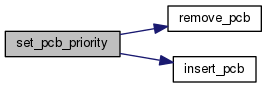
\includegraphics[width=272pt]{pcb_8c_a863d9b3d5113d72ebc7b64e01937fc97_cgraph}
\end{center}
\end{figure}




Here is the caller graph for this function\-:\nopagebreak
\begin{figure}[H]
\begin{center}
\leavevmode
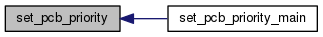
\includegraphics[width=314pt]{pcb_8c_a863d9b3d5113d72ebc7b64e01937fc97_icgraph}
\end{center}
\end{figure}


\hypertarget{pcb_8c_aa8ef2e50138f1b01310c83d261c2efa9}{\index{pcb.\-c@{pcb.\-c}!setup\-\_\-pcb@{setup\-\_\-pcb}}
\index{setup\-\_\-pcb@{setup\-\_\-pcb}!pcb.c@{pcb.\-c}}
\subsubsection[{setup\-\_\-pcb}]{\setlength{\rightskip}{0pt plus 5cm}struct {\bf pcb\-\_\-struct}$\ast$ setup\-\_\-pcb (
\begin{DoxyParamCaption}
\item[{const char $\ast$}]{p\-Name, }
\item[{const enum {\bf process\-\_\-class}}]{p\-Class, }
\item[{const unsigned char}]{p\-Priority}
\end{DoxyParamCaption}
)}}\label{pcb_8c_aa8ef2e50138f1b01310c83d261c2efa9}


Here is the call graph for this function\-:\nopagebreak
\begin{figure}[H]
\begin{center}
\leavevmode
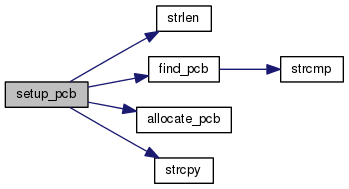
\includegraphics[width=334pt]{pcb_8c_aa8ef2e50138f1b01310c83d261c2efa9_cgraph}
\end{center}
\end{figure}




Here is the caller graph for this function\-:\nopagebreak
\begin{figure}[H]
\begin{center}
\leavevmode
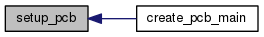
\includegraphics[width=270pt]{pcb_8c_aa8ef2e50138f1b01310c83d261c2efa9_icgraph}
\end{center}
\end{figure}


\hypertarget{pcb_8c_a094b4bf39d7297266e9b1336a233841e}{\index{pcb.\-c@{pcb.\-c}!show\-\_\-all\-\_\-processes@{show\-\_\-all\-\_\-processes}}
\index{show\-\_\-all\-\_\-processes@{show\-\_\-all\-\_\-processes}!pcb.c@{pcb.\-c}}
\subsubsection[{show\-\_\-all\-\_\-processes}]{\setlength{\rightskip}{0pt plus 5cm}void show\-\_\-all\-\_\-processes (
\begin{DoxyParamCaption}
{}
\end{DoxyParamCaption}
)}}\label{pcb_8c_a094b4bf39d7297266e9b1336a233841e}


Here is the call graph for this function\-:\nopagebreak
\begin{figure}[H]
\begin{center}
\leavevmode
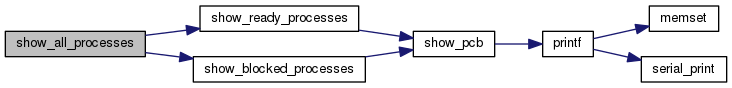
\includegraphics[width=350pt]{pcb_8c_a094b4bf39d7297266e9b1336a233841e_cgraph}
\end{center}
\end{figure}




Here is the caller graph for this function\-:\nopagebreak
\begin{figure}[H]
\begin{center}
\leavevmode
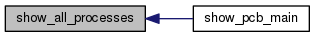
\includegraphics[width=310pt]{pcb_8c_a094b4bf39d7297266e9b1336a233841e_icgraph}
\end{center}
\end{figure}


\hypertarget{pcb_8c_a918cbc9698ab932896ec81c482fee9f1}{\index{pcb.\-c@{pcb.\-c}!show\-\_\-blocked\-\_\-processes@{show\-\_\-blocked\-\_\-processes}}
\index{show\-\_\-blocked\-\_\-processes@{show\-\_\-blocked\-\_\-processes}!pcb.c@{pcb.\-c}}
\subsubsection[{show\-\_\-blocked\-\_\-processes}]{\setlength{\rightskip}{0pt plus 5cm}void show\-\_\-blocked\-\_\-processes (
\begin{DoxyParamCaption}
{}
\end{DoxyParamCaption}
)}}\label{pcb_8c_a918cbc9698ab932896ec81c482fee9f1}


Here is the call graph for this function\-:\nopagebreak
\begin{figure}[H]
\begin{center}
\leavevmode
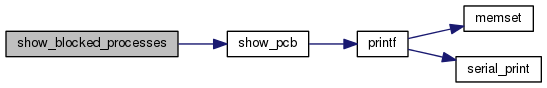
\includegraphics[width=350pt]{pcb_8c_a918cbc9698ab932896ec81c482fee9f1_cgraph}
\end{center}
\end{figure}




Here is the caller graph for this function\-:\nopagebreak
\begin{figure}[H]
\begin{center}
\leavevmode
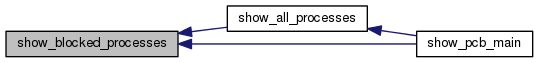
\includegraphics[width=350pt]{pcb_8c_a918cbc9698ab932896ec81c482fee9f1_icgraph}
\end{center}
\end{figure}


\hypertarget{pcb_8c_af08c093fa9ecf34738d5e295520a032a}{\index{pcb.\-c@{pcb.\-c}!show\-\_\-pcb@{show\-\_\-pcb}}
\index{show\-\_\-pcb@{show\-\_\-pcb}!pcb.c@{pcb.\-c}}
\subsubsection[{show\-\_\-pcb}]{\setlength{\rightskip}{0pt plus 5cm}{\bf error\-\_\-t} show\-\_\-pcb (
\begin{DoxyParamCaption}
\item[{struct {\bf pcb\-\_\-struct} $\ast$}]{pcb\-\_\-ptr}
\end{DoxyParamCaption}
)}}\label{pcb_8c_af08c093fa9ecf34738d5e295520a032a}


Here is the call graph for this function\-:\nopagebreak
\begin{figure}[H]
\begin{center}
\leavevmode
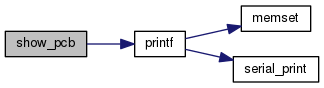
\includegraphics[width=316pt]{pcb_8c_af08c093fa9ecf34738d5e295520a032a_cgraph}
\end{center}
\end{figure}




Here is the caller graph for this function\-:\nopagebreak
\begin{figure}[H]
\begin{center}
\leavevmode
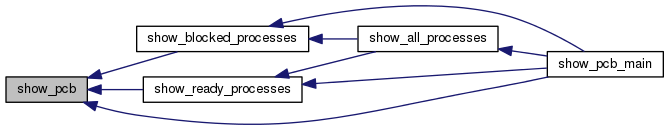
\includegraphics[width=350pt]{pcb_8c_af08c093fa9ecf34738d5e295520a032a_icgraph}
\end{center}
\end{figure}


\hypertarget{pcb_8c_a542627a44f5cbaf08ceaab05a419acee}{\index{pcb.\-c@{pcb.\-c}!show\-\_\-ready\-\_\-processes@{show\-\_\-ready\-\_\-processes}}
\index{show\-\_\-ready\-\_\-processes@{show\-\_\-ready\-\_\-processes}!pcb.c@{pcb.\-c}}
\subsubsection[{show\-\_\-ready\-\_\-processes}]{\setlength{\rightskip}{0pt plus 5cm}void show\-\_\-ready\-\_\-processes (
\begin{DoxyParamCaption}
{}
\end{DoxyParamCaption}
)}}\label{pcb_8c_a542627a44f5cbaf08ceaab05a419acee}


Here is the call graph for this function\-:\nopagebreak
\begin{figure}[H]
\begin{center}
\leavevmode
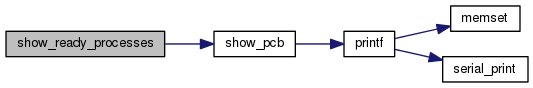
\includegraphics[width=350pt]{pcb_8c_a542627a44f5cbaf08ceaab05a419acee_cgraph}
\end{center}
\end{figure}




Here is the caller graph for this function\-:\nopagebreak
\begin{figure}[H]
\begin{center}
\leavevmode
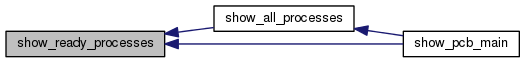
\includegraphics[width=350pt]{pcb_8c_a542627a44f5cbaf08ceaab05a419acee_icgraph}
\end{center}
\end{figure}


\hypertarget{pcb_8c_acb4a05dff84e0ad1777c1991f95be1e0}{\index{pcb.\-c@{pcb.\-c}!suspend\-\_\-pcb@{suspend\-\_\-pcb}}
\index{suspend\-\_\-pcb@{suspend\-\_\-pcb}!pcb.c@{pcb.\-c}}
\subsubsection[{suspend\-\_\-pcb}]{\setlength{\rightskip}{0pt plus 5cm}{\bf error\-\_\-t} suspend\-\_\-pcb (
\begin{DoxyParamCaption}
\item[{struct {\bf pcb\-\_\-struct} $\ast$}]{pcb\-\_\-ptr}
\end{DoxyParamCaption}
)}}\label{pcb_8c_acb4a05dff84e0ad1777c1991f95be1e0}


Here is the caller graph for this function\-:\nopagebreak
\begin{figure}[H]
\begin{center}
\leavevmode
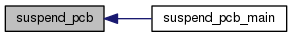
\includegraphics[width=292pt]{pcb_8c_acb4a05dff84e0ad1777c1991f95be1e0_icgraph}
\end{center}
\end{figure}


\hypertarget{pcb_8c_a0526b69c22b1961dad32f21f9b380f4b}{\index{pcb.\-c@{pcb.\-c}!unblock\-\_\-pcb@{unblock\-\_\-pcb}}
\index{unblock\-\_\-pcb@{unblock\-\_\-pcb}!pcb.c@{pcb.\-c}}
\subsubsection[{unblock\-\_\-pcb}]{\setlength{\rightskip}{0pt plus 5cm}{\bf error\-\_\-t} unblock\-\_\-pcb (
\begin{DoxyParamCaption}
\item[{struct {\bf pcb\-\_\-struct} $\ast$}]{pcb\-\_\-ptr}
\end{DoxyParamCaption}
)}}\label{pcb_8c_a0526b69c22b1961dad32f21f9b380f4b}


Here is the call graph for this function\-:\nopagebreak
\begin{figure}[H]
\begin{center}
\leavevmode
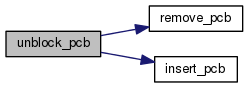
\includegraphics[width=258pt]{pcb_8c_a0526b69c22b1961dad32f21f9b380f4b_cgraph}
\end{center}
\end{figure}




Here is the caller graph for this function\-:\nopagebreak
\begin{figure}[H]
\begin{center}
\leavevmode
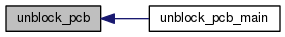
\includegraphics[width=286pt]{pcb_8c_a0526b69c22b1961dad32f21f9b380f4b_icgraph}
\end{center}
\end{figure}




\subsection{Variable Documentation}
\hypertarget{pcb_8c_a5e5a16f32884089aeed6b337440cf588}{\index{pcb.\-c@{pcb.\-c}!\-\_\-\-\_\-attribute\-\_\-\-\_\-@{\-\_\-\-\_\-attribute\-\_\-\-\_\-}}
\index{\-\_\-\-\_\-attribute\-\_\-\-\_\-@{\-\_\-\-\_\-attribute\-\_\-\-\_\-}!pcb.c@{pcb.\-c}}
\subsubsection[{\-\_\-\-\_\-attribute\-\_\-\-\_\-}]{\setlength{\rightskip}{0pt plus 5cm}enum {\bf process\-\_\-suspended} \-\_\-\-\_\-attribute\-\_\-\-\_\-}}\label{pcb_8c_a5e5a16f32884089aeed6b337440cf588}
\hypertarget{pcb_8c_a1faaaae288fc8ca4ed1751049aa2f84f}{\index{pcb.\-c@{pcb.\-c}!blocked@{blocked}}
\index{blocked@{blocked}!pcb.c@{pcb.\-c}}
\subsubsection[{blocked}]{\setlength{\rightskip}{0pt plus 5cm}blocked}}\label{pcb_8c_a1faaaae288fc8ca4ed1751049aa2f84f}


$<$ P\-C\-B in the blocked state. 

P\-C\-B in the blocked state.\hypertarget{pcb_8c_ae6c865df784842196d411c1466b01686}{\index{pcb.\-c@{pcb.\-c}!false@{false}}
\index{false@{false}!pcb.c@{pcb.\-c}}
\subsubsection[{false}]{\setlength{\rightskip}{0pt plus 5cm}false}}\label{pcb_8c_ae6c865df784842196d411c1466b01686}


$<$ P\-C\-B process is not suspended. 

P\-C\-B process is not suspended.\hypertarget{pcb_8c_ab0db378e6ced1decdb42263d4cb2789a}{\index{pcb.\-c@{pcb.\-c}!ready@{ready}}
\index{ready@{ready}!pcb.c@{pcb.\-c}}
\subsubsection[{ready}]{\setlength{\rightskip}{0pt plus 5cm}ready}}\label{pcb_8c_ab0db378e6ced1decdb42263d4cb2789a}


P\-C\-B in the ready state. 

\hypertarget{pcb_8c_a1a015fe02c9cea18a5cf62656e257c97}{\index{pcb.\-c@{pcb.\-c}!running@{running}}
\index{running@{running}!pcb.c@{pcb.\-c}}
\subsubsection[{running}]{\setlength{\rightskip}{0pt plus 5cm}running}}\label{pcb_8c_a1a015fe02c9cea18a5cf62656e257c97}


P\-C\-B in the running state. 

\hypertarget{pcb_8c_a1a24fc2eb8c1af6d06ac15bcec47f088}{\index{pcb.\-c@{pcb.\-c}!true@{true}}
\index{true@{true}!pcb.c@{pcb.\-c}}
\subsubsection[{true}]{\setlength{\rightskip}{0pt plus 5cm}true}}\label{pcb_8c_a1a24fc2eb8c1af6d06ac15bcec47f088}


P\-C\-B process is suspended. 


\hypertarget{pcb_8h}{\section{modules/r2/pcb.h File Reference}
\label{pcb_8h}\index{modules/r2/pcb.\-h@{modules/r2/pcb.\-h}}
}


The Process Control Block.  


{\ttfamily \#include \char`\"{}../errno.\-h\char`\"{}}\\*
Include dependency graph for pcb.\-h\-:\nopagebreak
\begin{figure}[H]
\begin{center}
\leavevmode
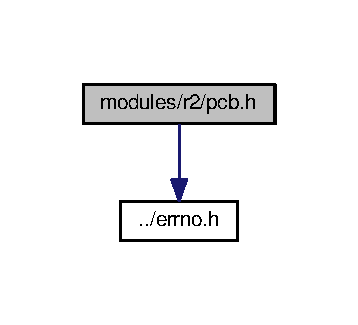
\includegraphics[width=172pt]{pcb_8h__incl}
\end{center}
\end{figure}
This graph shows which files directly or indirectly include this file\-:\nopagebreak
\begin{figure}[H]
\begin{center}
\leavevmode
\includegraphics[width=350pt]{pcb_8h__dep__incl}
\end{center}
\end{figure}
\subsection*{Macros}
\begin{DoxyCompactItemize}
\item 
\#define \hyperlink{pcb_8h_a417e28a8cf820ec6d8387986f8997e05}{S\-I\-Z\-E\-\_\-\-O\-F\-\_\-\-S\-T\-A\-C\-K}~1024
\end{DoxyCompactItemize}
\subsection*{Enumerations}
\begin{DoxyCompactItemize}
\item 
enum \hyperlink{pcb_8h_aefe309d62b55b4d0be96f1a97fcbbadd}{process\-\_\-class} 
\begin{DoxyCompactList}\small\item\em P\-C\-B process class types. \end{DoxyCompactList}\end{DoxyCompactItemize}
\subsection*{Functions}
\begin{DoxyCompactItemize}
\item 
enum \hyperlink{pcb_8h_aefe309d62b55b4d0be96f1a97fcbbadd}{process\-\_\-class} \hyperlink{pcb_8h_a54cfeca156d13fa2db0c7987bd5fb37a}{\-\_\-\-\_\-attribute\-\_\-\-\_\-} ((packed))
\end{DoxyCompactItemize}
\begin{Indent}{\bf pcb\-\_\-init}\par
{\em Initiates the P\-C\-B queues}\begin{DoxyCompactItemize}
\item 
void \hyperlink{pcb_8h_a8d00fee50178510712d2ffeaeafae347}{pcb\-\_\-init} ()
\end{DoxyCompactItemize}
\end{Indent}
\begin{Indent}{\bf allocate\-\_\-pcb}\par
{\em allocate a space for the P\-C\-B structure.

\begin{DoxyReturn}{Returns}
The pointer that point to the P\-C\-B structure. 
\end{DoxyReturn}
}\begin{DoxyCompactItemize}
\item 
struct \hyperlink{structpcb__struct}{pcb\-\_\-struct} $\ast$ \hyperlink{pcb_8h_a8fd9eebd60b5c6838b055b6dab7065e1}{allocate\-\_\-pcb} ()
\end{DoxyCompactItemize}
\end{Indent}
\begin{Indent}{\bf free\-\_\-pcb}\par
{\em Frees all memory associated with given P\-C\-B, including the P\-C\-B itself, the stack, etc, with sys\-\_\-free\-\_\-mem()


\begin{DoxyParams}{Parameters}
{\em pcb\-\_\-ptr} & The pointer to the P\-C\-B\\
\hline
\end{DoxyParams}
\begin{DoxyReturn}{Returns}
The error code. Possible error code to be returned\-: E\-\_\-\-N\-O\-E\-R\-R\-O\-R No error. E\-\_\-\-I\-N\-V\-P\-A\-R\-A The P\-C\-B probably had not been removed from queue before free it. 
\end{DoxyReturn}
}\begin{DoxyCompactItemize}
\item 
\hyperlink{errno_8h_aafbeb34410283829794b35fedafeb369}{error\-\_\-t} \hyperlink{pcb_8h_a31e603695448c5bd7bccacce5988eaf2}{free\-\_\-pcb} (struct \hyperlink{structpcb__struct}{pcb\-\_\-struct} $\ast$pcb\-\_\-ptr)
\end{DoxyCompactItemize}
\end{Indent}
\begin{Indent}{\bf setup\-\_\-pcb}\par
{\em allocate a space for the P\-C\-B structure, setup the properties of the P\-C\-B.

N\-O\-T\-E\-: p\-Name must less than 10 character, p\-Class should be either \char`\"{}application\char`\"{} or \char`\"{}system\char`\"{} , and p\-Priority must within the range of \mbox{[}0, 9\mbox{]}.


\begin{DoxyParams}{Parameters}
{\em p\-Name} & Process Name (length $<$ 10). \\
\hline
{\em p\-Class} & Process class (system or application). \\
\hline
{\em p\-Priority} & Process priority (0 $\sim$ 9).\\
\hline
\end{DoxyParams}
\begin{DoxyReturn}{Returns}
N\-U\-L\-L if error occured, otherwise, the pointer that point to the P\-C\-B structure. 
\end{DoxyReturn}
}\begin{DoxyCompactItemize}
\item 
struct \hyperlink{structpcb__struct}{pcb\-\_\-struct} $\ast$ \hyperlink{pcb_8h_aa8ef2e50138f1b01310c83d261c2efa9}{setup\-\_\-pcb} (const char $\ast$p\-Name, const enum \hyperlink{pcb_8h_aefe309d62b55b4d0be96f1a97fcbbadd}{process\-\_\-class} p\-Class, const unsigned char p\-Priority)
\end{DoxyCompactItemize}
\end{Indent}
\begin{Indent}{\bf find\-\_\-pcb}\par
{\em Will search all queues for a process named p\-Name


\begin{DoxyParams}{Parameters}
{\em p\-Name} & The char pointer to the desired searched name\\
\hline
\end{DoxyParams}
\begin{DoxyReturn}{Returns}
P\-C\-B pointer if found, N\-U\-L\-L if P\-C\-B is not found 
\end{DoxyReturn}
}\begin{DoxyCompactItemize}
\item 
struct \hyperlink{structpcb__struct}{pcb\-\_\-struct} $\ast$ \hyperlink{pcb_8h_acfbb91c24a4b3cdc22d9a27df468013d}{find\-\_\-pcb} (const char $\ast$p\-Name)
\end{DoxyCompactItemize}
\end{Indent}
\begin{Indent}{\bf insert\-\_\-pcb}\par
{\em Inserts P\-C\-B into the appropriate queue.


\begin{DoxyParams}{Parameters}
{\em pcb\-\_\-ptr} & The pointer to the P\-C\-B\\
\hline
\end{DoxyParams}
\begin{DoxyReturn}{Returns}
The error code. Possible error code to be returned\-: E\-\_\-\-N\-O\-E\-R\-R\-O\-R No error. E\-\_\-\-N\-U\-L\-L\-\_\-\-P\-T\-R Null pointer error. E\-\_\-\-I\-N\-V\-P\-A\-R\-A The given P\-C\-B has running status or abnormal data members. 
\end{DoxyReturn}
}\begin{DoxyCompactItemize}
\item 
\hyperlink{errno_8h_aafbeb34410283829794b35fedafeb369}{error\-\_\-t} \hyperlink{pcb_8h_ae8f8cca202f2232d4396a48db14b7d35}{insert\-\_\-pcb} (struct \hyperlink{structpcb__struct}{pcb\-\_\-struct} $\ast$pcb\-\_\-ptr)
\end{DoxyCompactItemize}
\end{Indent}
\begin{Indent}{\bf remove\-\_\-pcb}\par
{\em Removes P\-C\-B from the queue it is currently in.


\begin{DoxyParams}{Parameters}
{\em pcb\-\_\-ptr} & The pointer to the P\-C\-B\\
\hline
\end{DoxyParams}
\begin{DoxyReturn}{Returns}
The error code. Possible error code to be returned\-: E\-\_\-\-N\-O\-E\-R\-R\-O\-R No error. E\-\_\-\-N\-U\-L\-L\-\_\-\-P\-T\-R Null pointer error. E\-\_\-\-I\-N\-V\-P\-A\-R\-A The given P\-C\-B has abnormal data members. 
\end{DoxyReturn}
}\begin{DoxyCompactItemize}
\item 
\hyperlink{errno_8h_aafbeb34410283829794b35fedafeb369}{error\-\_\-t} \hyperlink{pcb_8h_a52620da5c66ed459beea65538169547a}{remove\-\_\-pcb} (struct \hyperlink{structpcb__struct}{pcb\-\_\-struct} $\ast$pcb\-\_\-ptr)
\end{DoxyCompactItemize}
\end{Indent}
\begin{Indent}{\bf suspend\-\_\-pcb}\par
{\em Suspends the specific P\-C\-B.


\begin{DoxyParams}{Parameters}
{\em pcb\-\_\-ptr} & The pointer to the P\-C\-B\\
\hline
\end{DoxyParams}
\begin{DoxyReturn}{Returns}
The error code. Possible error code to be returned\-: E\-\_\-\-N\-O\-E\-R\-R\-O\-R No error. E\-\_\-\-N\-U\-L\-L\-\_\-\-P\-T\-R Null pointer error. 
\end{DoxyReturn}
}\begin{DoxyCompactItemize}
\item 
\hyperlink{errno_8h_aafbeb34410283829794b35fedafeb369}{error\-\_\-t} \hyperlink{pcb_8h_acb4a05dff84e0ad1777c1991f95be1e0}{suspend\-\_\-pcb} (struct \hyperlink{structpcb__struct}{pcb\-\_\-struct} $\ast$pcb\-\_\-ptr)
\end{DoxyCompactItemize}
\end{Indent}
\begin{Indent}{\bf resume\-\_\-pcb}\par
{\em Resumes the specific P\-C\-B.


\begin{DoxyParams}{Parameters}
{\em pcb\-\_\-ptr} & The pointer to the P\-C\-B\\
\hline
\end{DoxyParams}
\begin{DoxyReturn}{Returns}
The error code. Possible error code to be returned\-: E\-\_\-\-N\-O\-E\-R\-R\-O\-R No error. E\-\_\-\-N\-U\-L\-L\-\_\-\-P\-T\-R Null pointer error. 
\end{DoxyReturn}
}\begin{DoxyCompactItemize}
\item 
\hyperlink{errno_8h_aafbeb34410283829794b35fedafeb369}{error\-\_\-t} \hyperlink{pcb_8h_a24a874ae323c9ef0583c2f179b44fe74}{resume\-\_\-pcb} (struct \hyperlink{structpcb__struct}{pcb\-\_\-struct} $\ast$pcb\-\_\-ptr)
\end{DoxyCompactItemize}
\end{Indent}
\begin{Indent}{\bf set\-\_\-pcb\-\_\-priority}\par
{\em Sets the priority of the selected P\-C\-B


\begin{DoxyParams}{Parameters}
{\em pcb\-\_\-ptr} & The P\-C\-B pointer. \\
\hline
{\em p\-Priorty} & The assigned priorirty \\
\hline
\end{DoxyParams}
\begin{DoxyReturn}{Returns}
The error code. Possible error code to be returned\-: E\-\_\-\-N\-O\-E\-R\-R\-O\-R No error. E\-\_\-\-N\-U\-L\-L\-\_\-\-P\-T\-R Null pointer error. E\-\_\-\-I\-N\-V\-P\-A\-R\-A The p\-Priority is out of range. Or, the given P\-C\-B has abnormal data members (By \char`\"{}remove\-\_\-pcb\char`\"{} or \char`\"{}insert\-\_\-pcb\char`\"{}). 
\end{DoxyReturn}
}\begin{DoxyCompactItemize}
\item 
\hyperlink{errno_8h_aafbeb34410283829794b35fedafeb369}{error\-\_\-t} \hyperlink{pcb_8h_a863d9b3d5113d72ebc7b64e01937fc97}{set\-\_\-pcb\-\_\-priority} (struct \hyperlink{structpcb__struct}{pcb\-\_\-struct} $\ast$pcb\-\_\-ptr, const unsigned char p\-Priority)
\end{DoxyCompactItemize}
\end{Indent}
\begin{Indent}{\bf show\-\_\-pcb}\par
{\em Displays the name, class, state, suspend status, and priority of a P\-C\-B.


\begin{DoxyParams}{Parameters}
{\em p\-Name} & The P\-C\-B pointer. \\
\hline
\end{DoxyParams}
\begin{DoxyReturn}{Returns}
The error code. Possible error code to be returned\-: E\-\_\-\-N\-O\-E\-R\-R\-O\-R No error. E\-\_\-\-N\-U\-L\-L\-\_\-\-P\-T\-R Null pointer error. 
\end{DoxyReturn}
}\begin{DoxyCompactItemize}
\item 
\hyperlink{errno_8h_aafbeb34410283829794b35fedafeb369}{error\-\_\-t} \hyperlink{pcb_8h_af08c093fa9ecf34738d5e295520a032a}{show\-\_\-pcb} (struct \hyperlink{structpcb__struct}{pcb\-\_\-struct} $\ast$pcb\-\_\-ptr)
\end{DoxyCompactItemize}
\end{Indent}
\begin{Indent}{\bf show\-\_\-all\-\_\-processes}\par
{\em Displays all of the processes and their attributes.

\begin{DoxyReturn}{Returns}
V\-O\-I\-D. 
\end{DoxyReturn}
}\begin{DoxyCompactItemize}
\item 
void \hyperlink{pcb_8h_a094b4bf39d7297266e9b1336a233841e}{show\-\_\-all\-\_\-processes} ()
\end{DoxyCompactItemize}
\end{Indent}
\begin{Indent}{\bf show\-\_\-ready\-\_\-processes}\par
{\em Displays all of the ready processes and their attributes.

\begin{DoxyReturn}{Returns}
V\-O\-I\-D. 
\end{DoxyReturn}
}\begin{DoxyCompactItemize}
\item 
void \hyperlink{pcb_8h_a542627a44f5cbaf08ceaab05a419acee}{show\-\_\-ready\-\_\-processes} ()
\end{DoxyCompactItemize}
\end{Indent}
\begin{Indent}{\bf show\-\_\-blocked\-\_\-processes}\par
{\em displays all blocked processes and their attributes

\begin{DoxyReturn}{Returns}
V\-O\-I\-D. 
\end{DoxyReturn}
}\begin{DoxyCompactItemize}
\item 
void \hyperlink{pcb_8h_a918cbc9698ab932896ec81c482fee9f1}{show\-\_\-blocked\-\_\-processes} ()
\end{DoxyCompactItemize}
\end{Indent}
\begin{Indent}{\bf block\-\_\-pcb}\par
{\em puts the given pcb into the blocked state and places it into the correct queue


\begin{DoxyParams}{Parameters}
{\em pcb\-\_\-ptr} & The pointer to the P\-C\-B\\
\hline
\end{DoxyParams}
\begin{DoxyReturn}{Returns}
The error code. Possible error code to be returned\-: E\-\_\-\-N\-O\-E\-R\-R\-O\-R No error. E\-\_\-\-N\-U\-L\-L\-\_\-\-P\-T\-R Null pointer error. E\-\_\-\-I\-N\-V\-P\-A\-R\-A The given P\-C\-B has abnormal data members (By \char`\"{}remove\-\_\-pcb\char`\"{} or \char`\"{}insert\-\_\-pcb\char`\"{}). 
\end{DoxyReturn}
}\begin{DoxyCompactItemize}
\item 
\hyperlink{errno_8h_aafbeb34410283829794b35fedafeb369}{error\-\_\-t} \hyperlink{pcb_8h_aa5aad077eb0c15c0c76fc4522b11a410}{block\-\_\-pcb} (struct \hyperlink{structpcb__struct}{pcb\-\_\-struct} $\ast$pcb\-\_\-ptr)
\end{DoxyCompactItemize}
\end{Indent}
\begin{Indent}{\bf unblock\-\_\-pcb}\par
{\em puts the given pcb into the unblocked state and places it into the correct queue


\begin{DoxyParams}{Parameters}
{\em pcb\-\_\-ptr} & The pointer to the P\-C\-B\\
\hline
\end{DoxyParams}
\begin{DoxyReturn}{Returns}
The error code. Possible error code to be returned\-: E\-\_\-\-N\-O\-E\-R\-R\-O\-R No error. E\-\_\-\-N\-U\-L\-L\-\_\-\-P\-T\-R Null pointer error. E\-\_\-\-I\-N\-V\-P\-A\-R\-A The given P\-C\-B has abnormal data members (By \char`\"{}remove\-\_\-pcb\char`\"{} or \char`\"{}insert\-\_\-pcb\char`\"{}). 
\end{DoxyReturn}
}\begin{DoxyCompactItemize}
\item 
\hyperlink{errno_8h_aafbeb34410283829794b35fedafeb369}{error\-\_\-t} \hyperlink{pcb_8h_a0526b69c22b1961dad32f21f9b380f4b}{unblock\-\_\-pcb} (struct \hyperlink{structpcb__struct}{pcb\-\_\-struct} $\ast$pcb\-\_\-ptr)
\end{DoxyCompactItemize}
\end{Indent}
\subsection*{Variables}
\begin{DoxyCompactItemize}
\item 
\hyperlink{pcb_8h_a43f5eb2fcb8f17fcfd4bb0f9bebb72e6}{pcb\-\_\-class\-\_\-app}
\begin{DoxyCompactList}\small\item\em Process is an application process. \end{DoxyCompactList}\item 
\hyperlink{pcb_8h_ad04b9d9c8a14430bd83833ab0e8476fd}{pcb\-\_\-class\-\_\-sys}
\begin{DoxyCompactList}\small\item\em $<$ Process is a system process. \end{DoxyCompactList}\end{DoxyCompactItemize}


\subsection{Detailed Description}
The Process Control Block. \begin{DoxyAuthor}{Author}
Thunder Krakens 
\end{DoxyAuthor}
\begin{DoxyDate}{Date}
February 7th, 2016 
\end{DoxyDate}
\begin{DoxyVersion}{Version}
R2 
\end{DoxyVersion}


\subsection{Macro Definition Documentation}
\hypertarget{pcb_8h_a417e28a8cf820ec6d8387986f8997e05}{\index{pcb.\-h@{pcb.\-h}!S\-I\-Z\-E\-\_\-\-O\-F\-\_\-\-S\-T\-A\-C\-K@{S\-I\-Z\-E\-\_\-\-O\-F\-\_\-\-S\-T\-A\-C\-K}}
\index{S\-I\-Z\-E\-\_\-\-O\-F\-\_\-\-S\-T\-A\-C\-K@{S\-I\-Z\-E\-\_\-\-O\-F\-\_\-\-S\-T\-A\-C\-K}!pcb.h@{pcb.\-h}}
\subsubsection[{S\-I\-Z\-E\-\_\-\-O\-F\-\_\-\-S\-T\-A\-C\-K}]{\setlength{\rightskip}{0pt plus 5cm}\#define S\-I\-Z\-E\-\_\-\-O\-F\-\_\-\-S\-T\-A\-C\-K~1024}}\label{pcb_8h_a417e28a8cf820ec6d8387986f8997e05}


\subsection{Enumeration Type Documentation}
\hypertarget{pcb_8h_aefe309d62b55b4d0be96f1a97fcbbadd}{\index{pcb.\-h@{pcb.\-h}!process\-\_\-class@{process\-\_\-class}}
\index{process\-\_\-class@{process\-\_\-class}!pcb.h@{pcb.\-h}}
\subsubsection[{process\-\_\-class}]{\setlength{\rightskip}{0pt plus 5cm}enum {\bf process\-\_\-class}}}\label{pcb_8h_aefe309d62b55b4d0be96f1a97fcbbadd}


P\-C\-B process class types. 



\subsection{Function Documentation}
\hypertarget{pcb_8h_a54cfeca156d13fa2db0c7987bd5fb37a}{\index{pcb.\-h@{pcb.\-h}!\-\_\-\-\_\-attribute\-\_\-\-\_\-@{\-\_\-\-\_\-attribute\-\_\-\-\_\-}}
\index{\-\_\-\-\_\-attribute\-\_\-\-\_\-@{\-\_\-\-\_\-attribute\-\_\-\-\_\-}!pcb.h@{pcb.\-h}}
\subsubsection[{\-\_\-\-\_\-attribute\-\_\-\-\_\-}]{\setlength{\rightskip}{0pt plus 5cm}enum {\bf process\-\_\-class} \-\_\-\-\_\-attribute\-\_\-\-\_\- (
\begin{DoxyParamCaption}
\item[{(packed)}]{}
\end{DoxyParamCaption}
)}}\label{pcb_8h_a54cfeca156d13fa2db0c7987bd5fb37a}
\hypertarget{pcb_8h_a8fd9eebd60b5c6838b055b6dab7065e1}{\index{pcb.\-h@{pcb.\-h}!allocate\-\_\-pcb@{allocate\-\_\-pcb}}
\index{allocate\-\_\-pcb@{allocate\-\_\-pcb}!pcb.h@{pcb.\-h}}
\subsubsection[{allocate\-\_\-pcb}]{\setlength{\rightskip}{0pt plus 5cm}struct {\bf pcb\-\_\-struct}$\ast$ allocate\-\_\-pcb (
\begin{DoxyParamCaption}
{}
\end{DoxyParamCaption}
)}}\label{pcb_8h_a8fd9eebd60b5c6838b055b6dab7065e1}


Here is the caller graph for this function\-:\nopagebreak
\begin{figure}[H]
\begin{center}
\leavevmode
\includegraphics[width=350pt]{pcb_8h_a8fd9eebd60b5c6838b055b6dab7065e1_icgraph}
\end{center}
\end{figure}


\hypertarget{pcb_8h_aa5aad077eb0c15c0c76fc4522b11a410}{\index{pcb.\-h@{pcb.\-h}!block\-\_\-pcb@{block\-\_\-pcb}}
\index{block\-\_\-pcb@{block\-\_\-pcb}!pcb.h@{pcb.\-h}}
\subsubsection[{block\-\_\-pcb}]{\setlength{\rightskip}{0pt plus 5cm}{\bf error\-\_\-t} block\-\_\-pcb (
\begin{DoxyParamCaption}
\item[{struct {\bf pcb\-\_\-struct} $\ast$}]{pcb\-\_\-ptr}
\end{DoxyParamCaption}
)}}\label{pcb_8h_aa5aad077eb0c15c0c76fc4522b11a410}


Here is the call graph for this function\-:\nopagebreak
\begin{figure}[H]
\begin{center}
\leavevmode
\includegraphics[width=248pt]{pcb_8h_aa5aad077eb0c15c0c76fc4522b11a410_cgraph}
\end{center}
\end{figure}




Here is the caller graph for this function\-:\nopagebreak
\begin{figure}[H]
\begin{center}
\leavevmode
\includegraphics[width=266pt]{pcb_8h_aa5aad077eb0c15c0c76fc4522b11a410_icgraph}
\end{center}
\end{figure}


\hypertarget{pcb_8h_acfbb91c24a4b3cdc22d9a27df468013d}{\index{pcb.\-h@{pcb.\-h}!find\-\_\-pcb@{find\-\_\-pcb}}
\index{find\-\_\-pcb@{find\-\_\-pcb}!pcb.h@{pcb.\-h}}
\subsubsection[{find\-\_\-pcb}]{\setlength{\rightskip}{0pt plus 5cm}struct {\bf pcb\-\_\-struct}$\ast$ find\-\_\-pcb (
\begin{DoxyParamCaption}
\item[{const char $\ast$}]{p\-Name}
\end{DoxyParamCaption}
)}}\label{pcb_8h_acfbb91c24a4b3cdc22d9a27df468013d}


Here is the call graph for this function\-:\nopagebreak
\begin{figure}[H]
\begin{center}
\leavevmode
\includegraphics[width=218pt]{pcb_8h_acfbb91c24a4b3cdc22d9a27df468013d_cgraph}
\end{center}
\end{figure}




Here is the caller graph for this function\-:\nopagebreak
\begin{figure}[H]
\begin{center}
\leavevmode
\includegraphics[width=350pt]{pcb_8h_acfbb91c24a4b3cdc22d9a27df468013d_icgraph}
\end{center}
\end{figure}


\hypertarget{pcb_8h_a31e603695448c5bd7bccacce5988eaf2}{\index{pcb.\-h@{pcb.\-h}!free\-\_\-pcb@{free\-\_\-pcb}}
\index{free\-\_\-pcb@{free\-\_\-pcb}!pcb.h@{pcb.\-h}}
\subsubsection[{free\-\_\-pcb}]{\setlength{\rightskip}{0pt plus 5cm}{\bf error\-\_\-t} free\-\_\-pcb (
\begin{DoxyParamCaption}
\item[{struct {\bf pcb\-\_\-struct} $\ast$}]{pcb\-\_\-ptr}
\end{DoxyParamCaption}
)}}\label{pcb_8h_a31e603695448c5bd7bccacce5988eaf2}


Here is the caller graph for this function\-:\nopagebreak
\begin{figure}[H]
\begin{center}
\leavevmode
\includegraphics[width=260pt]{pcb_8h_a31e603695448c5bd7bccacce5988eaf2_icgraph}
\end{center}
\end{figure}


\hypertarget{pcb_8h_ae8f8cca202f2232d4396a48db14b7d35}{\index{pcb.\-h@{pcb.\-h}!insert\-\_\-pcb@{insert\-\_\-pcb}}
\index{insert\-\_\-pcb@{insert\-\_\-pcb}!pcb.h@{pcb.\-h}}
\subsubsection[{insert\-\_\-pcb}]{\setlength{\rightskip}{0pt plus 5cm}{\bf error\-\_\-t} insert\-\_\-pcb (
\begin{DoxyParamCaption}
\item[{struct {\bf pcb\-\_\-struct} $\ast$}]{pcb\-\_\-ptr}
\end{DoxyParamCaption}
)}}\label{pcb_8h_ae8f8cca202f2232d4396a48db14b7d35}


Here is the caller graph for this function\-:\nopagebreak
\begin{figure}[H]
\begin{center}
\leavevmode
\includegraphics[width=350pt]{pcb_8h_ae8f8cca202f2232d4396a48db14b7d35_icgraph}
\end{center}
\end{figure}


\hypertarget{pcb_8h_a8d00fee50178510712d2ffeaeafae347}{\index{pcb.\-h@{pcb.\-h}!pcb\-\_\-init@{pcb\-\_\-init}}
\index{pcb\-\_\-init@{pcb\-\_\-init}!pcb.h@{pcb.\-h}}
\subsubsection[{pcb\-\_\-init}]{\setlength{\rightskip}{0pt plus 5cm}void pcb\-\_\-init (
\begin{DoxyParamCaption}
{}
\end{DoxyParamCaption}
)}}\label{pcb_8h_a8d00fee50178510712d2ffeaeafae347}
\hypertarget{pcb_8h_a52620da5c66ed459beea65538169547a}{\index{pcb.\-h@{pcb.\-h}!remove\-\_\-pcb@{remove\-\_\-pcb}}
\index{remove\-\_\-pcb@{remove\-\_\-pcb}!pcb.h@{pcb.\-h}}
\subsubsection[{remove\-\_\-pcb}]{\setlength{\rightskip}{0pt plus 5cm}{\bf error\-\_\-t} remove\-\_\-pcb (
\begin{DoxyParamCaption}
\item[{struct {\bf pcb\-\_\-struct} $\ast$}]{pcb\-\_\-ptr}
\end{DoxyParamCaption}
)}}\label{pcb_8h_a52620da5c66ed459beea65538169547a}


Here is the caller graph for this function\-:\nopagebreak
\begin{figure}[H]
\begin{center}
\leavevmode
\includegraphics[width=350pt]{pcb_8h_a52620da5c66ed459beea65538169547a_icgraph}
\end{center}
\end{figure}


\hypertarget{pcb_8h_a24a874ae323c9ef0583c2f179b44fe74}{\index{pcb.\-h@{pcb.\-h}!resume\-\_\-pcb@{resume\-\_\-pcb}}
\index{resume\-\_\-pcb@{resume\-\_\-pcb}!pcb.h@{pcb.\-h}}
\subsubsection[{resume\-\_\-pcb}]{\setlength{\rightskip}{0pt plus 5cm}{\bf error\-\_\-t} resume\-\_\-pcb (
\begin{DoxyParamCaption}
\item[{struct {\bf pcb\-\_\-struct} $\ast$}]{pcb\-\_\-ptr}
\end{DoxyParamCaption}
)}}\label{pcb_8h_a24a874ae323c9ef0583c2f179b44fe74}


Here is the caller graph for this function\-:\nopagebreak
\begin{figure}[H]
\begin{center}
\leavevmode
\includegraphics[width=282pt]{pcb_8h_a24a874ae323c9ef0583c2f179b44fe74_icgraph}
\end{center}
\end{figure}


\hypertarget{pcb_8h_a863d9b3d5113d72ebc7b64e01937fc97}{\index{pcb.\-h@{pcb.\-h}!set\-\_\-pcb\-\_\-priority@{set\-\_\-pcb\-\_\-priority}}
\index{set\-\_\-pcb\-\_\-priority@{set\-\_\-pcb\-\_\-priority}!pcb.h@{pcb.\-h}}
\subsubsection[{set\-\_\-pcb\-\_\-priority}]{\setlength{\rightskip}{0pt plus 5cm}{\bf error\-\_\-t} set\-\_\-pcb\-\_\-priority (
\begin{DoxyParamCaption}
\item[{struct {\bf pcb\-\_\-struct} $\ast$}]{pcb\-\_\-ptr, }
\item[{const unsigned char}]{p\-Priority}
\end{DoxyParamCaption}
)}}\label{pcb_8h_a863d9b3d5113d72ebc7b64e01937fc97}


Here is the call graph for this function\-:\nopagebreak
\begin{figure}[H]
\begin{center}
\leavevmode
\includegraphics[width=272pt]{pcb_8h_a863d9b3d5113d72ebc7b64e01937fc97_cgraph}
\end{center}
\end{figure}




Here is the caller graph for this function\-:\nopagebreak
\begin{figure}[H]
\begin{center}
\leavevmode
\includegraphics[width=314pt]{pcb_8h_a863d9b3d5113d72ebc7b64e01937fc97_icgraph}
\end{center}
\end{figure}


\hypertarget{pcb_8h_aa8ef2e50138f1b01310c83d261c2efa9}{\index{pcb.\-h@{pcb.\-h}!setup\-\_\-pcb@{setup\-\_\-pcb}}
\index{setup\-\_\-pcb@{setup\-\_\-pcb}!pcb.h@{pcb.\-h}}
\subsubsection[{setup\-\_\-pcb}]{\setlength{\rightskip}{0pt plus 5cm}struct {\bf pcb\-\_\-struct}$\ast$ setup\-\_\-pcb (
\begin{DoxyParamCaption}
\item[{const char $\ast$}]{p\-Name, }
\item[{const enum {\bf process\-\_\-class}}]{p\-Class, }
\item[{const unsigned char}]{p\-Priority}
\end{DoxyParamCaption}
)}}\label{pcb_8h_aa8ef2e50138f1b01310c83d261c2efa9}


Here is the call graph for this function\-:\nopagebreak
\begin{figure}[H]
\begin{center}
\leavevmode
\includegraphics[width=334pt]{pcb_8h_aa8ef2e50138f1b01310c83d261c2efa9_cgraph}
\end{center}
\end{figure}




Here is the caller graph for this function\-:\nopagebreak
\begin{figure}[H]
\begin{center}
\leavevmode
\includegraphics[width=270pt]{pcb_8h_aa8ef2e50138f1b01310c83d261c2efa9_icgraph}
\end{center}
\end{figure}


\hypertarget{pcb_8h_a094b4bf39d7297266e9b1336a233841e}{\index{pcb.\-h@{pcb.\-h}!show\-\_\-all\-\_\-processes@{show\-\_\-all\-\_\-processes}}
\index{show\-\_\-all\-\_\-processes@{show\-\_\-all\-\_\-processes}!pcb.h@{pcb.\-h}}
\subsubsection[{show\-\_\-all\-\_\-processes}]{\setlength{\rightskip}{0pt plus 5cm}void show\-\_\-all\-\_\-processes (
\begin{DoxyParamCaption}
{}
\end{DoxyParamCaption}
)}}\label{pcb_8h_a094b4bf39d7297266e9b1336a233841e}


Here is the call graph for this function\-:\nopagebreak
\begin{figure}[H]
\begin{center}
\leavevmode
\includegraphics[width=350pt]{pcb_8h_a094b4bf39d7297266e9b1336a233841e_cgraph}
\end{center}
\end{figure}




Here is the caller graph for this function\-:\nopagebreak
\begin{figure}[H]
\begin{center}
\leavevmode
\includegraphics[width=310pt]{pcb_8h_a094b4bf39d7297266e9b1336a233841e_icgraph}
\end{center}
\end{figure}


\hypertarget{pcb_8h_a918cbc9698ab932896ec81c482fee9f1}{\index{pcb.\-h@{pcb.\-h}!show\-\_\-blocked\-\_\-processes@{show\-\_\-blocked\-\_\-processes}}
\index{show\-\_\-blocked\-\_\-processes@{show\-\_\-blocked\-\_\-processes}!pcb.h@{pcb.\-h}}
\subsubsection[{show\-\_\-blocked\-\_\-processes}]{\setlength{\rightskip}{0pt plus 5cm}void show\-\_\-blocked\-\_\-processes (
\begin{DoxyParamCaption}
{}
\end{DoxyParamCaption}
)}}\label{pcb_8h_a918cbc9698ab932896ec81c482fee9f1}


Here is the call graph for this function\-:\nopagebreak
\begin{figure}[H]
\begin{center}
\leavevmode
\includegraphics[width=350pt]{pcb_8h_a918cbc9698ab932896ec81c482fee9f1_cgraph}
\end{center}
\end{figure}




Here is the caller graph for this function\-:\nopagebreak
\begin{figure}[H]
\begin{center}
\leavevmode
\includegraphics[width=350pt]{pcb_8h_a918cbc9698ab932896ec81c482fee9f1_icgraph}
\end{center}
\end{figure}


\hypertarget{pcb_8h_af08c093fa9ecf34738d5e295520a032a}{\index{pcb.\-h@{pcb.\-h}!show\-\_\-pcb@{show\-\_\-pcb}}
\index{show\-\_\-pcb@{show\-\_\-pcb}!pcb.h@{pcb.\-h}}
\subsubsection[{show\-\_\-pcb}]{\setlength{\rightskip}{0pt plus 5cm}{\bf error\-\_\-t} show\-\_\-pcb (
\begin{DoxyParamCaption}
\item[{struct {\bf pcb\-\_\-struct} $\ast$}]{pcb\-\_\-ptr}
\end{DoxyParamCaption}
)}}\label{pcb_8h_af08c093fa9ecf34738d5e295520a032a}


Here is the call graph for this function\-:\nopagebreak
\begin{figure}[H]
\begin{center}
\leavevmode
\includegraphics[width=316pt]{pcb_8h_af08c093fa9ecf34738d5e295520a032a_cgraph}
\end{center}
\end{figure}




Here is the caller graph for this function\-:\nopagebreak
\begin{figure}[H]
\begin{center}
\leavevmode
\includegraphics[width=350pt]{pcb_8h_af08c093fa9ecf34738d5e295520a032a_icgraph}
\end{center}
\end{figure}


\hypertarget{pcb_8h_a542627a44f5cbaf08ceaab05a419acee}{\index{pcb.\-h@{pcb.\-h}!show\-\_\-ready\-\_\-processes@{show\-\_\-ready\-\_\-processes}}
\index{show\-\_\-ready\-\_\-processes@{show\-\_\-ready\-\_\-processes}!pcb.h@{pcb.\-h}}
\subsubsection[{show\-\_\-ready\-\_\-processes}]{\setlength{\rightskip}{0pt plus 5cm}void show\-\_\-ready\-\_\-processes (
\begin{DoxyParamCaption}
{}
\end{DoxyParamCaption}
)}}\label{pcb_8h_a542627a44f5cbaf08ceaab05a419acee}


Here is the call graph for this function\-:\nopagebreak
\begin{figure}[H]
\begin{center}
\leavevmode
\includegraphics[width=350pt]{pcb_8h_a542627a44f5cbaf08ceaab05a419acee_cgraph}
\end{center}
\end{figure}




Here is the caller graph for this function\-:\nopagebreak
\begin{figure}[H]
\begin{center}
\leavevmode
\includegraphics[width=350pt]{pcb_8h_a542627a44f5cbaf08ceaab05a419acee_icgraph}
\end{center}
\end{figure}


\hypertarget{pcb_8h_acb4a05dff84e0ad1777c1991f95be1e0}{\index{pcb.\-h@{pcb.\-h}!suspend\-\_\-pcb@{suspend\-\_\-pcb}}
\index{suspend\-\_\-pcb@{suspend\-\_\-pcb}!pcb.h@{pcb.\-h}}
\subsubsection[{suspend\-\_\-pcb}]{\setlength{\rightskip}{0pt plus 5cm}{\bf error\-\_\-t} suspend\-\_\-pcb (
\begin{DoxyParamCaption}
\item[{struct {\bf pcb\-\_\-struct} $\ast$}]{pcb\-\_\-ptr}
\end{DoxyParamCaption}
)}}\label{pcb_8h_acb4a05dff84e0ad1777c1991f95be1e0}


Here is the caller graph for this function\-:\nopagebreak
\begin{figure}[H]
\begin{center}
\leavevmode
\includegraphics[width=292pt]{pcb_8h_acb4a05dff84e0ad1777c1991f95be1e0_icgraph}
\end{center}
\end{figure}


\hypertarget{pcb_8h_a0526b69c22b1961dad32f21f9b380f4b}{\index{pcb.\-h@{pcb.\-h}!unblock\-\_\-pcb@{unblock\-\_\-pcb}}
\index{unblock\-\_\-pcb@{unblock\-\_\-pcb}!pcb.h@{pcb.\-h}}
\subsubsection[{unblock\-\_\-pcb}]{\setlength{\rightskip}{0pt plus 5cm}{\bf error\-\_\-t} unblock\-\_\-pcb (
\begin{DoxyParamCaption}
\item[{struct {\bf pcb\-\_\-struct} $\ast$}]{pcb\-\_\-ptr}
\end{DoxyParamCaption}
)}}\label{pcb_8h_a0526b69c22b1961dad32f21f9b380f4b}


Here is the call graph for this function\-:\nopagebreak
\begin{figure}[H]
\begin{center}
\leavevmode
\includegraphics[width=258pt]{pcb_8h_a0526b69c22b1961dad32f21f9b380f4b_cgraph}
\end{center}
\end{figure}




Here is the caller graph for this function\-:\nopagebreak
\begin{figure}[H]
\begin{center}
\leavevmode
\includegraphics[width=286pt]{pcb_8h_a0526b69c22b1961dad32f21f9b380f4b_icgraph}
\end{center}
\end{figure}




\subsection{Variable Documentation}
\hypertarget{pcb_8h_a43f5eb2fcb8f17fcfd4bb0f9bebb72e6}{\index{pcb.\-h@{pcb.\-h}!pcb\-\_\-class\-\_\-app@{pcb\-\_\-class\-\_\-app}}
\index{pcb\-\_\-class\-\_\-app@{pcb\-\_\-class\-\_\-app}!pcb.h@{pcb.\-h}}
\subsubsection[{pcb\-\_\-class\-\_\-app}]{\setlength{\rightskip}{0pt plus 5cm}pcb\-\_\-class\-\_\-app}}\label{pcb_8h_a43f5eb2fcb8f17fcfd4bb0f9bebb72e6}


Process is an application process. 

\hypertarget{pcb_8h_ad04b9d9c8a14430bd83833ab0e8476fd}{\index{pcb.\-h@{pcb.\-h}!pcb\-\_\-class\-\_\-sys@{pcb\-\_\-class\-\_\-sys}}
\index{pcb\-\_\-class\-\_\-sys@{pcb\-\_\-class\-\_\-sys}!pcb.h@{pcb.\-h}}
\subsubsection[{pcb\-\_\-class\-\_\-sys}]{\setlength{\rightskip}{0pt plus 5cm}pcb\-\_\-class\-\_\-sys}}\label{pcb_8h_ad04b9d9c8a14430bd83833ab0e8476fd}


$<$ Process is a system process. 

Process is a system process.
\hypertarget{pcb__comm_8c}{}\section{modules/r2/pcb\+\_\+comm.c File Reference}
\label{pcb__comm_8c}\index{modules/r2/pcb\+\_\+comm.\+c@{modules/r2/pcb\+\_\+comm.\+c}}


The main functions that manipulate the P\+CB.  


{\ttfamily \#include \char`\"{}pcb\+\_\+comm.\+h\char`\"{}}\\*
{\ttfamily \#include \char`\"{}pcb.\+h\char`\"{}}\\*
{\ttfamily \#include \char`\"{}../errno.\+h\char`\"{}}\\*
{\ttfamily \#include \char`\"{}../mpx\+\_\+supt.\+h\char`\"{}}\\*
Include dependency graph for pcb\+\_\+comm.\+c\+:\nopagebreak
\begin{figure}[H]
\begin{center}
\leavevmode
\includegraphics[width=350pt]{pcb__comm_8c__incl}
\end{center}
\end{figure}


\subsection{Detailed Description}
The main functions that manipulate the P\+CB. 

\begin{DoxyAuthor}{Author}
Thunder Krakens 
\end{DoxyAuthor}
\begin{DoxyDate}{Date}
February 7th, 2016 
\end{DoxyDate}
\begin{DoxyVersion}{Version}
R2 
\end{DoxyVersion}

\hypertarget{pcb__comm_8h}{}\section{modules/r2/pcb\+\_\+comm.h File Reference}
\label{pcb__comm_8h}\index{modules/r2/pcb\+\_\+comm.\+h@{modules/r2/pcb\+\_\+comm.\+h}}


The main functions that manipulate the P\+CB.  


This graph shows which files directly or indirectly include this file\+:\nopagebreak
\begin{figure}[H]
\begin{center}
\leavevmode
\includegraphics[width=204pt]{pcb__comm_8h__dep__incl}
\end{center}
\end{figure}
\subsection*{Functions}
\begin{DoxyCompactItemize}
\item 
int \hyperlink{pcb__comm_8h_af11f291806e2e5e44ee290505d3f484d}{suspend\+\_\+pcb\+\_\+main} (int argc, char $\ast$$\ast$argv)
\item 
int \hyperlink{pcb__comm_8h_a89d9dbb74279bd8e3e5e9fdaadeeeb6b}{resume\+\_\+pcb\+\_\+main} (int argc, char $\ast$$\ast$argv)
\item 
int \hyperlink{pcb__comm_8h_a109bb7036fa918efd9aab7e49d426793}{set\+\_\+pcb\+\_\+priority\+\_\+main} (int argc, char $\ast$$\ast$argv)
\item 
int \hyperlink{pcb__comm_8h_a3a73e4ab30f0c854242d08cf1430d8c2}{show\+\_\+pcb\+\_\+main} (int argc, char $\ast$$\ast$argv)
\item 
int \hyperlink{pcb__comm_8h_a639954bcea1ab5179aa4695bdd3c07b9}{show\+\_\+all\+\_\+processes\+\_\+main} (int argc, char $\ast$$\ast$argv)
\item 
int \hyperlink{pcb__comm_8h_ad89044ebc07996feedf41367fedf8a09}{show\+\_\+ready\+\_\+processes\+\_\+main} (int argc, char $\ast$$\ast$argv)
\item 
int \hyperlink{pcb__comm_8h_ad2f68175fb5271c4bf03c6a9322b0b66}{show\+\_\+blocked\+\_\+processes\+\_\+main} (int argc, char $\ast$$\ast$argv)
\item 
int \hyperlink{pcb__comm_8h_a49e630c27e7efd9c89f0a0010ac3873d}{create\+\_\+pcb\+\_\+main} (int argc, char $\ast$$\ast$argv)
\item 
int \hyperlink{pcb__comm_8h_aa179e3011f75970d3202878bd08b58c2}{delete\+\_\+pcb\+\_\+main} (int argc, char $\ast$$\ast$argv)
\item 
int \hyperlink{pcb__comm_8h_acdef59e071a90ef0454654a2370b48f5}{block\+\_\+pcb\+\_\+main} (int argc, char $\ast$$\ast$argv)
\item 
int \hyperlink{pcb__comm_8h_ad2ea4efe085819cc1bf987786bd24b3b}{unblock\+\_\+pcb\+\_\+main} (int argc, char $\ast$$\ast$argv)
\end{DoxyCompactItemize}


\subsection{Detailed Description}
The main functions that manipulate the P\+CB. 

\begin{DoxyAuthor}{Author}
Thunder Krakens 
\end{DoxyAuthor}
\begin{DoxyDate}{Date}
February 7th, 2016 
\end{DoxyDate}
\begin{DoxyVersion}{Version}
R2 
\end{DoxyVersion}


\subsection{Function Documentation}
\index{pcb\+\_\+comm.\+h@{pcb\+\_\+comm.\+h}!block\+\_\+pcb\+\_\+main@{block\+\_\+pcb\+\_\+main}}
\index{block\+\_\+pcb\+\_\+main@{block\+\_\+pcb\+\_\+main}!pcb\+\_\+comm.\+h@{pcb\+\_\+comm.\+h}}
\subsubsection[{\texorpdfstring{block\+\_\+pcb\+\_\+main(int argc, char $\ast$$\ast$argv)}{block_pcb_main(int argc, char **argv)}}]{\setlength{\rightskip}{0pt plus 5cm}int block\+\_\+pcb\+\_\+main (
\begin{DoxyParamCaption}
\item[{int}]{argc, }
\item[{char $\ast$$\ast$}]{argv}
\end{DoxyParamCaption}
)}\hypertarget{pcb__comm_8h_acdef59e071a90ef0454654a2370b48f5}{}\label{pcb__comm_8h_acdef59e071a90ef0454654a2370b48f5}
\index{pcb\+\_\+comm.\+h@{pcb\+\_\+comm.\+h}!create\+\_\+pcb\+\_\+main@{create\+\_\+pcb\+\_\+main}}
\index{create\+\_\+pcb\+\_\+main@{create\+\_\+pcb\+\_\+main}!pcb\+\_\+comm.\+h@{pcb\+\_\+comm.\+h}}
\subsubsection[{\texorpdfstring{create\+\_\+pcb\+\_\+main(int argc, char $\ast$$\ast$argv)}{create_pcb_main(int argc, char **argv)}}]{\setlength{\rightskip}{0pt plus 5cm}int create\+\_\+pcb\+\_\+main (
\begin{DoxyParamCaption}
\item[{int}]{argc, }
\item[{char $\ast$$\ast$}]{argv}
\end{DoxyParamCaption}
)}\hypertarget{pcb__comm_8h_a49e630c27e7efd9c89f0a0010ac3873d}{}\label{pcb__comm_8h_a49e630c27e7efd9c89f0a0010ac3873d}
\index{pcb\+\_\+comm.\+h@{pcb\+\_\+comm.\+h}!delete\+\_\+pcb\+\_\+main@{delete\+\_\+pcb\+\_\+main}}
\index{delete\+\_\+pcb\+\_\+main@{delete\+\_\+pcb\+\_\+main}!pcb\+\_\+comm.\+h@{pcb\+\_\+comm.\+h}}
\subsubsection[{\texorpdfstring{delete\+\_\+pcb\+\_\+main(int argc, char $\ast$$\ast$argv)}{delete_pcb_main(int argc, char **argv)}}]{\setlength{\rightskip}{0pt plus 5cm}int delete\+\_\+pcb\+\_\+main (
\begin{DoxyParamCaption}
\item[{int}]{argc, }
\item[{char $\ast$$\ast$}]{argv}
\end{DoxyParamCaption}
)}\hypertarget{pcb__comm_8h_aa179e3011f75970d3202878bd08b58c2}{}\label{pcb__comm_8h_aa179e3011f75970d3202878bd08b58c2}
\index{pcb\+\_\+comm.\+h@{pcb\+\_\+comm.\+h}!resume\+\_\+pcb\+\_\+main@{resume\+\_\+pcb\+\_\+main}}
\index{resume\+\_\+pcb\+\_\+main@{resume\+\_\+pcb\+\_\+main}!pcb\+\_\+comm.\+h@{pcb\+\_\+comm.\+h}}
\subsubsection[{\texorpdfstring{resume\+\_\+pcb\+\_\+main(int argc, char $\ast$$\ast$argv)}{resume_pcb_main(int argc, char **argv)}}]{\setlength{\rightskip}{0pt plus 5cm}int resume\+\_\+pcb\+\_\+main (
\begin{DoxyParamCaption}
\item[{int}]{argc, }
\item[{char $\ast$$\ast$}]{argv}
\end{DoxyParamCaption}
)}\hypertarget{pcb__comm_8h_a89d9dbb74279bd8e3e5e9fdaadeeeb6b}{}\label{pcb__comm_8h_a89d9dbb74279bd8e3e5e9fdaadeeeb6b}
\index{pcb\+\_\+comm.\+h@{pcb\+\_\+comm.\+h}!set\+\_\+pcb\+\_\+priority\+\_\+main@{set\+\_\+pcb\+\_\+priority\+\_\+main}}
\index{set\+\_\+pcb\+\_\+priority\+\_\+main@{set\+\_\+pcb\+\_\+priority\+\_\+main}!pcb\+\_\+comm.\+h@{pcb\+\_\+comm.\+h}}
\subsubsection[{\texorpdfstring{set\+\_\+pcb\+\_\+priority\+\_\+main(int argc, char $\ast$$\ast$argv)}{set_pcb_priority_main(int argc, char **argv)}}]{\setlength{\rightskip}{0pt plus 5cm}int set\+\_\+pcb\+\_\+priority\+\_\+main (
\begin{DoxyParamCaption}
\item[{int}]{argc, }
\item[{char $\ast$$\ast$}]{argv}
\end{DoxyParamCaption}
)}\hypertarget{pcb__comm_8h_a109bb7036fa918efd9aab7e49d426793}{}\label{pcb__comm_8h_a109bb7036fa918efd9aab7e49d426793}
\index{pcb\+\_\+comm.\+h@{pcb\+\_\+comm.\+h}!show\+\_\+all\+\_\+processes\+\_\+main@{show\+\_\+all\+\_\+processes\+\_\+main}}
\index{show\+\_\+all\+\_\+processes\+\_\+main@{show\+\_\+all\+\_\+processes\+\_\+main}!pcb\+\_\+comm.\+h@{pcb\+\_\+comm.\+h}}
\subsubsection[{\texorpdfstring{show\+\_\+all\+\_\+processes\+\_\+main(int argc, char $\ast$$\ast$argv)}{show_all_processes_main(int argc, char **argv)}}]{\setlength{\rightskip}{0pt plus 5cm}int show\+\_\+all\+\_\+processes\+\_\+main (
\begin{DoxyParamCaption}
\item[{int}]{argc, }
\item[{char $\ast$$\ast$}]{argv}
\end{DoxyParamCaption}
)}\hypertarget{pcb__comm_8h_a639954bcea1ab5179aa4695bdd3c07b9}{}\label{pcb__comm_8h_a639954bcea1ab5179aa4695bdd3c07b9}
\index{pcb\+\_\+comm.\+h@{pcb\+\_\+comm.\+h}!show\+\_\+blocked\+\_\+processes\+\_\+main@{show\+\_\+blocked\+\_\+processes\+\_\+main}}
\index{show\+\_\+blocked\+\_\+processes\+\_\+main@{show\+\_\+blocked\+\_\+processes\+\_\+main}!pcb\+\_\+comm.\+h@{pcb\+\_\+comm.\+h}}
\subsubsection[{\texorpdfstring{show\+\_\+blocked\+\_\+processes\+\_\+main(int argc, char $\ast$$\ast$argv)}{show_blocked_processes_main(int argc, char **argv)}}]{\setlength{\rightskip}{0pt plus 5cm}int show\+\_\+blocked\+\_\+processes\+\_\+main (
\begin{DoxyParamCaption}
\item[{int}]{argc, }
\item[{char $\ast$$\ast$}]{argv}
\end{DoxyParamCaption}
)}\hypertarget{pcb__comm_8h_ad2f68175fb5271c4bf03c6a9322b0b66}{}\label{pcb__comm_8h_ad2f68175fb5271c4bf03c6a9322b0b66}
\index{pcb\+\_\+comm.\+h@{pcb\+\_\+comm.\+h}!show\+\_\+pcb\+\_\+main@{show\+\_\+pcb\+\_\+main}}
\index{show\+\_\+pcb\+\_\+main@{show\+\_\+pcb\+\_\+main}!pcb\+\_\+comm.\+h@{pcb\+\_\+comm.\+h}}
\subsubsection[{\texorpdfstring{show\+\_\+pcb\+\_\+main(int argc, char $\ast$$\ast$argv)}{show_pcb_main(int argc, char **argv)}}]{\setlength{\rightskip}{0pt plus 5cm}int show\+\_\+pcb\+\_\+main (
\begin{DoxyParamCaption}
\item[{int}]{argc, }
\item[{char $\ast$$\ast$}]{argv}
\end{DoxyParamCaption}
)}\hypertarget{pcb__comm_8h_a3a73e4ab30f0c854242d08cf1430d8c2}{}\label{pcb__comm_8h_a3a73e4ab30f0c854242d08cf1430d8c2}
\index{pcb\+\_\+comm.\+h@{pcb\+\_\+comm.\+h}!show\+\_\+ready\+\_\+processes\+\_\+main@{show\+\_\+ready\+\_\+processes\+\_\+main}}
\index{show\+\_\+ready\+\_\+processes\+\_\+main@{show\+\_\+ready\+\_\+processes\+\_\+main}!pcb\+\_\+comm.\+h@{pcb\+\_\+comm.\+h}}
\subsubsection[{\texorpdfstring{show\+\_\+ready\+\_\+processes\+\_\+main(int argc, char $\ast$$\ast$argv)}{show_ready_processes_main(int argc, char **argv)}}]{\setlength{\rightskip}{0pt plus 5cm}int show\+\_\+ready\+\_\+processes\+\_\+main (
\begin{DoxyParamCaption}
\item[{int}]{argc, }
\item[{char $\ast$$\ast$}]{argv}
\end{DoxyParamCaption}
)}\hypertarget{pcb__comm_8h_ad89044ebc07996feedf41367fedf8a09}{}\label{pcb__comm_8h_ad89044ebc07996feedf41367fedf8a09}
\index{pcb\+\_\+comm.\+h@{pcb\+\_\+comm.\+h}!suspend\+\_\+pcb\+\_\+main@{suspend\+\_\+pcb\+\_\+main}}
\index{suspend\+\_\+pcb\+\_\+main@{suspend\+\_\+pcb\+\_\+main}!pcb\+\_\+comm.\+h@{pcb\+\_\+comm.\+h}}
\subsubsection[{\texorpdfstring{suspend\+\_\+pcb\+\_\+main(int argc, char $\ast$$\ast$argv)}{suspend_pcb_main(int argc, char **argv)}}]{\setlength{\rightskip}{0pt plus 5cm}int suspend\+\_\+pcb\+\_\+main (
\begin{DoxyParamCaption}
\item[{int}]{argc, }
\item[{char $\ast$$\ast$}]{argv}
\end{DoxyParamCaption}
)}\hypertarget{pcb__comm_8h_af11f291806e2e5e44ee290505d3f484d}{}\label{pcb__comm_8h_af11f291806e2e5e44ee290505d3f484d}
\index{pcb\+\_\+comm.\+h@{pcb\+\_\+comm.\+h}!unblock\+\_\+pcb\+\_\+main@{unblock\+\_\+pcb\+\_\+main}}
\index{unblock\+\_\+pcb\+\_\+main@{unblock\+\_\+pcb\+\_\+main}!pcb\+\_\+comm.\+h@{pcb\+\_\+comm.\+h}}
\subsubsection[{\texorpdfstring{unblock\+\_\+pcb\+\_\+main(int argc, char $\ast$$\ast$argv)}{unblock_pcb_main(int argc, char **argv)}}]{\setlength{\rightskip}{0pt plus 5cm}int unblock\+\_\+pcb\+\_\+main (
\begin{DoxyParamCaption}
\item[{int}]{argc, }
\item[{char $\ast$$\ast$}]{argv}
\end{DoxyParamCaption}
)}\hypertarget{pcb__comm_8h_ad2ea4efe085819cc1bf987786bd24b3b}{}\label{pcb__comm_8h_ad2ea4efe085819cc1bf987786bd24b3b}

%--- End generated contents ---

% Index
\backmatter
\newpage
\phantomsection
\clearemptydoublepage
\addcontentsline{toc}{chapter}{Index}
\printindex

\end{document}
